\documentclass[a4paper]{article}
\usepackage[14pt]{extsizes}
\usepackage[utf8]{inputenc}
\usepackage[T1, T2A]{fontenc}
\usepackage[a4paper, top=2cm, bottom=2cm, left=3cm, right=1.5cm, marginparwidth=1.75cm, nohead, footskip=10mm]{geometry}
\usepackage{graphicx}
\usepackage{amsmath}
\usepackage{amssymb}
\usepackage{amsfonts}
\usepackage{indentfirst}
\usepackage[english, russian]{babel}
\usepackage[section,above,below]{placeins}
\usepackage{pdfpages} 
\usepackage{svg}
\usepackage[colorlinks,urlcolor=blue]{hyperref}
\usepackage{multirow}
\usepackage{flafter}
\usepackage{pscyr} % Нормальные шрифты

\linespread{1.3} % полуторный интервал
%\renewcommand{\rmdefault}{ftm} % Times New Roman
\frenchspacing

\usepackage[tableposition=top]{caption}
\usepackage{subcaption}
\DeclareCaptionLabelFormat{gostfigure}{Рисунок #2}
\DeclareCaptionLabelFormat{gosttable}{Таблица #2}
\DeclareCaptionLabelSeparator{gost}{~---~}
\captionsetup{labelsep=gost}
\captionsetup[figure]{labelformat=gostfigure}
\captionsetup[table]{labelformat=gosttable}
\renewcommand{\thesubfigure}{\asbuk{subfigure}}

\usepackage{titlesec}
 
\titleformat{\chapter}[display]
    {\filcenter}
    {\MakeUppercase{\chaptertitlename} \thechapter}
    {8pt}
    {\bfseries}{}
 
\titleformat{\section}
    {\normalsize\bfseries}
    {\thesection}
    {1em}{}
 
\titleformat{\subsection}
    {\normalsize\bfseries}
    {\thesubsection}
    {1em}{}
 
% Настройка вертикальных и горизонтальных отступов
\titlespacing*{\chapter}{0pt}{-30pt}{8pt}
\titlespacing*{\section}{\parindent}{*4}{*4}
\titlespacing*{\subsection}{\parindent}{*4}{*4}

\usepackage{enumitem}
\makeatletter
    \AddEnumerateCounter{\asbuk}{\@asbuk}{м)}
\makeatother
\setlist{nolistsep}
\renewcommand{\labelitemi}{-}
\renewcommand{\labelenumi}{\asbuk{enumi})}
\renewcommand{\labelenumii}{\arabic{enumii})}

%\usepackage{tocloft}
%\renewcommand{\cfttoctitlefont}{\hspace{0.38\textwidth} \bfseries\MakeUppercase}
%\renewcommand{\cftbeforetoctitleskip}{-1em}
%\renewcommand{\cftaftertoctitle}{\mbox{}\hfill \\ \mbox{}\hfill{\footnotesize Стр.}\vspace{-2.5em}}
%\renewcommand{\cftsecfont}{\hspace{31pt}}
%\renewcommand{\cftsubsecfont}{\hspace{11pt}}
%\renewcommand{\cftparskip}{-1mm}
%\renewcommand{\cftdotsep}{1}
%\setcounter{tocdepth}{3} % задать глубину оглавления — до subsubsection включительно

\newcommand{\empline}{\mbox{}\newline}
\newcommand{\likechapterheading}[1]{ 
    \begin{center}
    \textbf{\MakeUppercase{#1}}
    \end{center}
    \empline}

    \makeatletter
    \renewcommand{\@dotsep}{2}
    \newcommand{\l@likechapter}[2]{{\bfseries\@dottedtocline{0}{0pt}{0pt}{#1}{#2}}}
\makeatother
\newcommand{\likechapter}[1]{    
    \likechapterheading{#1}    
    \addcontentsline{toc}{likechapter}{\MakeUppercase{#1}}}   

\newcommand{\V}[1]{\int_Q #1(y) E(x-y) dy}
\newcommand{\R}[1]{\mathbb{R}^#1}
\newcommand{\ro}{ \tilde \rho_N}
\newcommand{\der}[2]{\dfrac{\partial #1}{\partial #2}}
\newtheorem{Lem}{Лемма}

\newenvironment{Proof} % имя окружения
{\par\noindent{\bf Доказательство.}} % команды для \begin
{\hfill$\scriptstyle\blacksquare$} % команды для \end

\begin{document}

\tableofcontents
\newpage

\section*{Введение}
В геофизике существует понятие обратной задачи гравиметрии (ОЗГ) --- задачи нахождения
плотности тела по известной информации о потенциале или напряжённости его гравитационного поля,
которые могут быть измерены специальными приборами (гравиметрами).
В используемых обозначениях (Рис. \ref{first}) $Q$ представляет собой некоторое тело,
обладающее гравитационным полем, и требуется найти плотность $\rho$ этого тела,
имея информацию о значении $\varphi$ потенциала поля на некоторой поверхности $S$ или $L$.
В частности, $Q$ может быть Землёй, $S$ --- некоторым условным шаром,
проходящим через <<вышки для измерения гравитационного поля>>,
а $\varphi$ --- усреднёнными показаниями с вышек,
причём ведущую роль играют именно аномальные показания.
Плотность $\rho$ Земли требуется найти для изучения её внутренней структуры и возможности строить предсказания из полученных выводов.
Поиск ископаемых, подземных источников воды, проверка гипотез о подземных пустотах, анализ грунта --- это практические примеры использования обратной задачи гравиметрии. 
\begin{figure}[h!]
  \noindent\centering{
  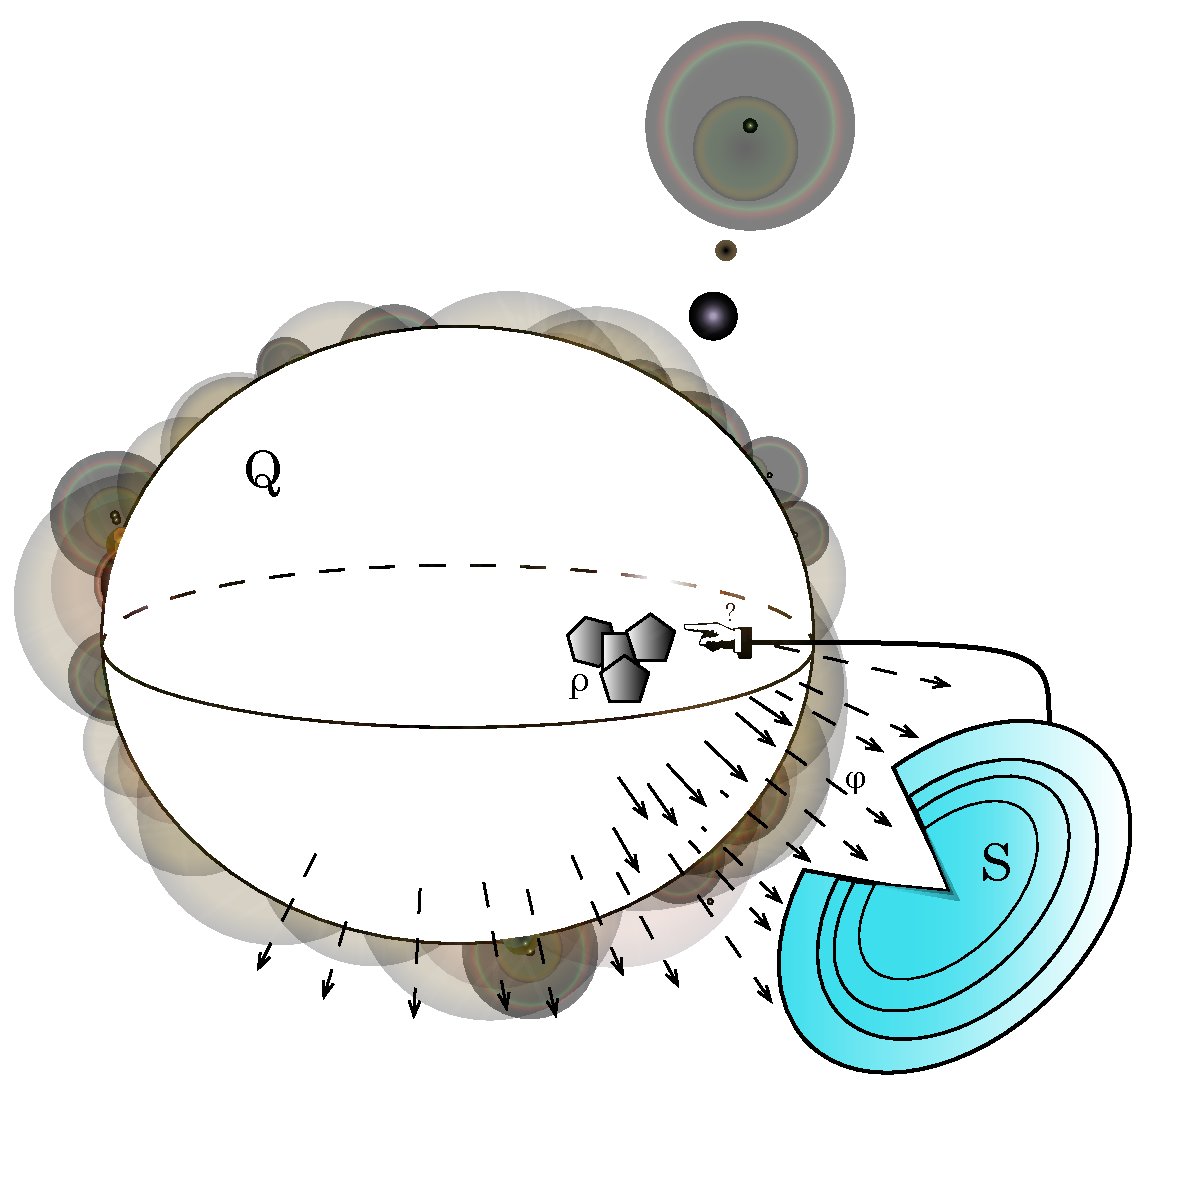
\includegraphics[width=0.8\linewidth]{tit.pdf}
}
  \caption{Геометрия задачи}
  \label{first}
  \end{figure} 

При этом возникают вопросы, насколько достоверно мы можем отыскать $\rho$
и какая поверхность $S$ лучше подойдёт для этого (например, как высоко от поверхности Земли лучше вычислять гравитационное поле).
Известно, что ОЗГ не является корректно поставленной,
поэтому во многих случаях плотность нельзя достоверно
восстановить по характеристикам порождённого ею поля.

В первой части работы сформулирована постановка обратной задачи гравиметрии, описан один из методов её решения,
детали его реализации и результаты тестов. Во второй части описывается бигармоническая задача и два алгоритма её решения, один из которых следует из ОЗГ, и происходит сравнение методов.

\section*{Обозначения}
$Q$ --- область в пространстве $\mathbb{R}^n, n\geq 2$, $S$ --- поверхность в том же пространстве,
$\bar Q = Q \bigcup \partial Q$ --- замыкание $Q$,
$Q^+= \R{n}\backslash \bar Q$ --- внешность $Q^+$,
$G(Q)$ --- подпространство гармонических в $L_2(Q)$ функций,
$N(Q)$ --- подпространство плотностей нуль-потенциалов в $L_2(Q)$,
$\nabla$ --- градиент,
$\Delta$ --- оператор Лапласа,
$E(x)= \frac{1}{2\pi}  \ln |x|, x \in Q$ --- фундаментальное решение оператора Лапласа в $\R{2}$,
$\alpha_i=\alpha_i(z)=E(z-z_i)$ --- базисный потенциал, связанный с точкой $z_i \in Q^+$,
$D^k(Q)$ --- пространство функций, $k$ раз дифференцируемых в $Q$.

\section{Определения}
Прежде чем описывать постановку ОЗГ и алгоритм её решения,
требуется определиться с несколькими достаточно простыми конструкциями,
упрощающими дальнейшее повествование.
Кроме того, необходимо пояснить, по какому принципу будут решаться поставленные задачи и что будет пониматься под устойчивостью их решения.
\subsection{Определение центра области, радиуса, подобных областей}
Пусть $Q \subset \R{n} $ -- ограниченная область с параметризуемой границей $\partial Q$, для простоты возьмём $n=2$;
сказанное значит, что $\partial Q$ можно задать радиус-вектором ${\bf r}(t)=(x(t),y(t)), t \in [t_0;t_{\max}]$.
Для достаточно универсальной и легко обслуживаемой реализации алгоритма требуется иметь задание границы области с использованием параметра $r$: ${\bf r}(t,r)=(x(t,r),y(t,r)), t \in [t_0;t_{\max}]$, где $r$ -- так называемый {\it радиус кривой} либо {\it радиус области}.
За радиус области можно взять расстояние от центра симметрии области (если такой имеется) до некоторой точки на границе, либо длину границы (периметр), либо какую-то другую характеристику;
главное -- сделать это так, чтобы при изменении параметра $r$ получалось семейство вложенных друг в друга подобных кривых. При этом при $r \rightarrow 0$ область с границей ${\bf r}(t,r)$ будет сжиматься в точку, называемую {\it центром области} либо {\it центром кривой}.

Примеры параметризации тестовых областей:
\begin{enumerate}
    \item Круг радиуса $r$ с центром в начале координат имеет границу с параметрическими функциями $x(\phi, r)=r \cos \phi, y(\phi, r)=r \sin \phi, \phi \in [0, 2\pi]$. 
     \item Внутренность квадрата со стороной $a$, у которого диагонали пересекаются в точке $(\frac{1}{2}a,\frac{1}{2}a)$, а стороны параллельны осям координат, имеет границу с параметрическими функциями:
     \[
x(t,a) =
\begin{cases}
t, & \text{если $t \in [0,a]$;} \\
a, & \text{если $t \in [a,2a]$;} \\
3a-t, & \text{если $t \in [2a,3a]$;} \\
0, & \text{если $t \in [3a,4a]$.} \\
\end{cases},
y(t,a) =
\begin{cases}
0, & \text{если $t \in [0,a]$;} \\
t-a, & \text{если $t \in [a,2a]$;} \\
a, & \text{если $t \in [2a,3a]$;} \\
4a-t, & \text{если $t \in [3a,4a]$.} \\
\end{cases}
\]
Такой квадрат при $a=4$ изображён на Рис.\ref{kvci}.
\begin{figure}[h!]
    \noindent\centering{
    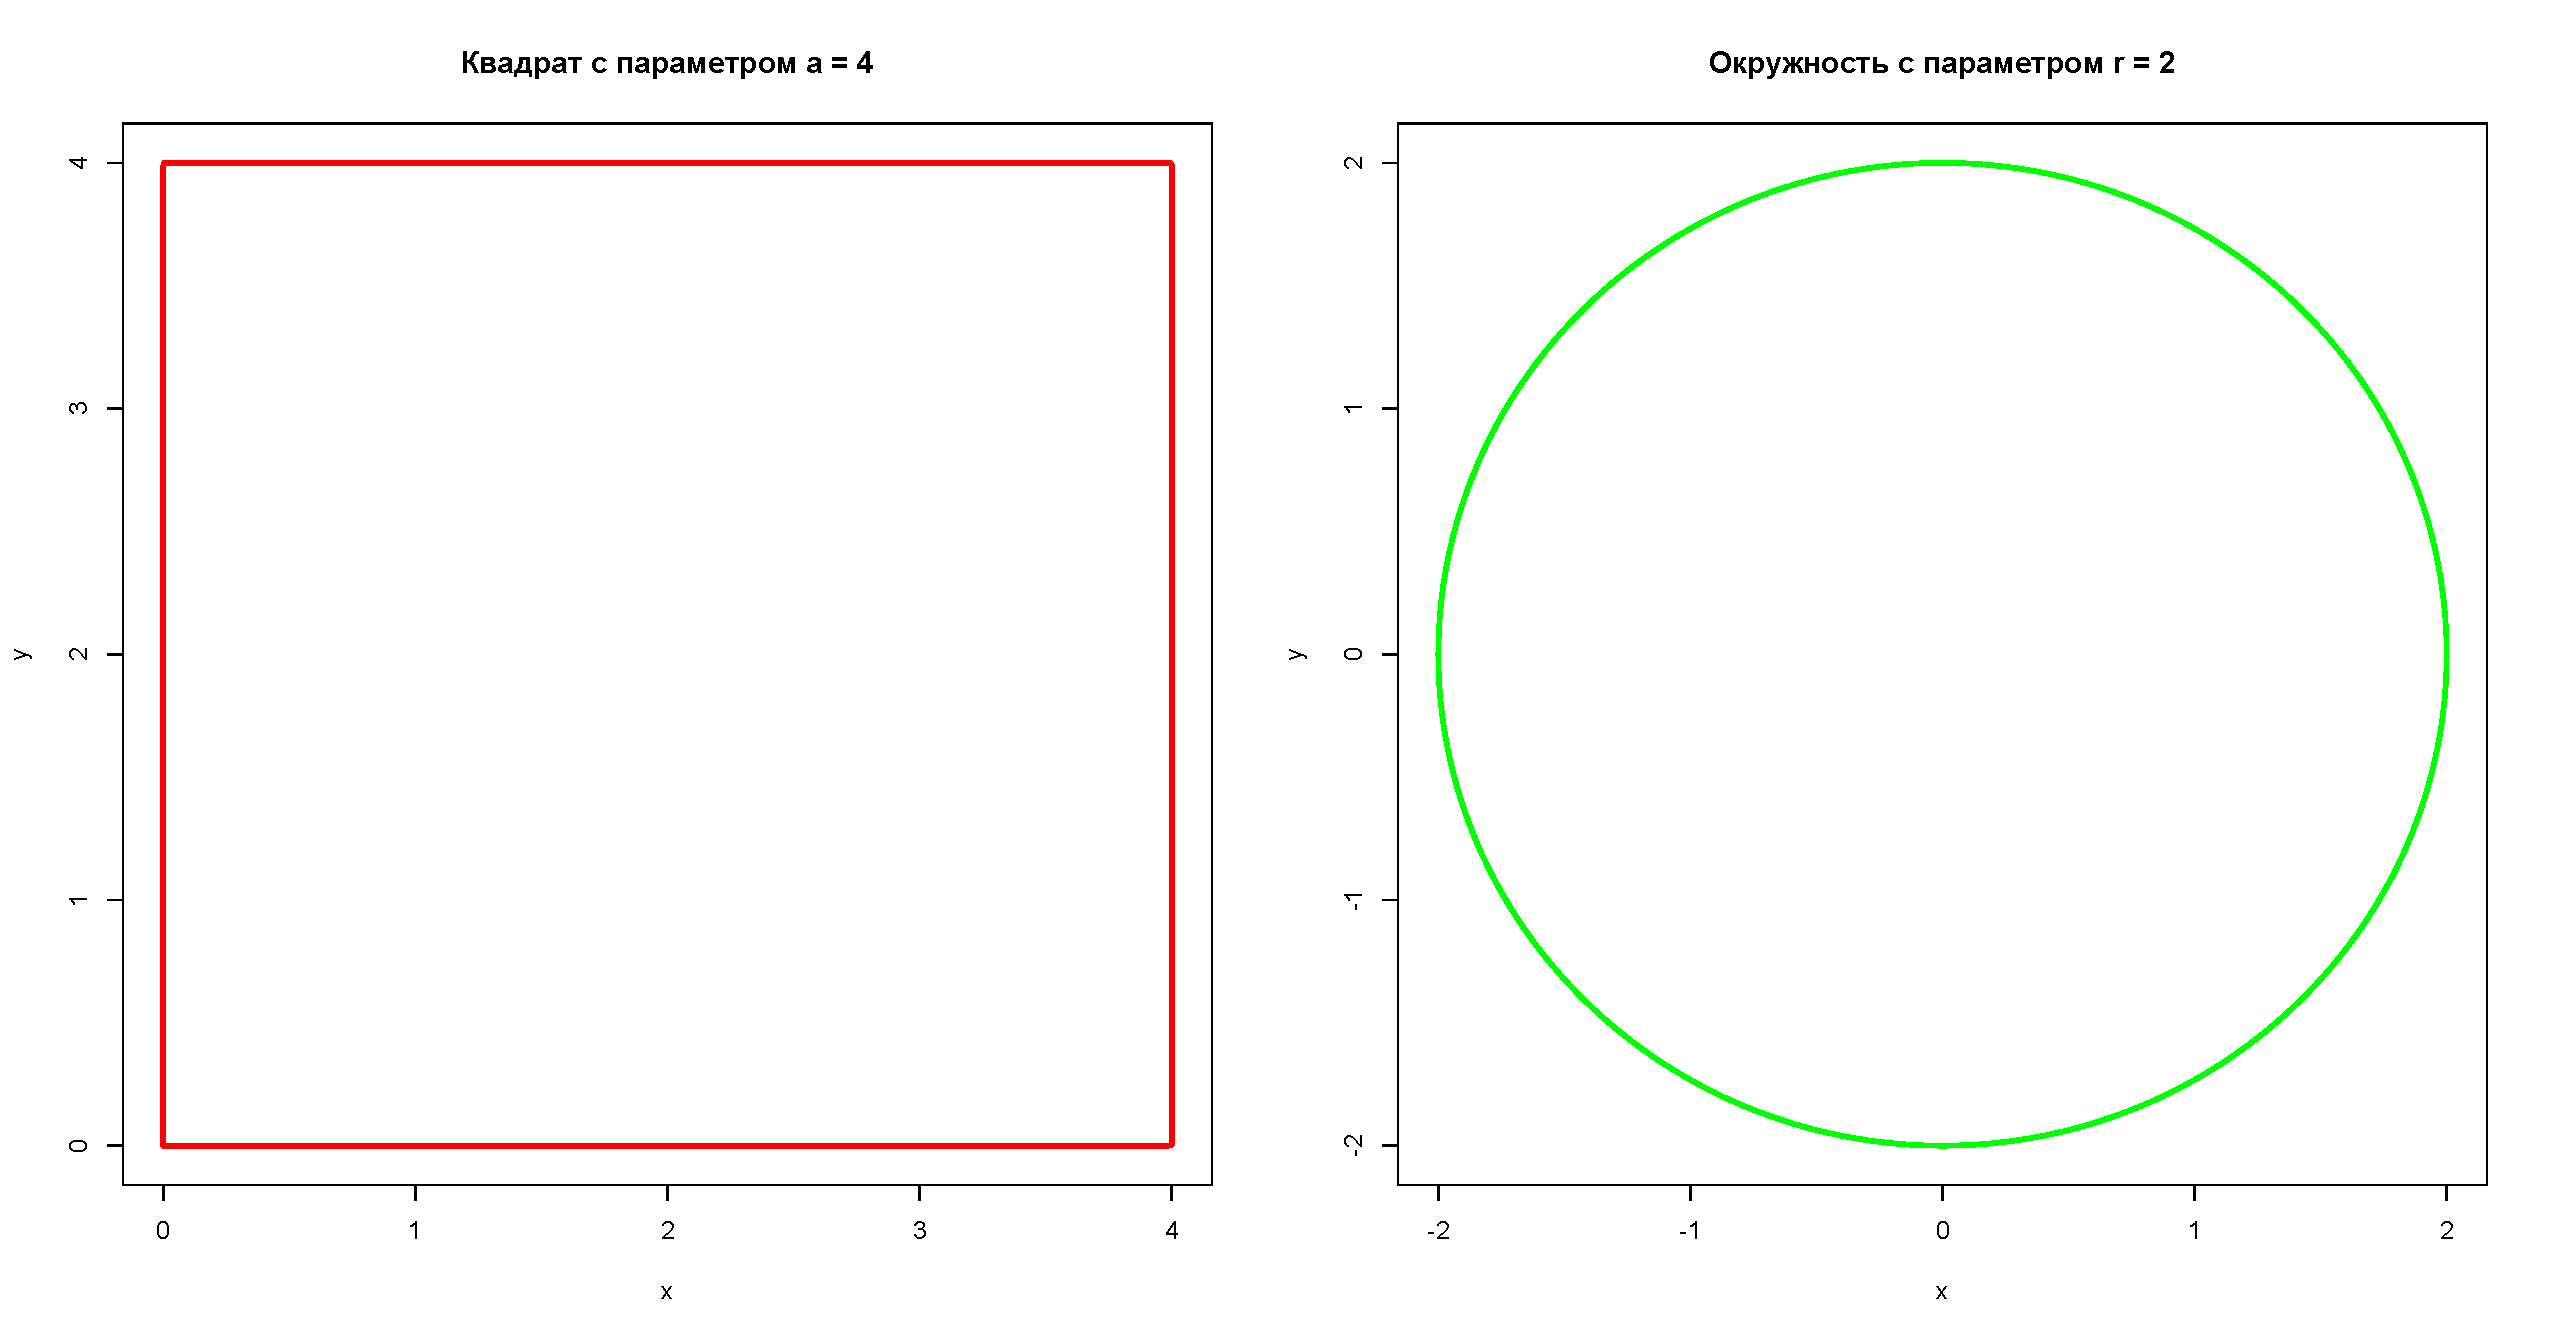
\includegraphics[width=\linewidth]{01.pdf}
  }
    \caption{Квадрат при $a=4$ и окружность при $r=2$}
    \label{kvci}
    \end{figure} 

    \item Аналогично равносторонний треугольник со стороной $a$, расположенный в первом квадранте, имеющий сторону, параллельную $oX$, и вершину в начале координат, имеет границу:
    \[
        x(t,a) =
        \begin{cases}
        t, & \text{если $t \in [0,a]$;} \\
        3a-2t, & \text{если $t \in [a,1\frac{1}{2}a]$.} \\
        \end{cases},
        y(t,a) =
        \begin{cases}
        t \sqrt{3}, & \text{если $t \in [0,\frac{1}{2}a]$;} \\
        -t \sqrt{3}+a\sqrt{3}, & \text{если $t \in [\frac{1}{2}a,a]$;} \\
        0, & \text{если $t \in [a,1\frac{1}{2}a]$.} \\
        \end{cases}
        \]
        Такой треугольник при $a=2$ изображён на Рис. \ref{tros}.

    \item Область, чья граница есть $S_1 \bigcup S_2 \bigcup S_3$, где $S_1=\{(x,y): y=0, x \in [0, a]\},S_2=\{(x,y): y=\sqrt{a^2-x^2}, x \in [\frac{1}{2}a, a]\},S_3=\{(x,y): y=\sqrt{a^2-(x-a)^2}, x \in [0,\frac{1}{2} a]\}$, может определяться через функции:       
    \[
        x(t,a) =
        \begin{cases}
        t, & \text{если $t \in [0,a]$;} \\
        2a-t, & \text{если $t \in [a,2a]$.} \\
        \end{cases},
        y(t,a) =
        \begin{cases}
        \sqrt{a^2-(t-a)^2}, & \text{если $t \in [0,\frac{1}{2}a]$;} \\
        \sqrt{a^2-t^2}, & \text{если $t \in [\frac{1}{2}a,a]$;} \\
        0, & \text{если $t \in [a,2a]$.} \\
        \end{cases}
        \]
        Такую область будем называть <<острием>>. <<Острие>> при $a=2$ изображёно на Рис. \ref{tros}.
        
        \begin{figure}[h!]
          \noindent\centering{
          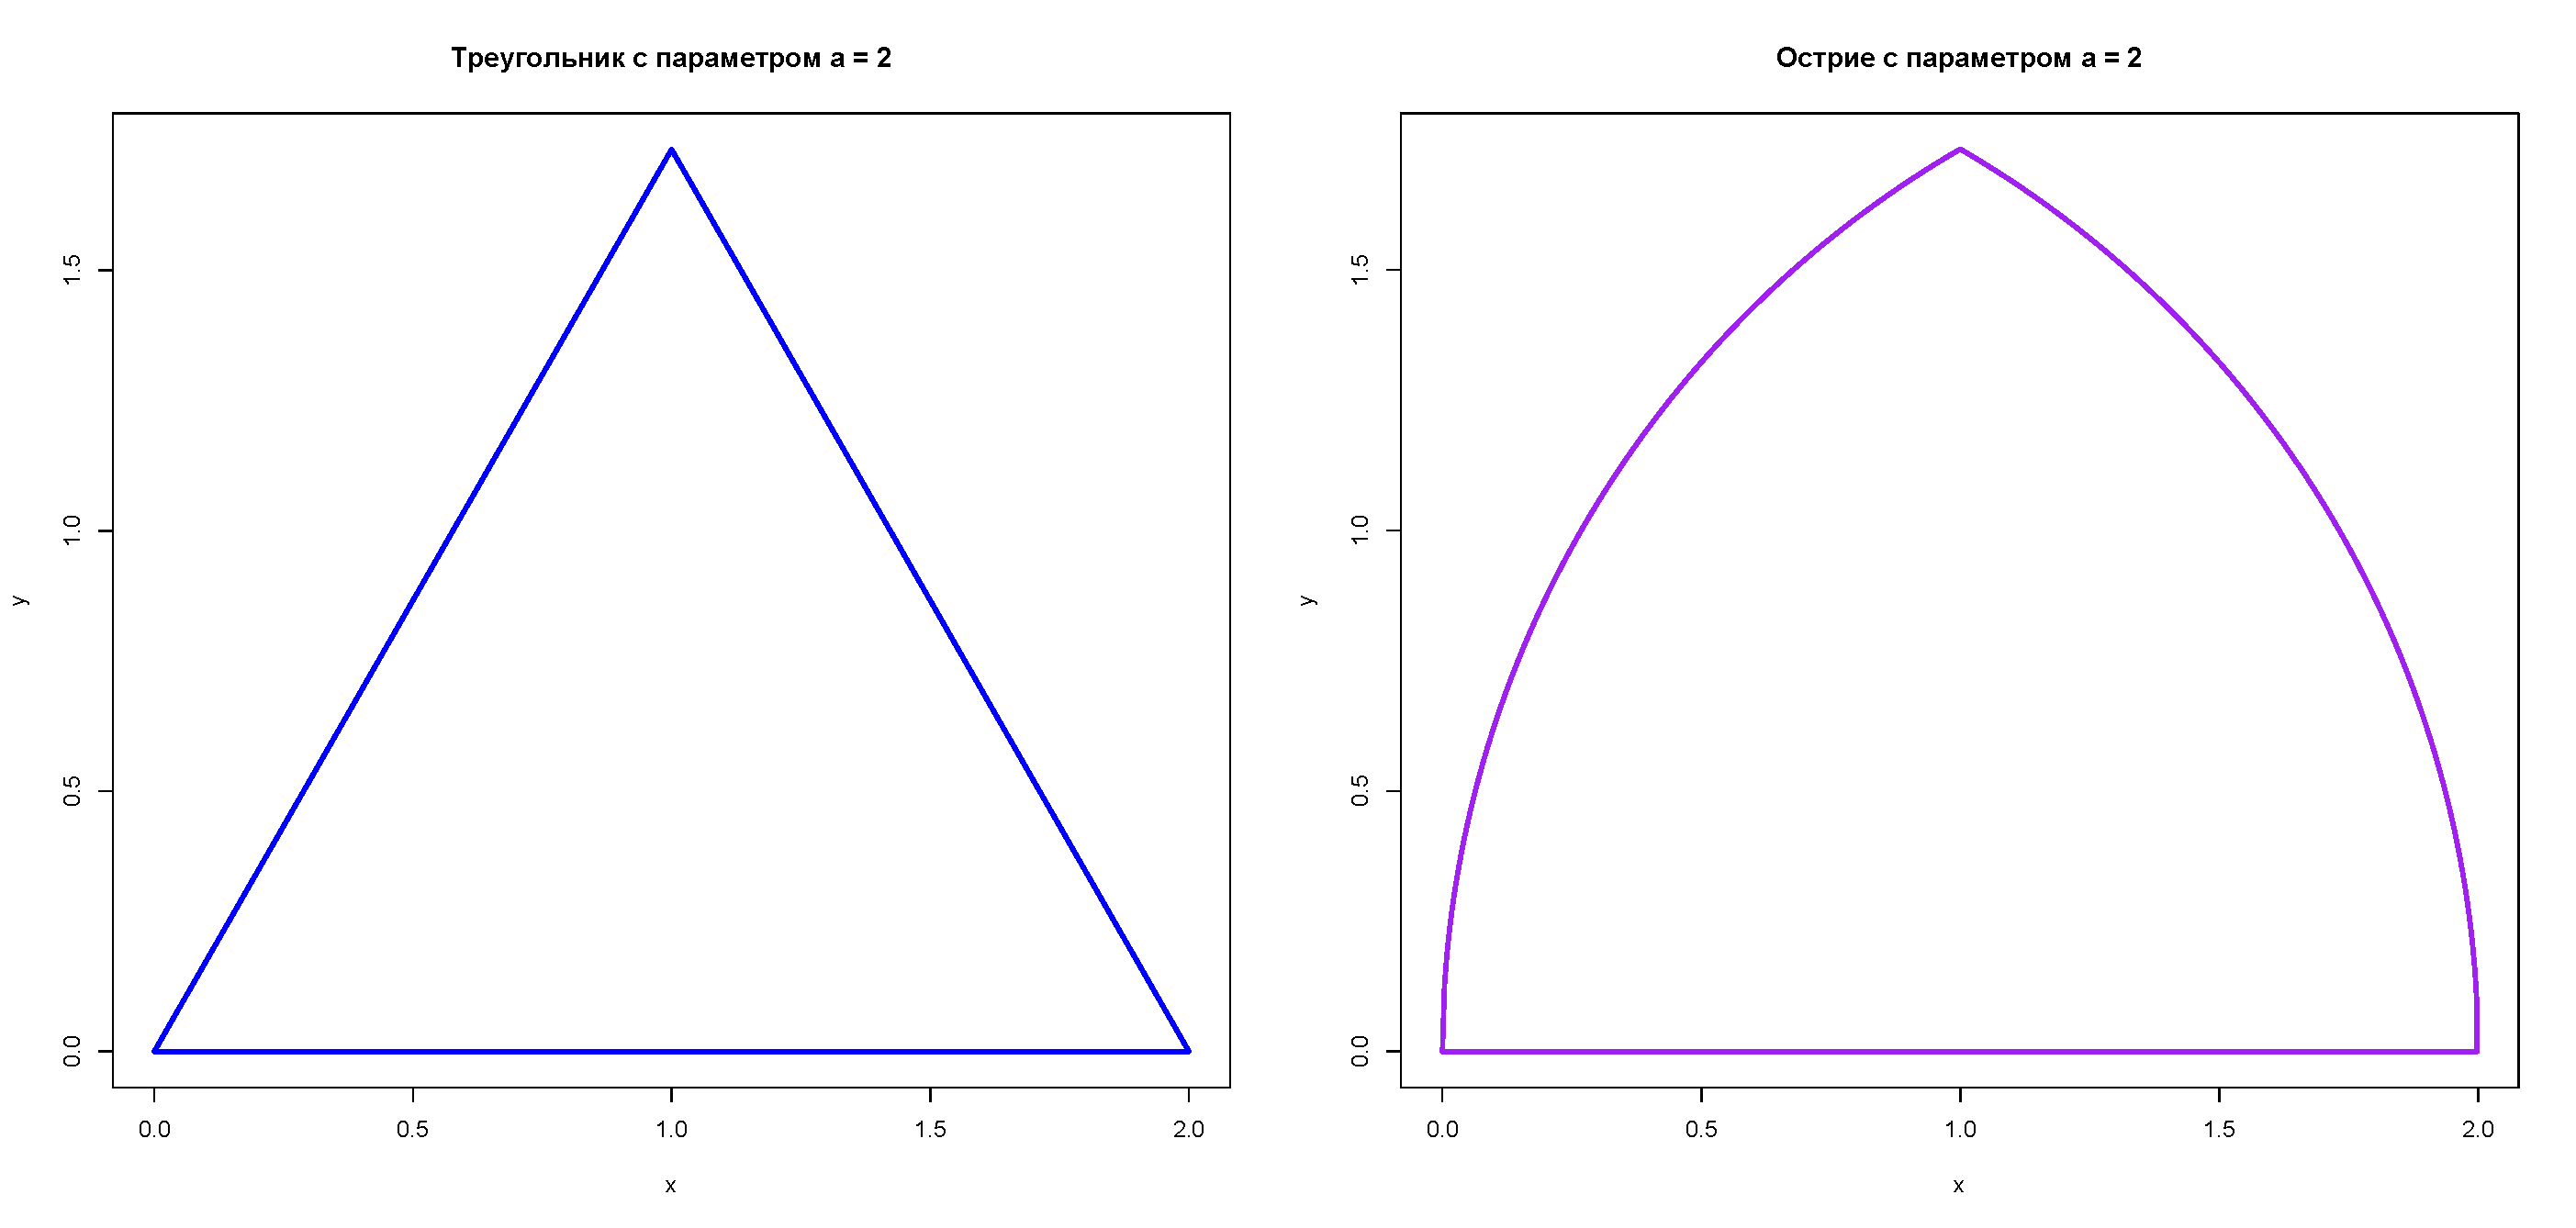
\includegraphics[width=\linewidth]{02.pdf}
        }
          \caption{Треугольник и <<острие>> при $a=2$}
          \label{tros}
          \end{figure}  
\end{enumerate}

Точно таким же образом особенно удобно задавать области, границы которых суть кусочно-гладкие кривые вида $S_i=\{(x,y): y=f_i(x), x \in [x_{i_0};x_{i_{\max}}]\}, i=1,2,\dots, n$, причём на каждом куске не имеет значения, задаётся ли кривая в декартовой системе координат или в полярной.

{\bf Замечания}:
\begin{enumerate}
  \item В указанных примерах используется простейшая параметризация, но её недостаток в том, что в некоторых примерах при изменении радиуса $r$ кривой меняется и расположение её центра, из-за чего при разных параметрах $r_1,r_2$ кривые ${\bf r}(t,r_1),{\bf r}(t,r_2)$ имеют общие точки, что не подходит для алгоритма.
Проблема исправляется фиксацией центра в некоторой точке и заданием кривых относительно этого центра. Например, квадрат с центром в $(x_0;y_0)$ и длиной стороны $a$ имеет параметризацию:
\[
x(t,a) =
\begin{cases}
x_0-\frac{1}{2}a+t, & \text{если $t \in [0,a]$;} \\
x_0+\frac{1}{2}a, & \text{если $t \in [a,2a]$;} \\
x_0+\frac{1}{2}a-(t-2a), & \text{если $t \in [2a,3a]$;} \\
x_0-\frac{1}{2}a, & \text{если $t \in [3a,4a]$.} \\
\end{cases},
y(t,a) =
\begin{cases}
y_0-\frac{1}{2}a, & \text{если $t \in [0,a]$;} \\
y_0-\frac{1}{2}a+(t-a), & \text{если $t \in [a,2a]$;} \\
y_0+\frac{1}{2}a, & \text{если $t \in [2a,3a]$;} \\
y_0+\frac{1}{2}a-(t-3a), & \text{если $t \in [3a,4a]$.} \\
\end{cases}.
\]
Теперь, меняя значение параметра $a$, мы получаем вложенные друг в друга квадраты с общим центром (Рис. \ref{rects}).
\begin{figure}[h!]
  \noindent\centering{
  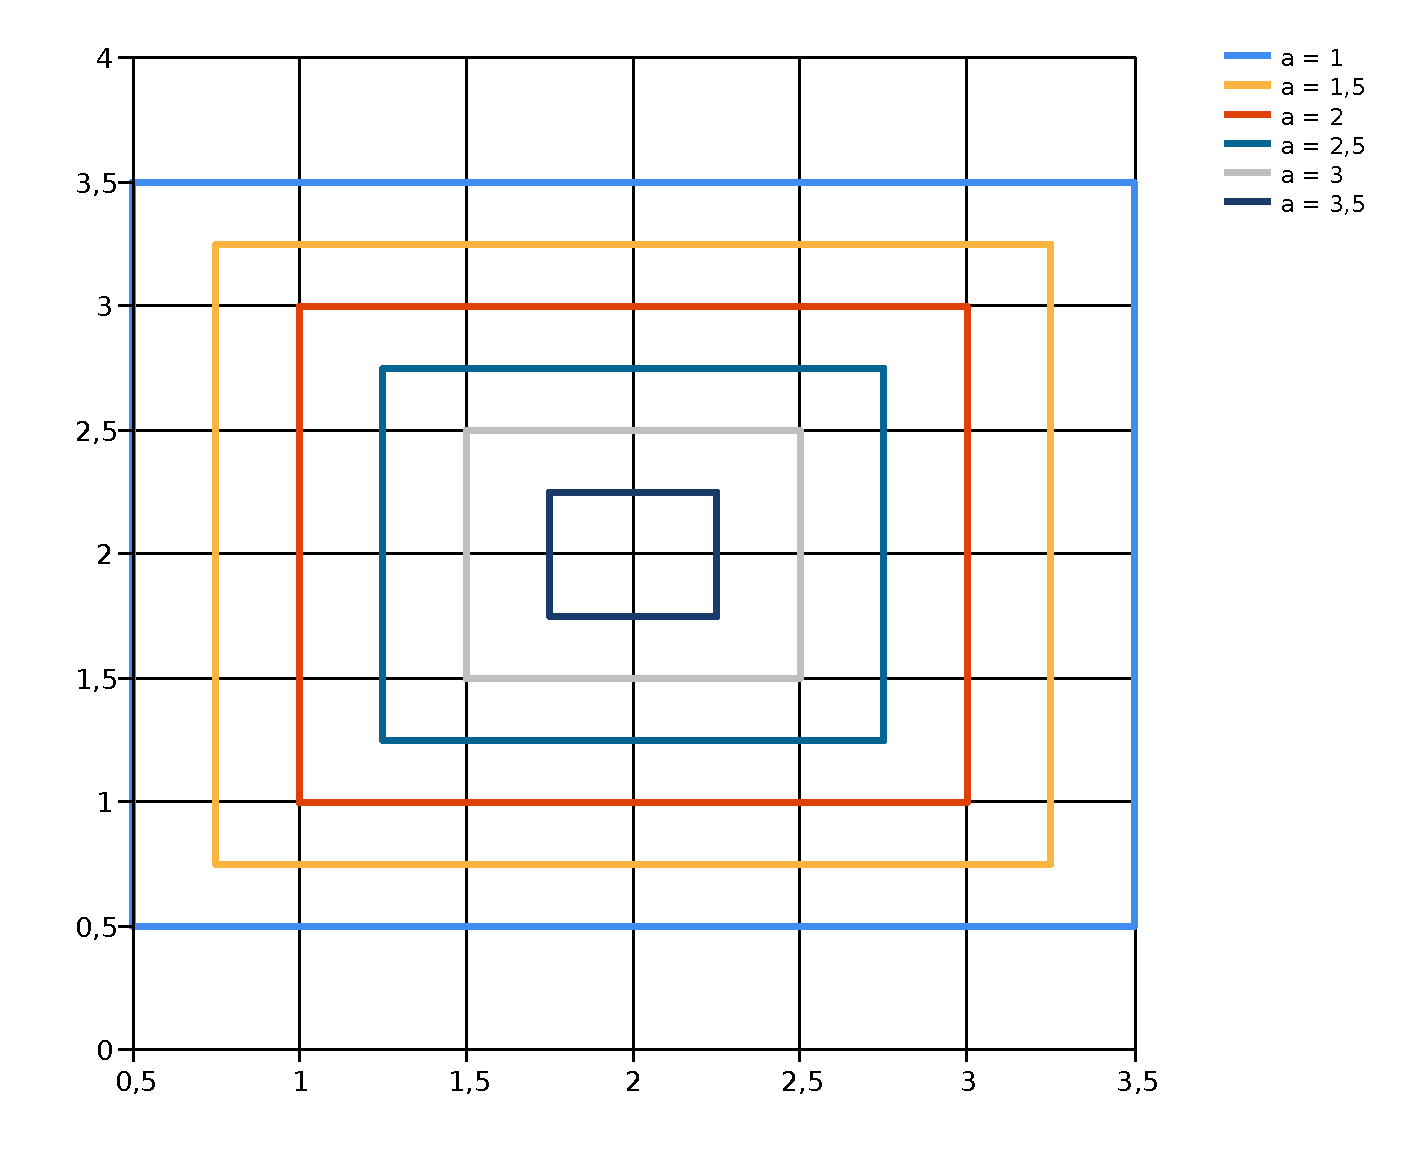
\includegraphics[width=0.7\linewidth]{rect.pdf}
}
  \caption{Вложенные квадраты с центром $(2;2)$}
  \label{rects}
  \end{figure}
  
  \item Если кривая уже задана параметрическими функциями $x=x(t),y=y(t)$,
  чаще всего (кроме случаев, когда она проходит через некоторый центр,
  относительно которого задана\footnote{К примеру, для окружности естественным будет её геометрический центр, но если взять замкнутую полуокружность (концы соединены друг с другом отрезком), то естественным будет задать эту полуокружность относительно центра окружности, но в этом случае она будет проходить через центр, поэтому такая параметризация не может использоваться, т. к. с уменьшением радиуса происходит сжатие не во внутрь фигуры. В нетривиальных случаях следует в качестве центра области использовать центр масс области.}) подобные вложенные кривые можно получить домножением $x,y$ на радиус $r$.
  В этом случае даже не очевидно, что именно является "центром"\ кривой, но этот центр легко сдвигать прибавлением к $x,y$ координат вектора переноса.
  На рисунках \ref{rr1}-\ref{rr2} это правило используется для базовой кривой, заданной формулами
\[
\begin{cases}
  x(t)=(R-r)\cos\left(\frac{r}{R}t\right)+h \cos \left(t-\frac{r}{R}t\right),\\
  y(t)=(R-r)\sin\left(\frac{r}{R}t\right)-h \sin \left(t-\frac{r}{R}t\right),\\
  r=\dfrac{1}{3}, h=\dfrac{1}{4}
\end{cases}.  
\]

  \begin{figure}[h]
    \begin{center}
    \begin{minipage}[h]{0.49\linewidth}
    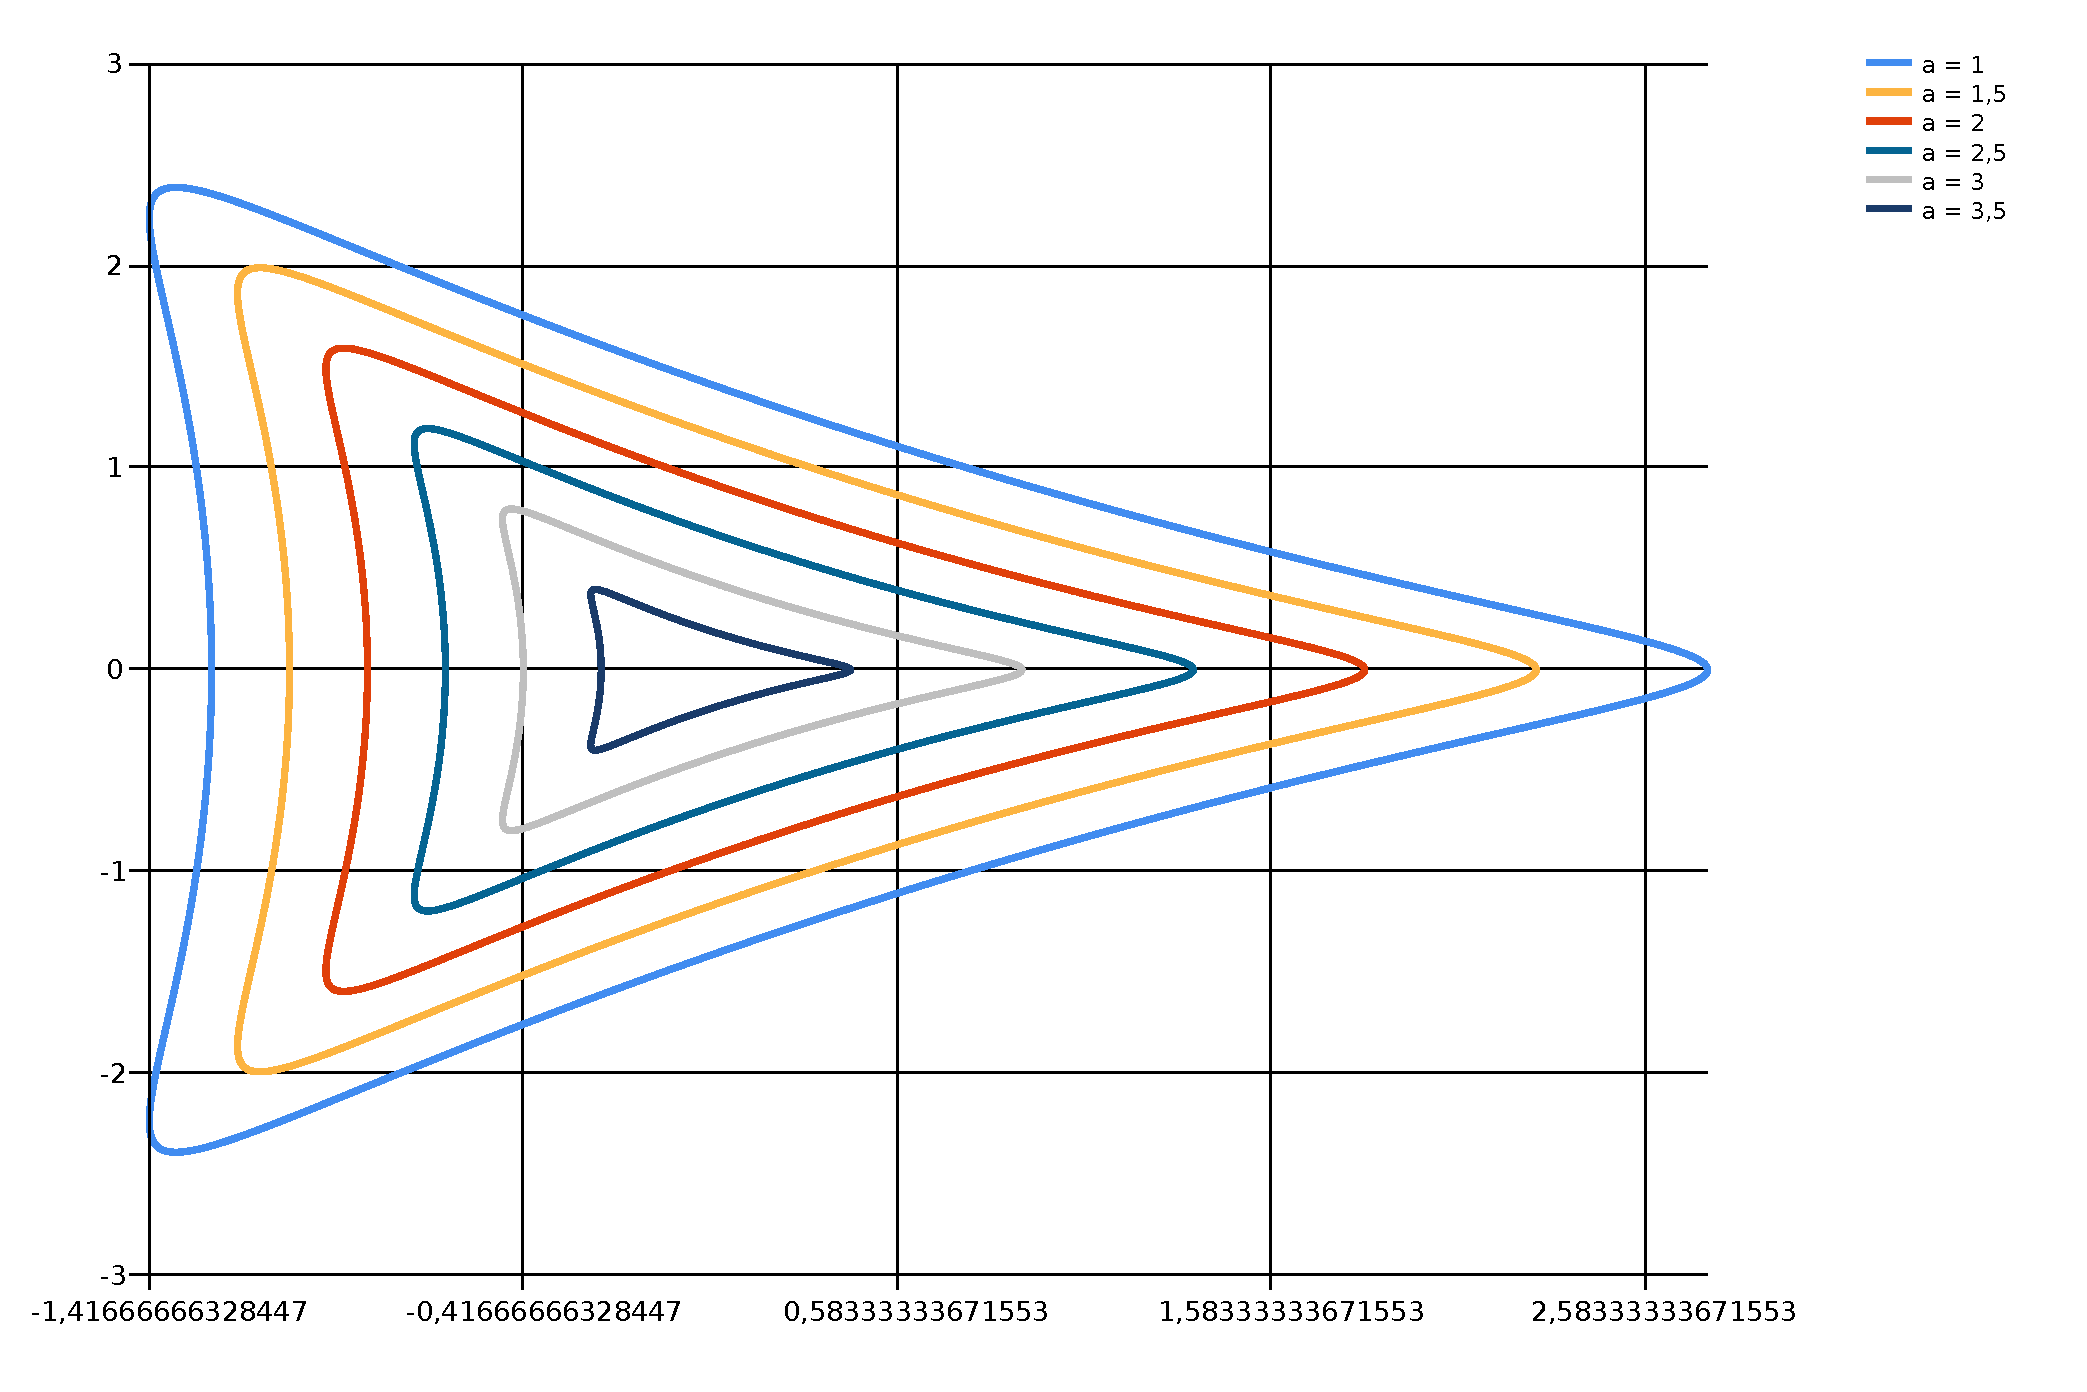
\includegraphics[width=1\linewidth]{r1.pdf}
    \caption{$R=1$} %% подпись к рисунку
    \label{rr1} %% метка рисунка для ссылки на него
    \end{minipage}
    \hfill 
    \begin{minipage}[h]{0.49\linewidth}
    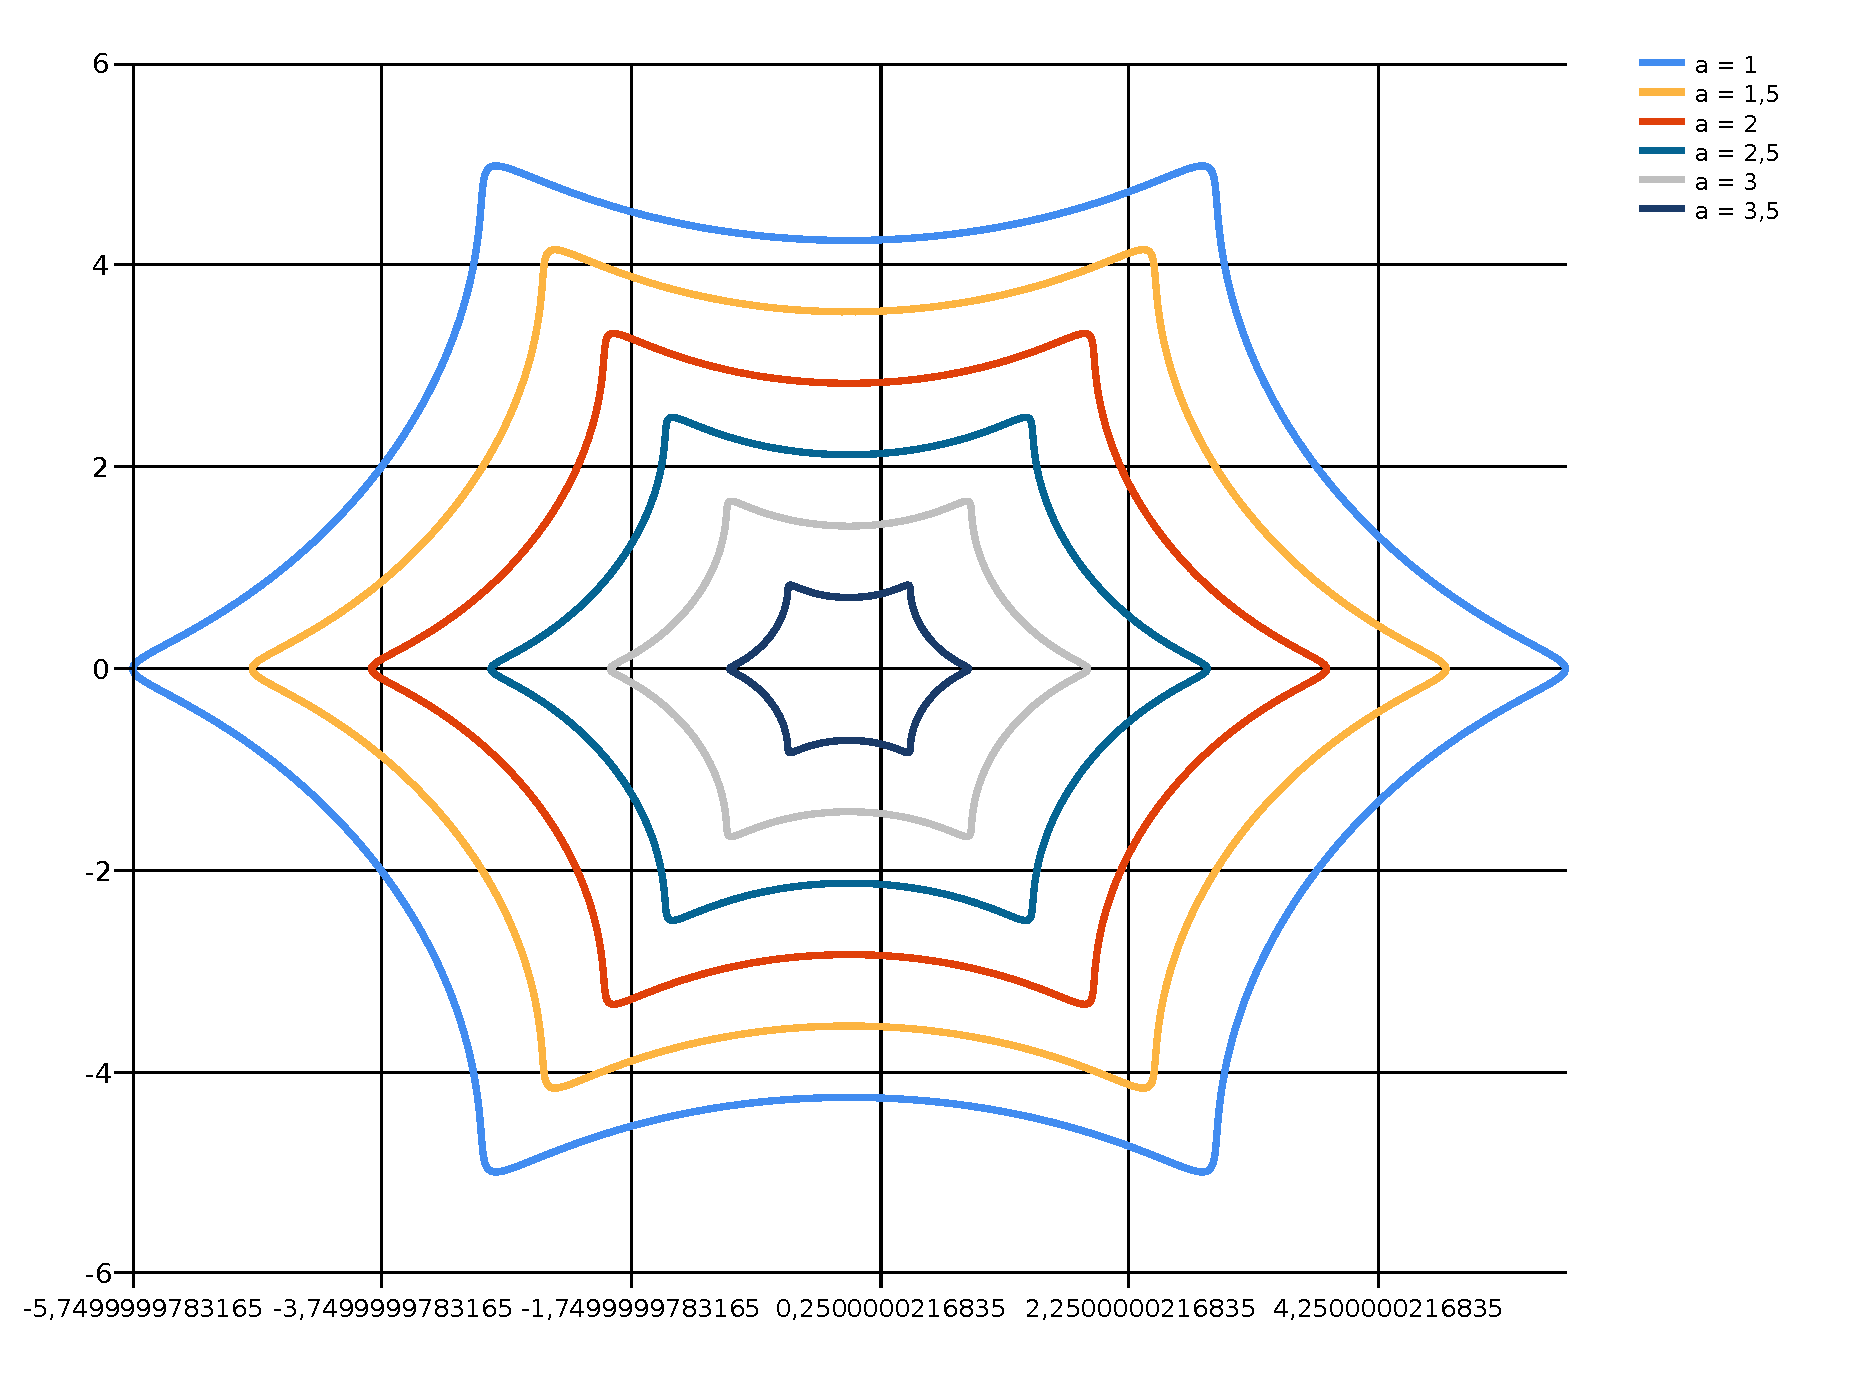
\includegraphics[width=1\linewidth]{r2.pdf}
    \caption{$R=2$}
    \label{rr2}
    \end{minipage}
    \end{center}
    \end{figure}
\end{enumerate}

\FloatBarrier 
\subsection{Определение целевой и побочной задачи, неустойчивости решения на примере полиномиальной интерполяции}
Пусть требуется решить некоторую задачу, например, приблизить сложную функцию $f: \mathbb{R} \rightarrow \mathbb{R}$
на некотором отрезке $[x_{\min};x_{\max}]$ более простой функцией $g=g(x,{\bf c})$, зависящей от параметров (вектора ${\bf c}$), которые и следует подобрать.
Это значит, что нужно найти некоторый вектор ${\bf \tilde{c} }$, при котором
\begin{equation*}
  ||f-g({\bf \tilde{c}})|| < \varepsilon,
\end{equation*}
где $\varepsilon$ --- некоторая приемлемая погрешность, а $||\cdot||$ --- равномерная либо среднеквадратичная норма.
Такую задачу будем называть {\it целевой, основной}.

Допустим, нельзя решить целевую задачу прямым образом (нельзя приближать $f$ сразу по всем точкам отрезка), но можно приближать $f$ на некотором наборе точек $x_i \in [x_{\min};x_{\max}], i=1,\dots,n$.
Эту задачу будем называть {\it побочной}. Таким образом,
мы будем искать решение побочной задачи (в данном случае --- задачи интерполяции),
рассчитывая, что решение побочной задачи будет и решением целевой задачи (задачи аппроксимации).

Такой подход не всегда может дать эффективное решение. Например, задача интерполяции полиномами по определению решается точно,
но для неё существует феномен Рунге (появление возрастающих осцилляций при интерполяции полиномами высокой степени, Рис. \ref{l1}-\ref{l2}),
из-за которого интерполирующая функция не обязательно будет приближать интерполируемую функцию на всём отрезке
(более того, для примера Рунге доказано, что с ростом степени полинома погрешность устремляется к бесконечности\footnote{См. \url{https://en.wikipedia.org/wiki/Runge\%27s_phenomenon} }).

\begin{figure}[!h]
  \begin{center}
  \begin{minipage}[h]{0.49\linewidth}
  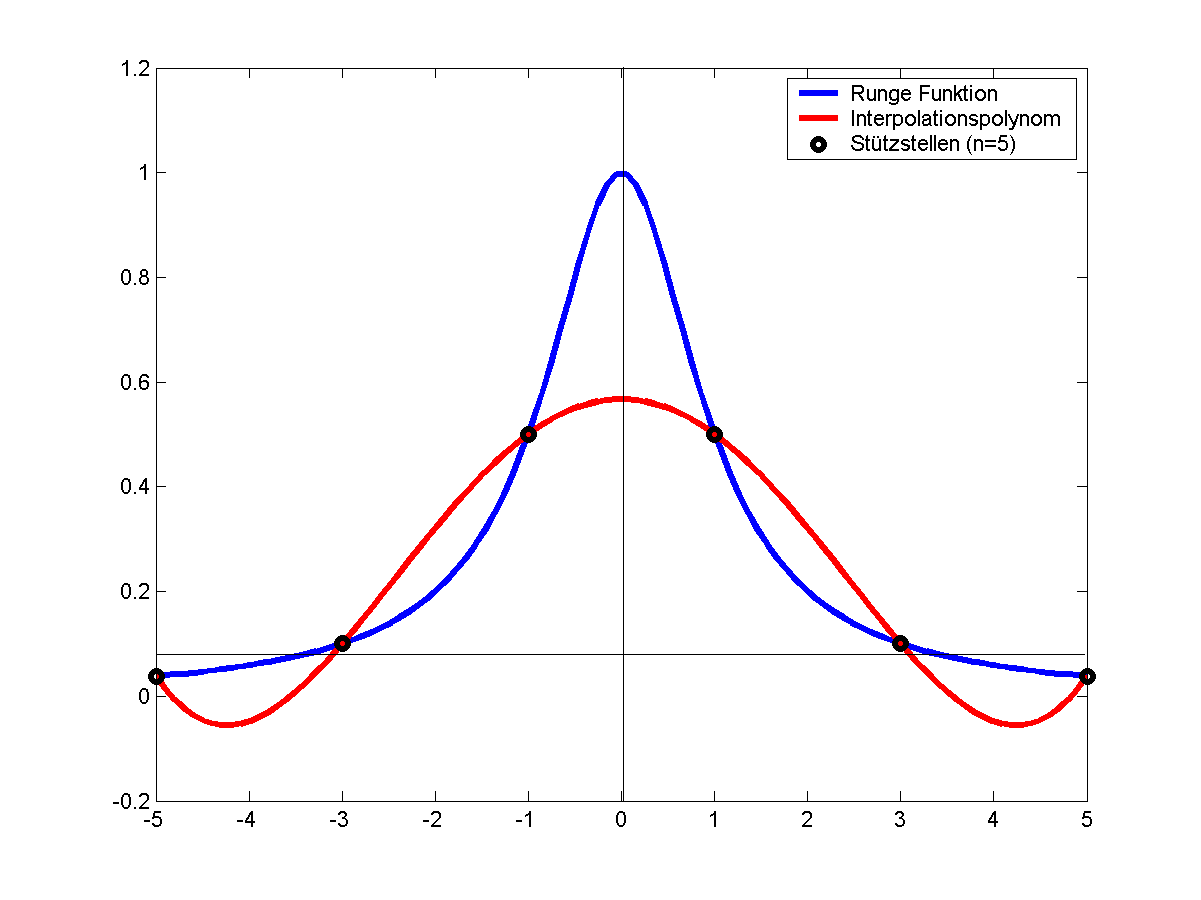
\includegraphics[width=1\linewidth]{f1.png}
  \caption{Интерполяция функции $\dfrac{1}{1+x^2}$ полиномом степени 5} %% подпись к рисунку
  \label{l1} %% метка рисунка для ссылки на него
  \end{minipage}
  \hfill 
  \begin{minipage}[h]{0.49\linewidth}
  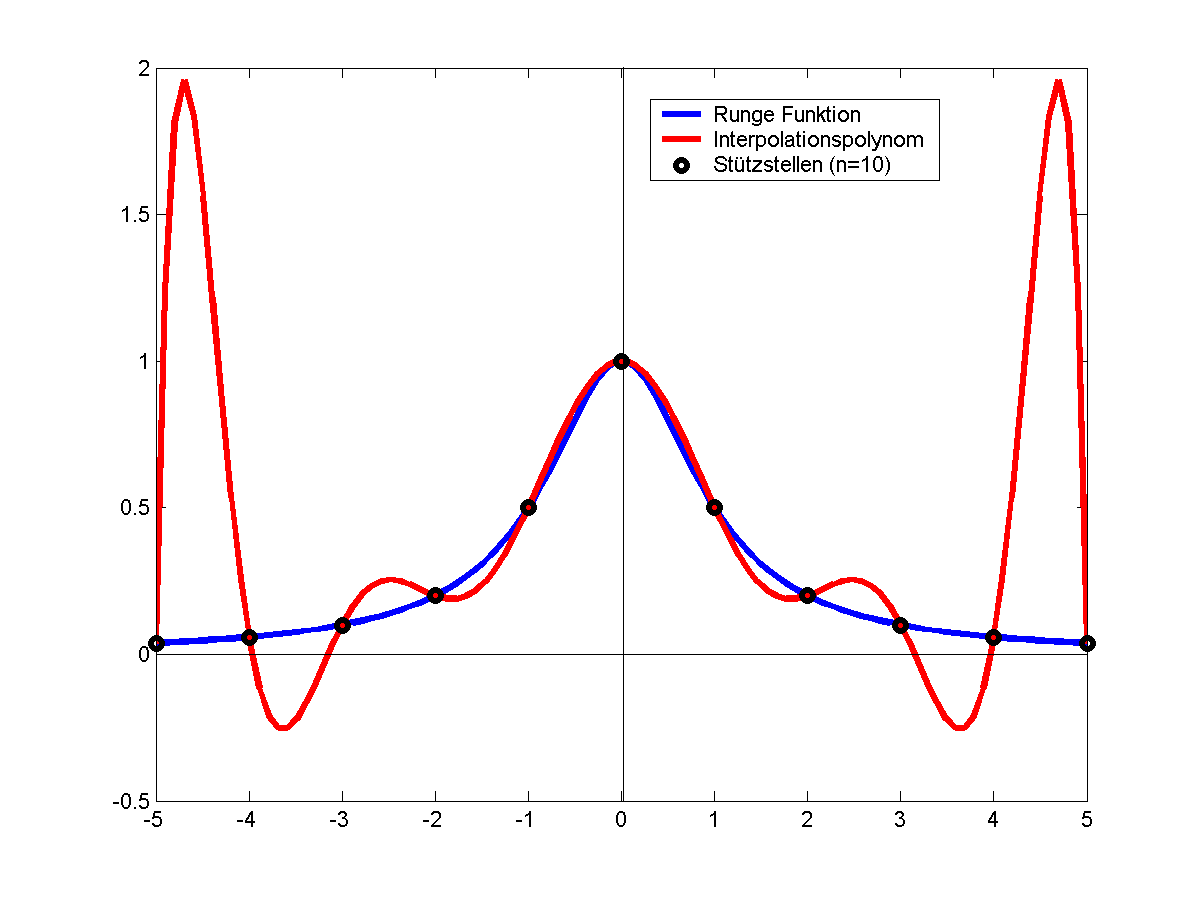
\includegraphics[width=1\linewidth]{f2.png}
  \caption{Интерполяция функции $\dfrac{1}{1+x^2}$ полиномом степени 10, появление осцилляций}
  \label{l2}
  \end{minipage}
  \end{center}
  \end{figure}

График зависимости погрешности аппроксимации от числа наблюдений (точек для интерполяции) будет иметь примерно такой же вид, как на Рис.\ref{runge1}-\ref{runge2}, то есть
сначала погрешность целевой задачи будет уменьшаться, затем поднимется до пика, затем опять уменьшится и т. д.

\begin{figure}[!h]
  \noindent\centering{
  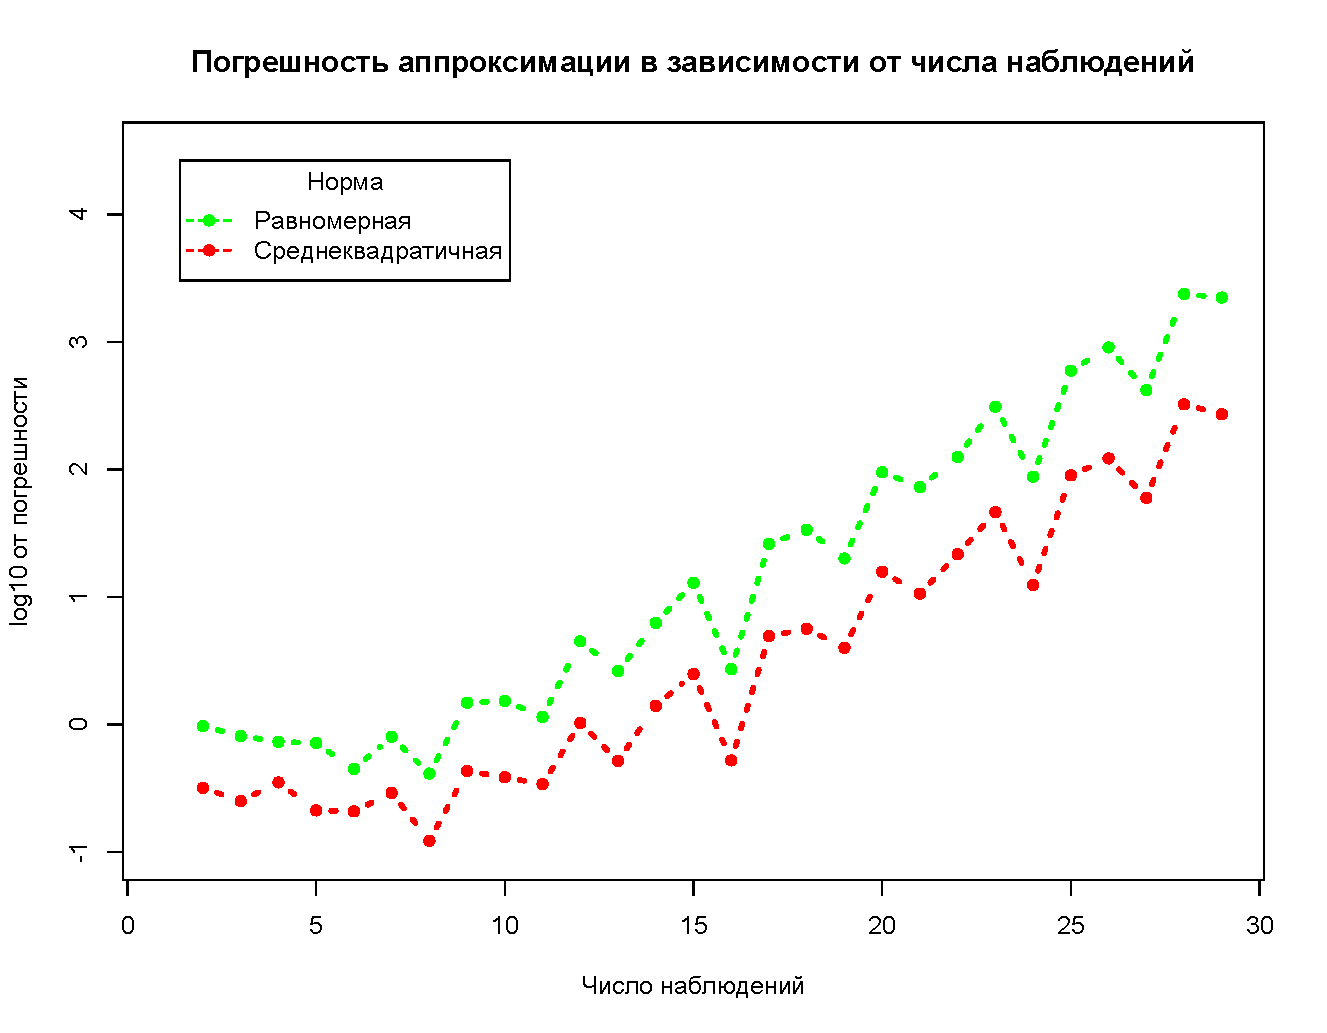
\includegraphics[width=0.6\linewidth]{Runge1.pdf}
  }
  \caption{Неустойчивость интерполяции для $f(x)=\dfrac{1}{1+x^2}$ на $[-9,5]$}
  \label{runge1}
\end{figure}
\begin{figure}[!h]
  \noindent\centering{
  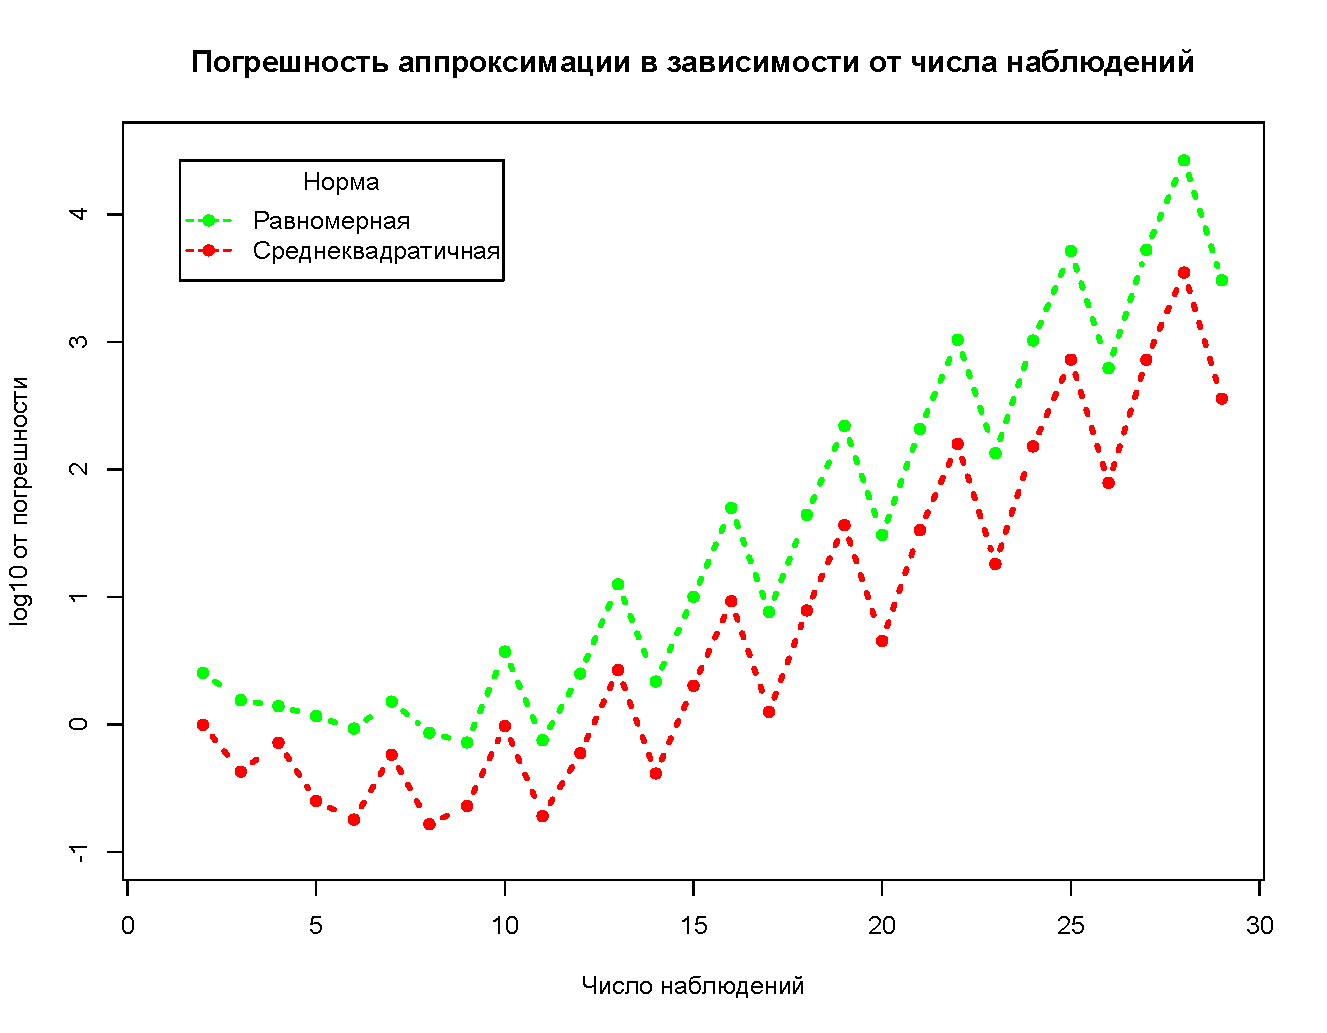
\includegraphics[width=0.6\linewidth]{Runge2.pdf}
  }
  \caption{Неустойчивость интерполяции для $f(x)=\sqrt{|x|}$ на $[-5,10]$}
  \label{runge2}
\end{figure}

Такое поведение погрешности при расширении числа наблюдений / аппроксимирующего подпространства будем называть {\it нестабильным, неустойчивым}; обратное поведение, т. е. невозрастание погрешности, будем называть {\itустойчивостью}.
Неустойчивость какого-то алгоритма решения практически обнуляет его значимость,
так при решении целевой задачи для любого числа $k$ наблюдений нельзя быть уверенным, что полученное решение окажется лучше, чем решение при $\frac{1}{2}k$ наблюдений, или вообще может считаться решением.    

\section{Обратная задача гравиметрии (ОЗГ)}
\subsection{Постановка задачи}
Пусть $Q\subset \R{n}, n=2,3$ --- ограниченная область с ляпуновской границей,
$S \subset \R{n}\backslash Q$ --- достаточно гладкая поверхность (расположенная произвольно относительно $Q$), $\varphi: S \rightarrow \mathbb{R}$ --- действительная функция, заданная на $S$.
Требуется найти плотность $\rho \in L_2(Q) \bigcap G(Q)$ из выражения
\begin{equation}
    \forall x \in S: V_\rho(x)= \V{\rho}= \varphi(x).
\end{equation}

Хорошо известно, что ОЗГ не является однозначно разрешимой, но Новиков П. С. в 1938 г. доказал следующий результат, позволяющий надеяться на частичное решение:
по лемме Новикова (\cite{lezh}, стр. 56, \cite{nov}, стр. 123-126) для любой области $Q$ с ляпуновской границей пространство $L_2(Q)$ раскладывается в прямую сумму 
\begin{equation}
    L_2(Q)= G(Q) \oplus N(Q),
\end{equation}
где $G(Q)$ --- пространство гармонических на $Q$ функций, $N(Q)$ --- пространство всех функций $\psi$, таких что
\begin{equation}
    \V{\psi}=0, \forall x\in Q^+,
\end{equation}
называемое пространством плотностей нуль-потенциалов в $L_2(Q)$.

Описанный результат значит, что $\forall \beta \in L_2(Q) \ \beta = \beta_1 + \beta_2, \beta_1 \in G(Q), \beta_2 \in N(Q)$, $\V{\beta}=\V{\beta_1}$ независимо от $\beta_2$, то есть для любой плотности $\rho$ возможно найти только её гармоническую компоненту.   


\subsection{Алгоритм приближённого решения}

Далее описывается один из алгоритмов решения ОЗГ, а также приводятся некоторые детали реализации.

\subsubsection{Описание алгоритма решения ОЗГ}
Расположим в открытом множестве $Q^+= \R{n}\backslash \bar Q$ точки $z_1,z_2,\dots,z_N$ (базисные точки). От положения этих точек будет зависеть точность решения, однако пока неизвестно, какое именно положение точек будет оптимальным.
Известно, что во многих случаях существуют наборы точек, дающие наилучшее решение задачи вплоть до машинного нуля, как есть и крайне неоптимальные наборы точек, которые не будут давать точного решения даже в тривиальном случае.
Во всяком случае, точки требуется располагать по какому-то правилу, чтобы результаты экспериментов можно было сравнивать.
Пока будем располагать точки равномерно возле подобной $S$ поверхности большего радиуса, при этом сами точки должны располагаться с небольшими случайными отклонениями в ту или другую сторону по нормали от $S$ (Рис. \ref{sample}).

\begin{figure}[!h]
    \noindent\centering{
    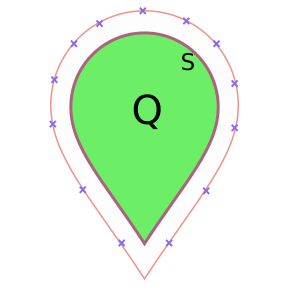
\includegraphics[width=120mm]{il1}
    }
    \caption{Образец расстановки базисных точек в $\R{2}$}
    \label{sample}
\end{figure}


Расставив точки, будем искать приближённое решение ОЗГ $\tilde \rho_N$ в виде
\begin{equation}
    \tilde \rho_N=\sum_{i=1}^N c_i \alpha_i,
\end{equation}
где $\alpha_i=\alpha_i(z)=E(z-z_i),c_i \in \mathbb{R}$ определяются из решения задачи минимизации функционала
\begin{equation}
    F({\bf c})=F(c_1,\dots,c_N)=\Bigr|\Bigr|V_{\sum_{i=1}^N c_i \alpha_i} -\varphi\Bigr|\Bigr|_{L_2(S)} \rightarrow \min, \varphi =V_{\rho} \equiv \V{\rho}. 
\end{equation}

Нетрудно показать, что $F$ --- квадратичный функционал, а задача его минимизации эквивалентна решению системы линейных алгебраических уравнений
\begin{equation}
    \begin{pmatrix}
        (\omega_1, \omega_1) & (\omega_1, \omega_2) & \cdots & (\omega_1, \omega_N)\\
        (\omega_2, \omega_1) & (\omega_2, \omega_2) & \cdots & (\omega_2, \omega_N)\\
        \hdotsfor{4}\\
        (\omega_N, \omega_1) & (\omega_N, \omega_2) & \cdots & (\omega_N, \omega_N)\\
    \end{pmatrix}
    \begin{pmatrix}
        c_1\\
        c_2\\
        \cdots\\
        c_N\\
    \end{pmatrix}
    =
    \begin{pmatrix}
        (\omega_1,\varphi)\\
        (\omega_2,\varphi)\\
        \cdots\\
        (\omega_N,\varphi)\\
    \end{pmatrix},
    \label{gram}
\end{equation}
где 
\begin{equation}
    \omega_i(x)=\V{\alpha_i}
\end{equation}
и скобки $(\cdot,\cdot)$ обозначают скалярное произведение:
\begin{equation}
    (f,g)=(f,g)_{L_2(S)}=\int_S f(x)g(x) ds.
\end{equation}

Заметим, что мы свели решение ОЗГ к решению задачи аппроксимации функции $\varphi$ системой функций $\omega_i$. 

\subsubsection{Детали реализации}
{\itКратное интегрирование}. Для интегрируемой функции $f$ и области $Q$ на прямоугольной области $D \supseteq Q$ определим функцию
\begin{equation*}
  g(x)=
  \begin{cases}
    f(x), & x \in Q\\
    0, & x \not \in Q
  \end{cases}.
\end{equation*}
В программной реализации интеграл от функции $f$ считается как интеграл от функции $g$ методами библиотеки Math.NET Numerics (\url{https://numerics.mathdotnet.com})
по квадратурам Гаусса-Лежандра при числе узлов $n=128$.

До этого автором использовались лично написанные методы интегрирования, которые  не удовлетворяли либо в точности, либо по производительности, поэтому было решено использовать сторонние методы.

{\itУстойчивое решение СЛАУ, связанной с задачей аппроксимации}. Известно, что матрица системы (\ref{gram}) --- это матрица Грама, а численное решение такой системы составляет отдельную задачу, поскольку классические методы решения и их простые комбинации дают неустойчивое решение.
Наибольший вклад в неустойчивость аппроксимации вносят три причины:

\begin{enumerate}
\item  Скалярные произведения, заполняющие СЛАУ, обычно представляются конечными суммами или интегралами; при этом это могут быть интегралы по сложным областям или поверхностям или интегралы от функций, которые сами задаются интегралами; в таком случае погрешности квадратурных формул накапливаются и приводят к тому, что исходная СЛАУ несколько отличается от истинной, что негативно сказывается на решении задачи. Даже если удаётся подобрать реализуемый способ интегрирования, часто попытки повысить точность существенно увеличивают время вычислений.

\item  Матрица Грамма для любой системы функций является плохо обусловленной по определению, причём число обусловленности быстро растёт с увеличением размерности, из-за чего даже малые отклонения в элементах системы (которые будут иметь место хотя бы по причине пункта 1) приводят к неточным решениям.

\item  Огромную роль играют погрешности округления при суммировании больших и маленьких чисел, делении и умножении; эти погрешности заметны при вычислении интегралов, решении СЛАУ и даже при замене координат (для получения системы, ортогональной на произвольном отрезке).
При плохо обусловленной матрице системы даже итерационные методы не способны из-за ошибок округления приблизиться к истинному решению ближе некоторого расстояния. Комбинация пунктов 1) и 3) приводит к тому, что даже аппроксимация по  ортогональным системам обладает неустойчивостью при достаточно большом числе функций.
\end{enumerate}

Имеется алгоритм решения таких систем, дающий устойчивое решение, который и будет использован.
Назовём его {\it ультра-гибридным} .
Он заключается в следующем. Допустим, требуется минимизировать функционал вида
\begin{equation}
  F\left({\bf c}^M\right)={\left\|\varphi -\sum^M_{m=1}{c_m}{\alpha }_m\right\|}_{{\ L}_2\left(\partial Q\right)},\ {\bf c}^M=(c_1,\dots,c_M),\ \text{функции } \varphi, \alpha_m \text{ известны},
\end{equation} 
причём его МИНИМ. должна удовлетворять условию
\begin{equation}F\left({\bf c}^{M-1}\right)\ge F\left({\bf c}^M\right)\ge F\left({\bf c}^{M+1}\right),\ M\ge 2.
\end{equation} 
Такую минимизацию можно осуществить по индукции:

Если $M=1$, решение очевидно: ${\bf c}^1=c_1=\left({\alpha }_1,\varphi \right)/\left({\alpha }_1,{\alpha }_1\right)$. В противном случае требуется искать решения для ${\bf c}^2$, ${\bf c}^3$,{\dots}, ${\bf c}^{M-1}$ последовательно; допустим, они найдены, тогда:
\begin{enumerate}
 \item  Шаг 1 (<<ТОЧНОЕ>> РЕШЕНИЕ СЛАУ).
Найти вектор ${\bf c}^M=\left(c_1,c_2,\dots ,c_M\right)$, решив известную СЛАУ каким-либо классическим методом (в том числе методом Гаусса или методом Гаусса с уточнением решения методом наискорейшего спуска и т. п.).

\item  Шаг 2 (МИНИМ. РЕШЕНИЯ СЛАУ). Если $F\left({\bf c}^{M-1}\right)<F\left({\bf c}^M\right)$, то применить ко всем компонентам ${\bf c}^M$ покоординатную минимизацию (возможно, несколько раз) по формуле
\begin{equation}
  c_k=\frac{\left({\alpha }_k,\varphi \right)-\sum^N_{m=1,m\neq k}{c_m}\left({\alpha }_k,{\alpha }_m\right)}{\left({\alpha }_k,{\alpha }_k\right)}.
\end{equation}

\item   Шаг 3 (МИНИМ. СТАРОГО РЕЗУЛЬТАТА). Если снова $F\left({\bf c}^{M-1}\right)<F\left({\bf c}^M\right)$, то вектор ${\bf c}^M$ заменить на вектор $\left(c^{M-1}_1,c^{M-1}_2,\dots ,c^{M-1}_{M-1},0\right)$ и провести покоординатную минимизацию по всем компонентам этого вектора.

\item  Шаг 4 (МИНИМ. ПОСЛ. КОМПОНЕНТЫ). Если снова $F\left({\bf c}^{M-1}\right)<F\left({\bf c}^M\right)$, то вектор ${\bf c}^M$ снова заменить на вектор $\left(c^{M-1}_1,c^{M-1}_2,\dots ,c^{M-1}_{M-1},0\right)$ и применить покоординатную минимизацию только для последнего элемента
\begin{equation}{\bf c}^M=\left(c^{M-1}_1,c^{M-1}_2,\dots ,c^{M-1}_{M-1},\frac{\left({\alpha }_M,\varphi \right)-\sum^{M-1}_{m=1}{c_m}\left({\alpha }_M,{\alpha }_m\right)}{\left({\alpha }_M,{\alpha }_M\right)}\right).\end{equation} 

\item  Шаг 5. Если и в таком случае $F\left({\bf c}^{M-1}\right)<F\left({\bf c}^M\right)$, то 
\begin{equation}{\bf c}^M=\left(c^{M-1}_1,c^{M-1}_2,\dots ,c^{M-1}_{M-1},0\right)\to F\left({\bf c}^{M-1}\right)=F\left({\bf c}^M\right).\end{equation} 

\end{enumerate}

Практика показывает, что шаги 1-4 не являются равнозначными и в каждом конкретном случае любой из них может уменьшить погрешность аппроксимации там, где остальные не могут.
Во многих случаях на каждом шаге точность аппроксимации увеличивается хотя бы на доли процента.

В следующей таблице (таблица 1) показан пример поведения ультра-гибрида, полученный из реального решения задачи ОЗГ на границе круга радиуса 0.5 при граничной функции $f(x,y)=x+y$.
Пусть на нулевом шаге метода все коэффициенты $c_i$ равны 0, тогда $||f-\sum_i c_i \alpha_i||=||f||$ --- начальная погрешность.

\begin{table}[h]
 
  \label{tabl}
  \caption{Как точность аппроксимации изменяется при применении метода, где $k$ --- размерность подсистемы}
\begin{center}
\begin{tabular}[t]{|c|c|c|}
  \hline
  При $k=$ & точность улучшилась на & на шаге метода \\
  \hline
  1 & 77,9387892163706 \% & <<ТОЧНОЕ>> РЕШЕНИЕ СЛАУ \\
  2 & 84,9337396999316\% & <<ТОЧНОЕ>> РЕШЕНИЕ СЛАУ\\
6& 0,0131813672596741\% &МИНИМ. ПОСЛ. КОМПОНЕНТЫ\\
7& 22,9523377376523\% &<<ТОЧНОЕ>> РЕШЕНИЕ СЛАУ\\
8& 2,68164131277237E-05\% &<<ТОЧНОЕ>> РЕШЕНИЕ СЛАУ \\
9& 1,66694595002183\% &<<ТОЧНОЕ>> РЕШЕНИЕ СЛАУ \\
10& 0,00010090869733369\% & МИНИМ. СТАРОГО РЕЗУЛЬТАТА\\
11& 1,96385711795082\% & <<ТОЧНОЕ>> РЕШЕНИЕ СЛАУ\\
14&  5,46330664269579E-05\% &МИНИМ. ПОСЛ. КОМПОНЕНТЫ\\
17& 0,00018143331403764\% & МИНИМ. ПОСЛ. КОМПОНЕНТЫ\\
18& 4,24842896257656E-05\% &МИНИМ. ПОСЛ. КОМПОНЕНТЫ\\
21& 8,51067538277787\% & МИНИМ. СТАРОГО РЕЗУЛЬТАТА \\
22& 1,12311108019212\% & МИНИМ. РЕШЕНИЯ СЛАУ\\
32&  0,00370215728763344\% & МИНИМ. ПОСЛ. КОМПОНЕНТЫ\\
36& 11,4760683358568\% & МИНИМ. ПОСЛ. КОМПОНЕНТЫ \\
37& 10,0566903537115\% & МИНИМ. ПОСЛ. КОМПОНЕНТЫ\\
38& 7,80997025050057\% &МИНИМ. ПОСЛ. КОМПОНЕНТЫ \\
39& 15,6181909756738\% &МИНИМ. ПОСЛ. КОМПОНЕНТЫ\\
40& 0,0123664635283655\% &МИНИМ. ПОСЛ. КОМПОНЕНТЫ\\
41& 0,502578273639463\% &МИНИМ. ПОСЛ. КОМПОНЕНТЫ\\
42& 0,0823846153521963\% &МИНИМ. ПОСЛ. КОМПОНЕНТЫ\\
43& 0,118850502903311\% &МИНИМ. ПОСЛ. КОМПОНЕНТЫ\\
44& 50,2684017885662\% &<<ТОЧНОЕ>> РЕШЕНИЕ СЛАУ\\
45& 5,08710811927707\% &МИНИМ. ПОСЛ. КОМПОНЕНТЫ \\
 \hline
  \end{tabular}
\end{center}
\end{table}



Следующие графики (Рис. \ref{monex}-\ref{log}) показывают, насколько метод устойчив;
обратите внимание, что зачастую ультра-гибрид позволяет аппроксимировать не только устойчиво,
но и точнее любого другого метода (в графиках о точности аппроксимации кривая ультра-гибрида опускается ниже минимального значения для другого метода).
На приведённых графиках разные функции аппроксимировались несколькими системами (при разной размерности систем):
\begin{itemize}
  \item Мономами: $1, x, x^2,\dots , x^k$
  \item Экспонентами: $1, e^x, e^{2x},\dots$
  \item Дробями: $1,\dfrac{1}{1+x^2}, \dots , \dfrac{1}{1+kx^2}$
  \item Логарифмами: $\ln\left(0.01 + \left(x+1-\dfrac{k}{10}\right)^2\right)$
\end{itemize}
Под неоптимизированной функцией (классическим решением) подразумевается результат аппроксимации, полученный при решении СЛАУ типа \ref{gram} методом Гаусса, другой вариант --- ультрагибридным методом.

\begin{figure}[h!]
  \noindent\centering{
  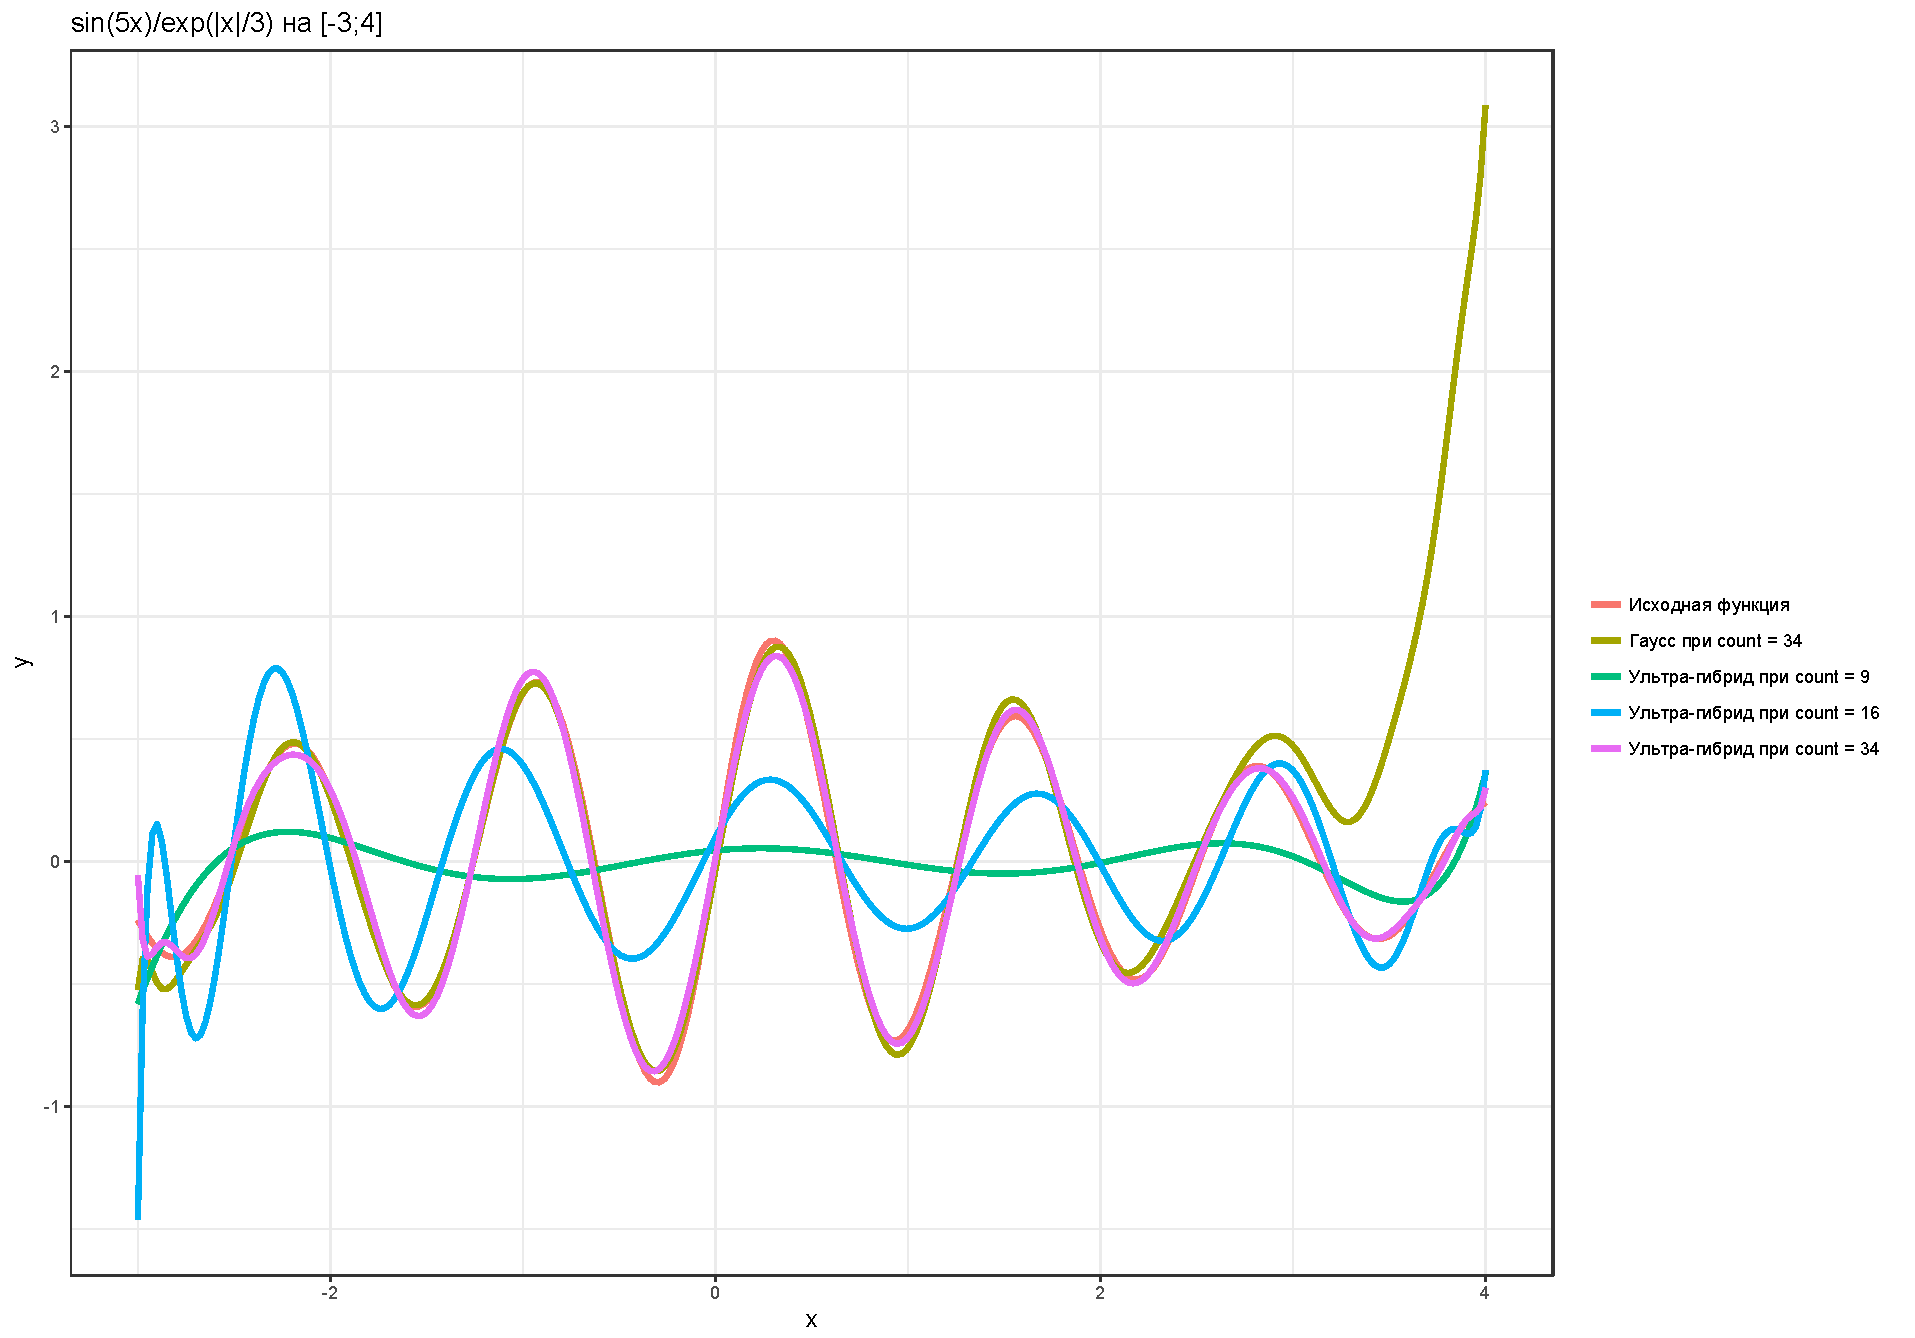
\includegraphics[width=0.85\linewidth]{monex.pdf}
}
 \caption{Аппроксимация мономами}
  \label{monex}
\end{figure}

\begin{figure}[h!]
  \noindent\centering{
  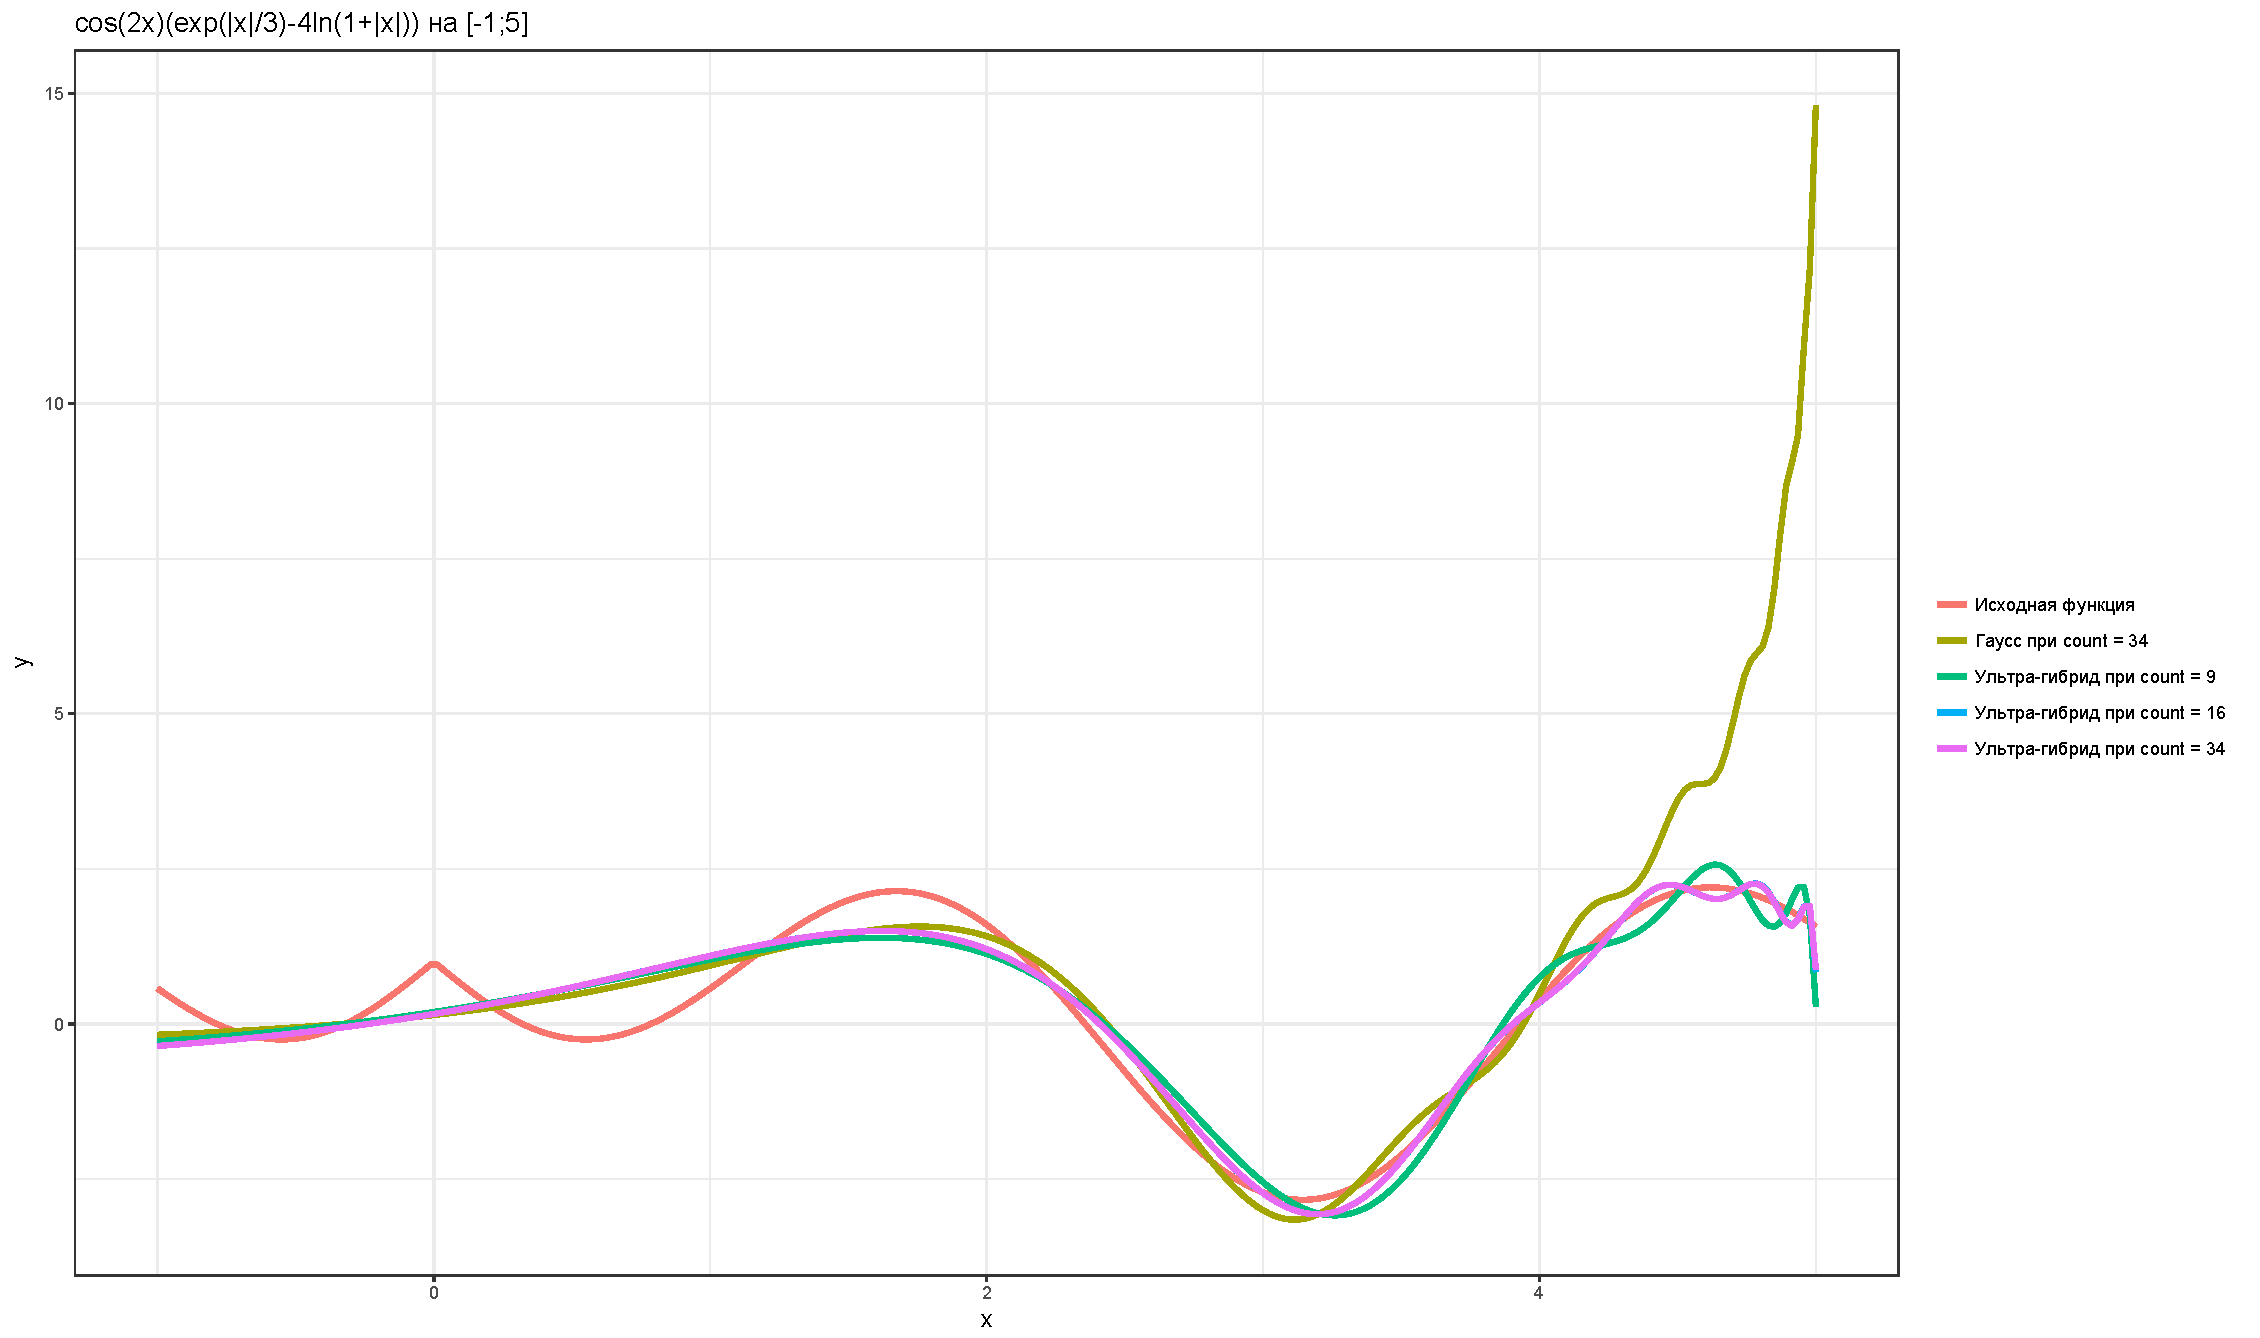
\includegraphics[width=0.85\linewidth]{expex.pdf}
}
 \caption{Аппроксимация экспонентами}
  \label{expex}
\end{figure}

\begin{figure}[h!]
    \noindent\centering{
    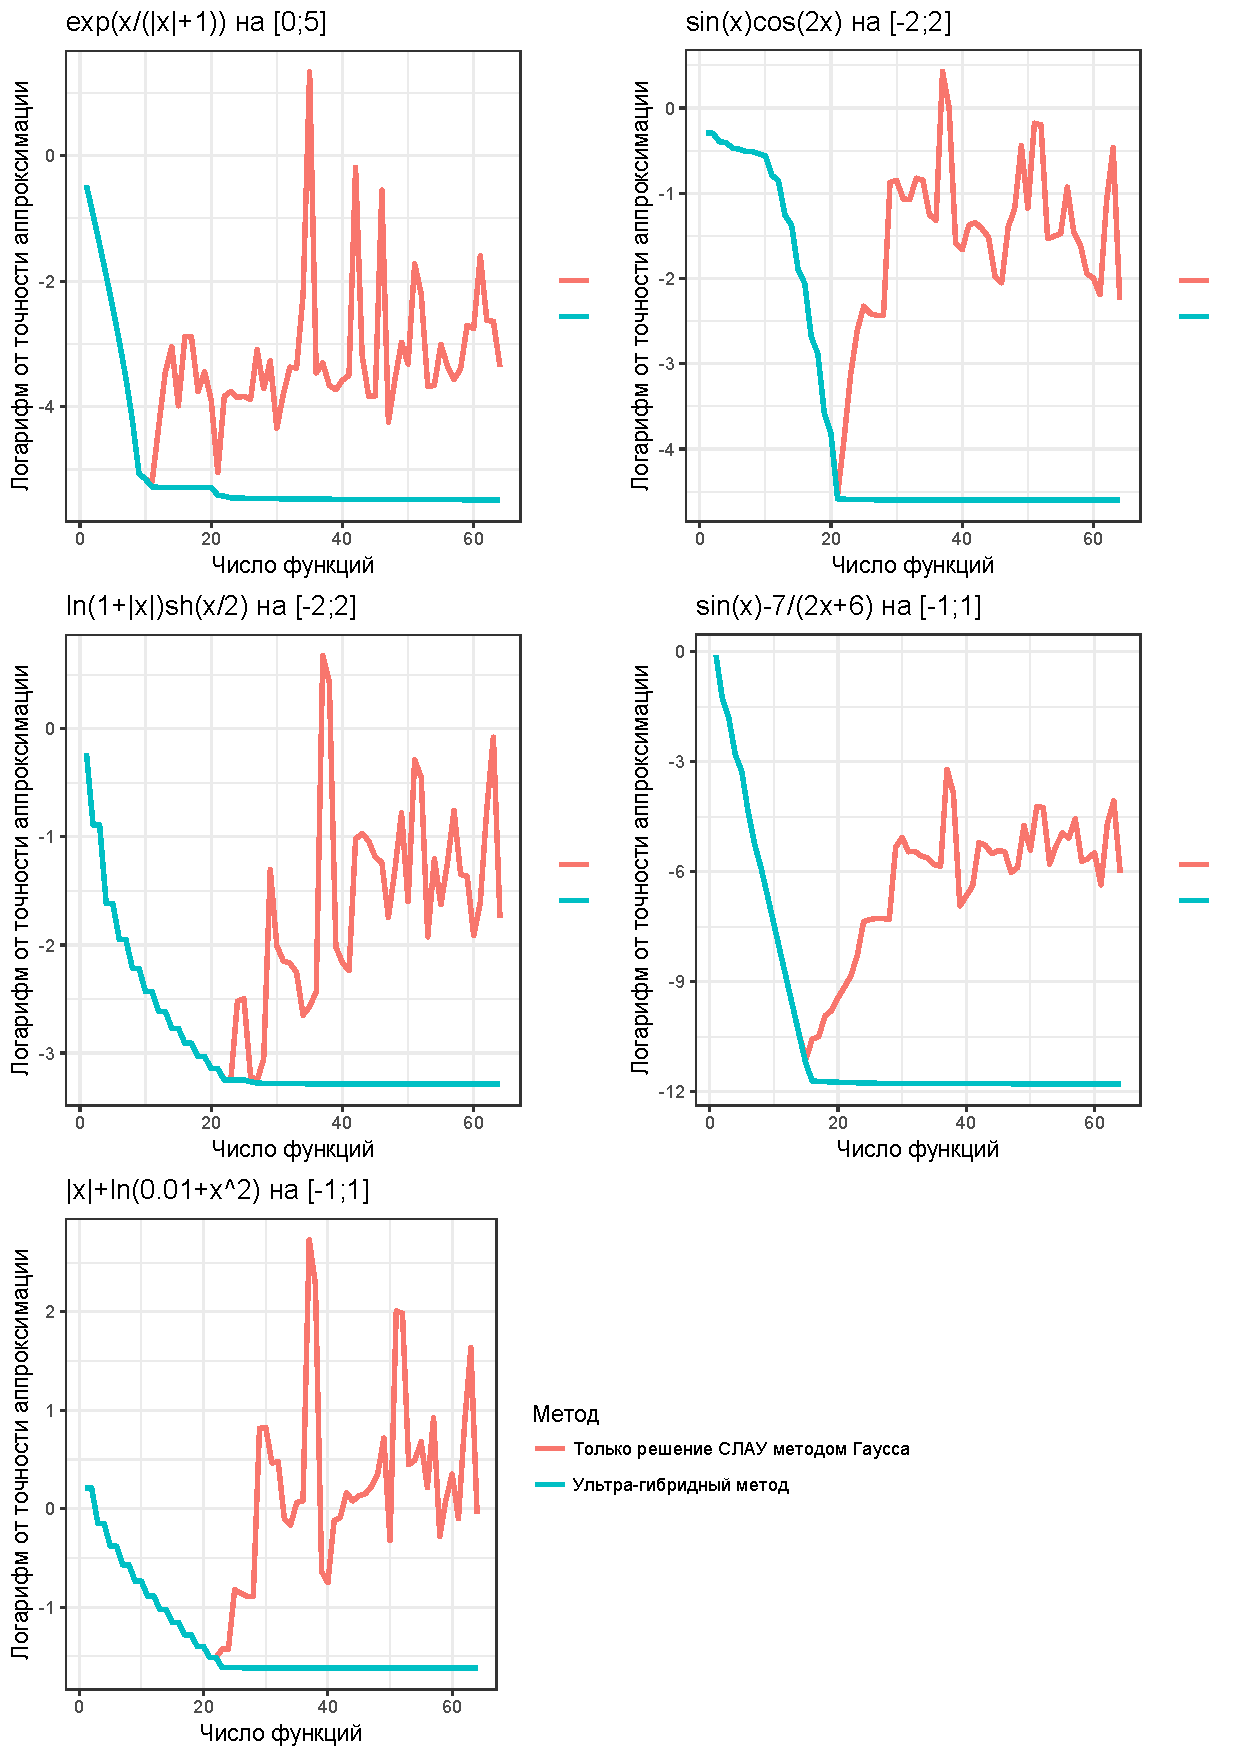
\includegraphics[width=0.9\linewidth]{mon.pdf}
  }
   \caption{Аппроксимация мономами}
    \label{mon}
\end{figure} 

\begin{figure}[h!]
    \noindent\centering{
    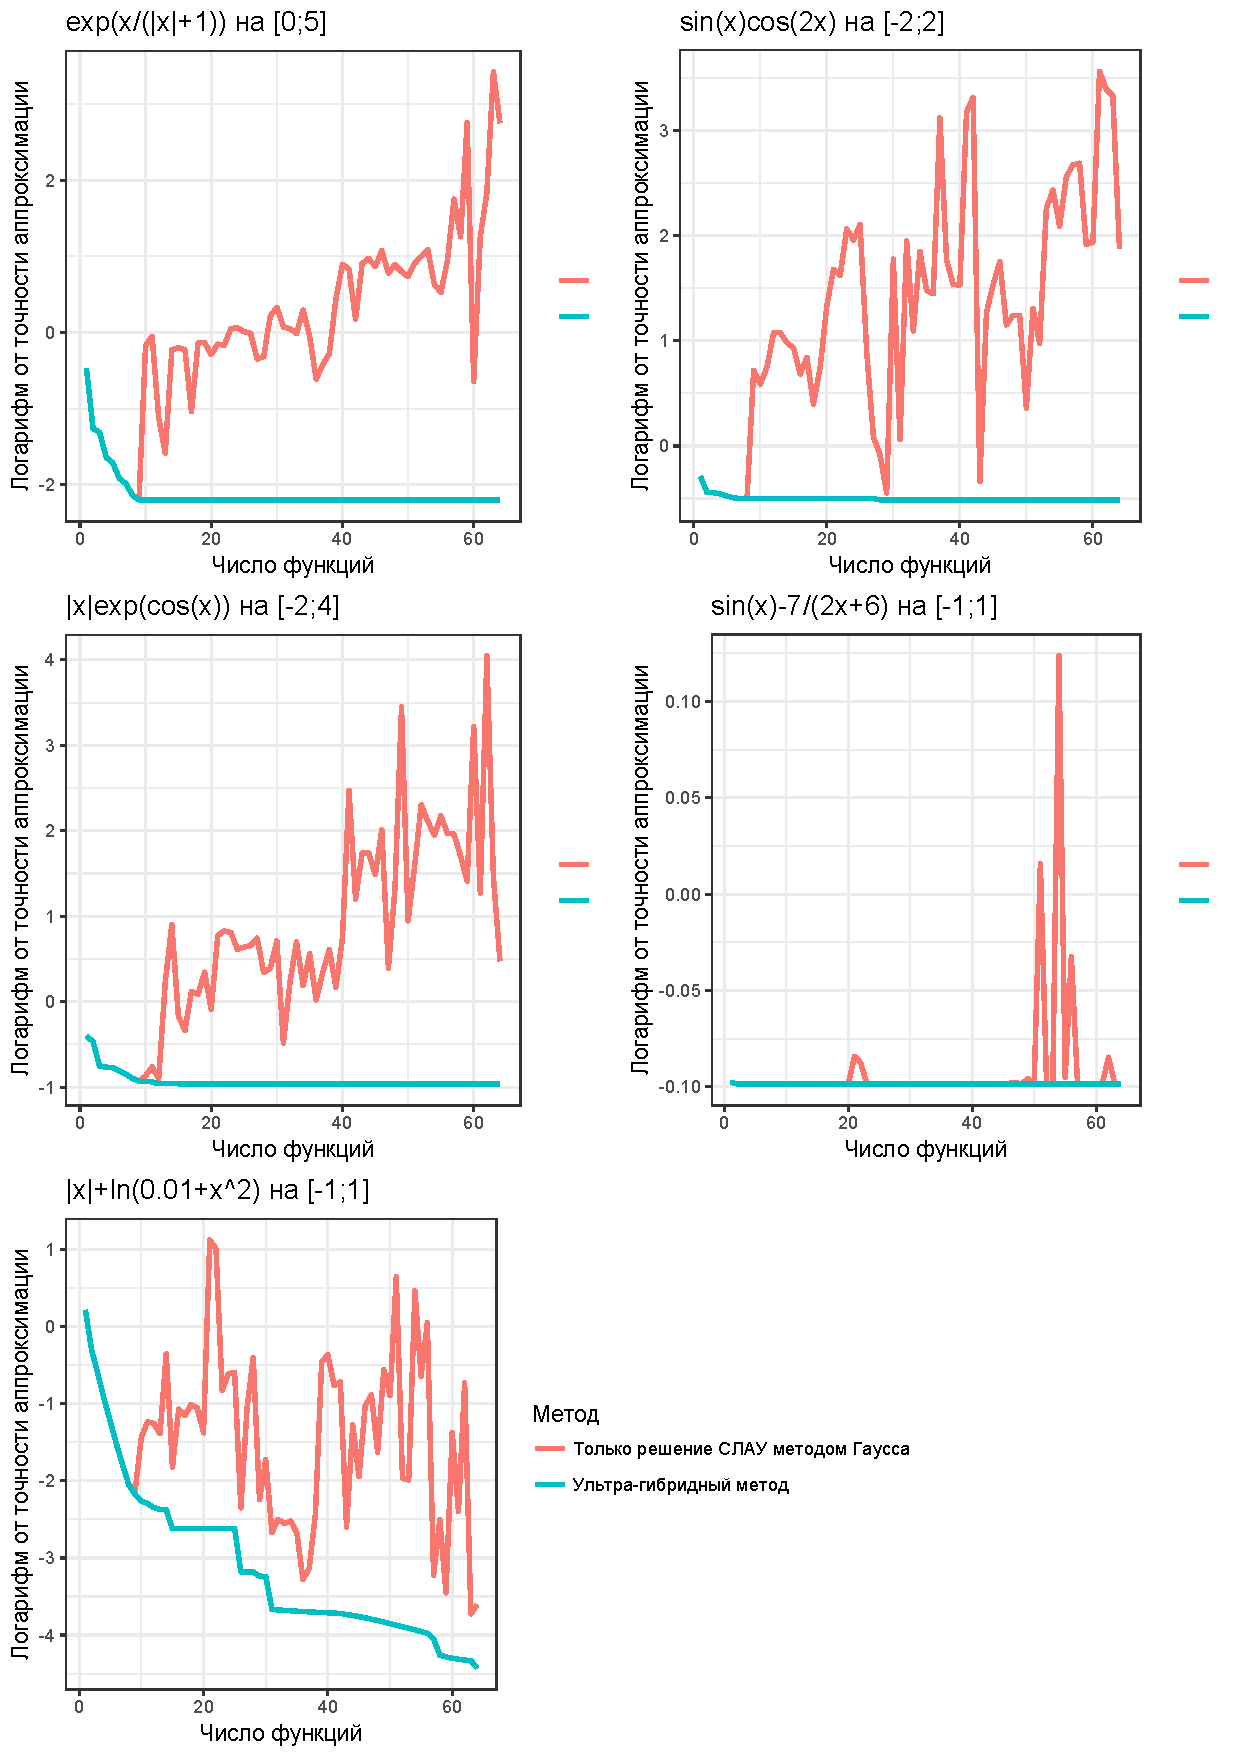
\includegraphics[width=0.9\linewidth]{rat.pdf}
  }
   \caption{Аппроксимация дробями}
    \label{rat}
\end{figure}

\begin{figure}[h!]
    \noindent\centering{
    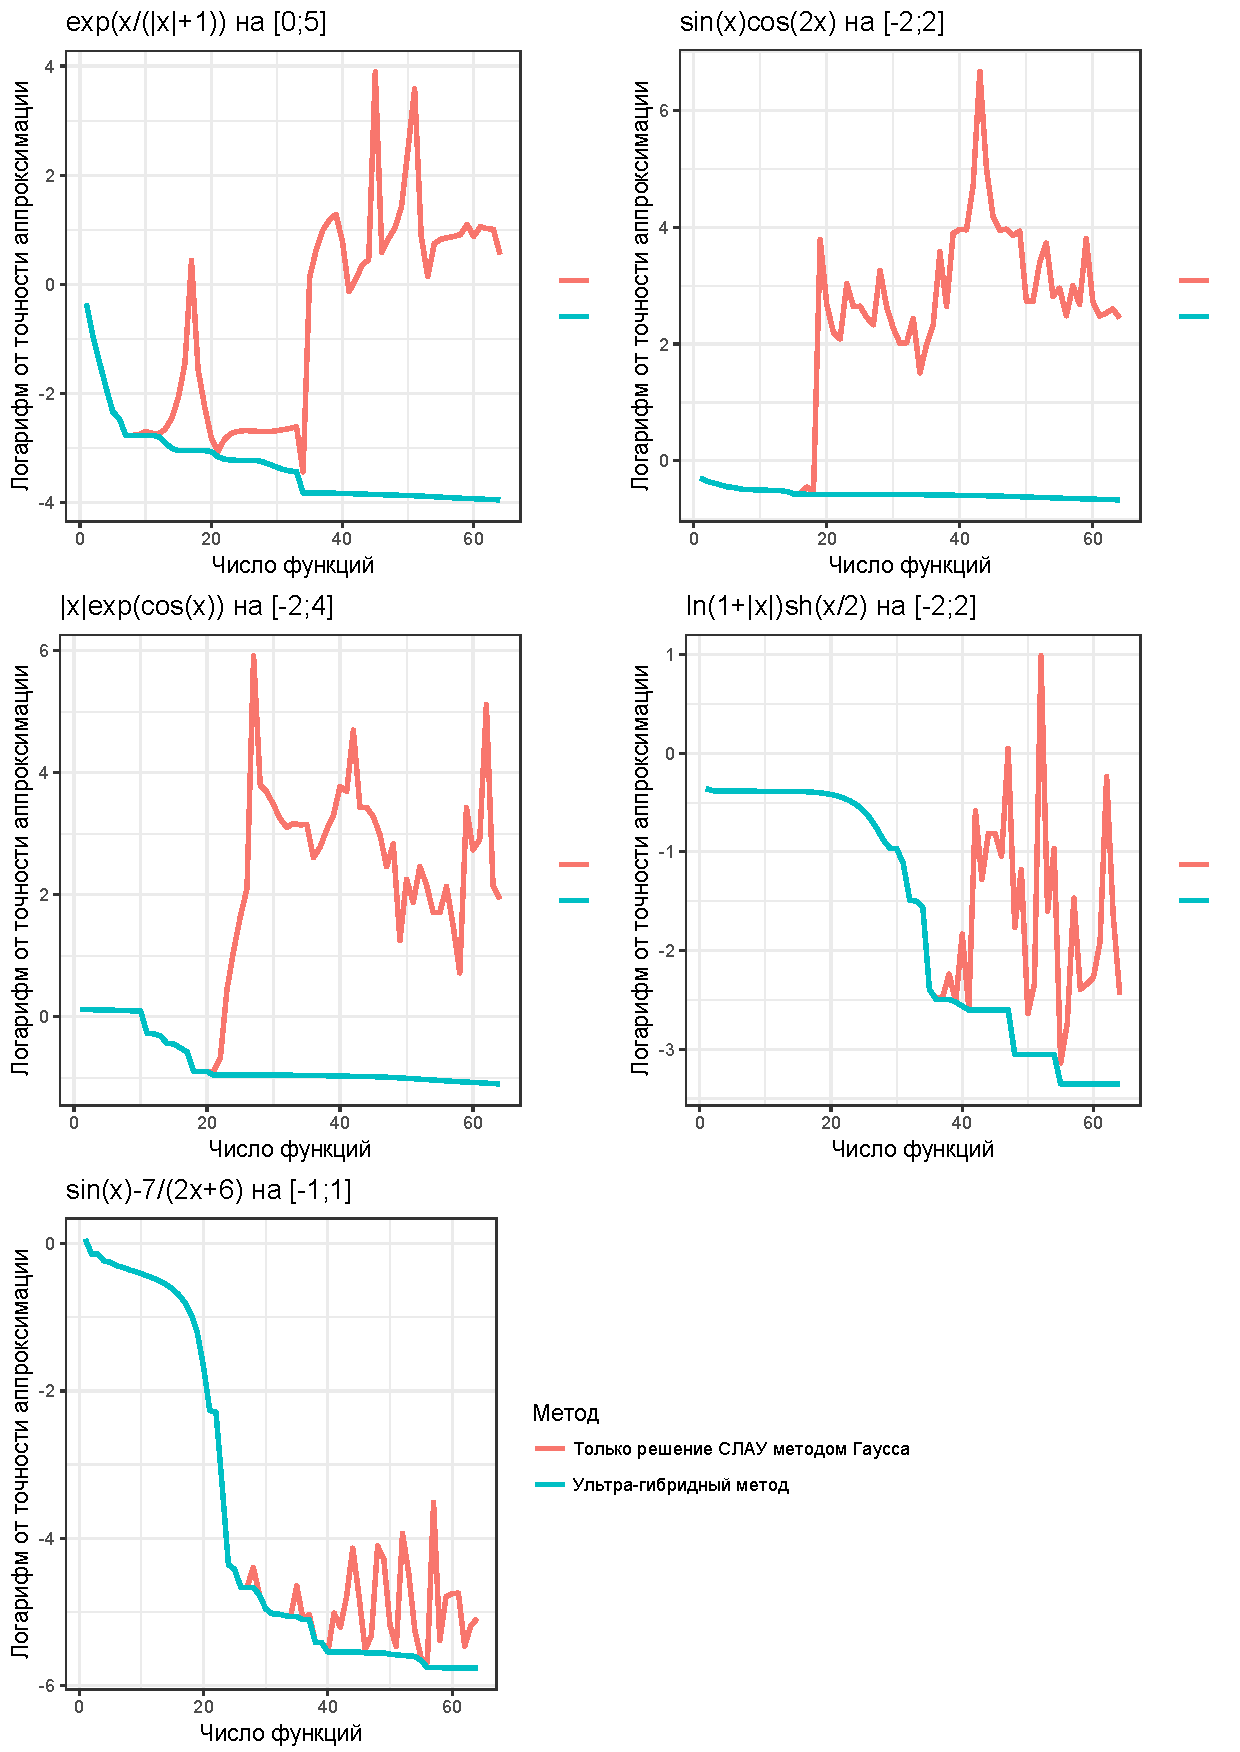
\includegraphics[width=0.9\linewidth]{log.pdf}
  }
   \caption{Аппроксимация логарифмами}
    \label{log}
\end{figure}


Алгоритм не гарантирует нахождения максимально точного решения системы, но гарантирует устойчивое невозрастание невязки при росте размерности системы. Сложность алгоритма равна $O(N^4)$, но это не вносит видимого отрицательного вклада в производительность, поскольку системы с плохо обусловленными матрицами, как правило, не используют слишком большими, вдобавок конкретно в исходной задаче на порядок дольше будут вычисляться коэффициенты СЛАУ.

Также следует отметить, что ещё не встречалось примера, когда ультра-гибрид приводил к значительно более точной аппроксимации в сравнении с классическим вариантом при наименьшей невязке (из графиков \ref{mon}-\ref{log} видно, что минимальное значение ультра-гибрида не находится значительно ниже минимального значения классического метода). Подлинная ценность ультра-гибрида будет показана позже.

\FloatBarrier 
\subsection{Примеры решения ОЗГ}
В этом разделе приводятся примеры решения ОЗГ для разных областей и плотностей.
В качестве областей брались области, ограниченные кривыми из рисунков (\ref{kvci}) и (\ref{tros}) (названия соответственно CIRCLE, TRIANGLE, SQUARE и EDGE) с той же параметризацией, возможно, слегка подкорректированной для возможности интегрирования описанным ранее методом; радиус кривых по умолчанию равен 0.5.
В качестве граничных функций брались как гармонические, так и негармонические, чтобы продемонстрировать, как метод будет приближённо искать их гармоническую часть и как много найденная часть вносит в саму аппроксимируемую функцию; функции были следующими ($x,y$ --- координаты точки на плоскости, $\alpha$ --- аргумент точки относительно начала координат):
\begin{equation*}
  f_1=x+y,
\end{equation*}
\begin{equation*}
  f_2=\sin (y) \left(e^x+e^{-x}\right),
\end{equation*}
\begin{equation*}
  f_3=3x+6y+\sqrt{x^2+y^2}+\dfrac{1}{2}y^2,
\end{equation*}
\begin{equation*}
  f_4=1.5,
\end{equation*}
\begin{equation*}
  f_5=x^2-y^2,
\end{equation*}
\begin{equation*}
  f_6=f_1(x,y) \cdot e^{x-y}=(x+y)e^{x-y},
\end{equation*}
\begin{equation*}
  f_7=
  \begin{cases}
    -\frac{1}{2},& -\pi \leq \alpha < -\frac{2 \pi}{3} \\
    0,& -\frac{2 \pi}{3} < \alpha \leq -\frac{\pi}{3} \\
    \frac{1}{2},& -\frac{\pi}{3} < \alpha \leq \frac{\pi}{2}  \\
    -\frac{1}{2},&\text{иначе}
  \end{cases},
\end{equation*}
\begin{equation*}
  f_8=f_3+f_7,
\end{equation*}
\begin{equation*}
  f_9= e^x( \cos y +3\sin  y),
\end{equation*}
\begin{equation*}
  f_{10}= \sum_{i=1}^{5} f_i,
\end{equation*}
\begin{equation*}
  f_{11}= -\ln (|x-z_1|).
\end{equation*}

\subsubsection{Пояснения для рисунков}
Контуры из рисунков (\ref{kvci}) и (\ref{tros}) обозначаются за $\partial Q$, $Q$ --- область, ограниченная одним из этих контуров,
$L$ --- подобный $\partial Q$ контур радиуса $r$, причём $Q$ содержится внутри области, им ограниченной. Радиус $r$ может меняться от собственно радиуса $\partial Q$ до некоторого фиксированного значения.

Приближённое значение плотности $\rho$ равно
\begin{equation*}
  \tilde{\rho} = \sum_i c_i \alpha_i,
\end{equation*}
где $\alpha_i$ --- базисный потенциал от $i$-й точки.
Точек $z_i$ выбрано некоторое количество и располагаются они равномерно по кривой $L_p$, подобной $L$, но большего радиуса (Рис. \ref{points2}), с небольшими случайными отклонениями по нормали от $L$.

На кривой $L$ известна функция $V_f(x)=\V{f}$, где $f$ --- одна из перечисленных ранее тестовых функций.
Тогда коэффициенты $c_i$ из $\tilde{\rho}$ находятся как компоненты решения задачи минимизации:
\begin{equation*}
  F(c_1,\dots,c_i,\dots,c_n)=||V_f-V_{\tilde{\rho} } ||_{L_2(L)}\rightarrow \min.
\end{equation*}

Значение $||V_f-V_{\tilde{\rho} } ||_{L_2(L)}$ есть точность аппроксимации потенциала на $L$.
Значение $||\rho-\tilde{\rho} ||_{L_2(Q)}$ есть точность аппроксимации плотности на области $Q$.
Цель метода --- осуществить аппроксимацию на $Q$.

\subsubsection{2D-графики}
По известному алгоритму для разных областей $Q$ и разных плотностей $\rho=f_i,i=1,2,\dots,10$ были найдены приближённые плотности $\tilde{\rho}$.
На следующих графиках (рисунки \ref{gbeg}-\ref{hexampl}) показаны функции $\rho, \tilde{\rho}$ (плотности) и $V_{\rho},V_{\tilde{\rho}}$ (исходники) на кривых $L$, графики рисуются по отрезку параметризации $L$, число базисных потенциалов $n$ зафиксировано.
Под качеством аппроксимации имеются в виду значения $||\rho-\tilde{\rho} ||_{L_2(Q)}$ и $||V_f-V_{\tilde{\rho} } ||_{L_2(L)}$; в скобках обозначены те же значения для случая, когда $L$ совпадает с $\partial Q$ (когда радиус этих двух контуров одинаков).

\begin{figure}[h] 
  \center{\begin{minipage}[h]{\linewidth} 
  \center{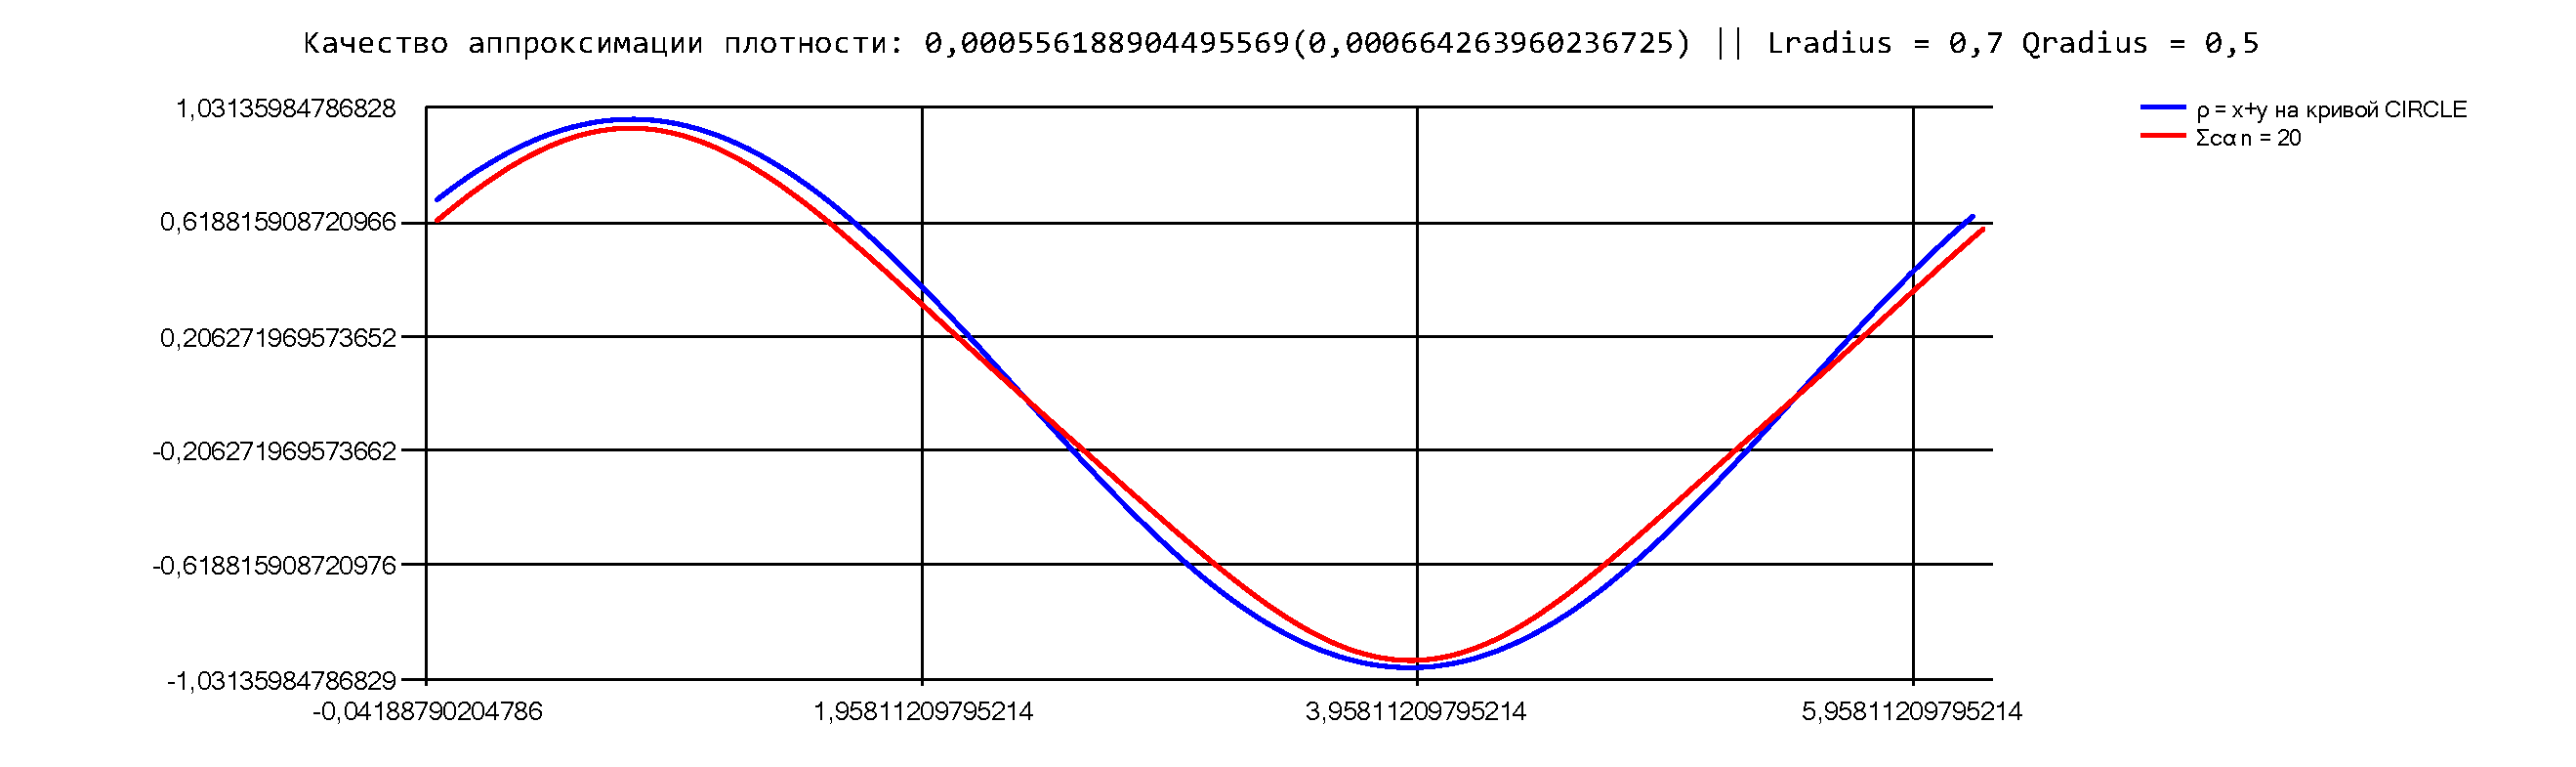
\includegraphics[width=0.8\linewidth]{d1.pdf} \\ для плотности} 
  \end{minipage}} 
  \vfill 
  \center{\begin{minipage}[h]{\linewidth} 
  \center{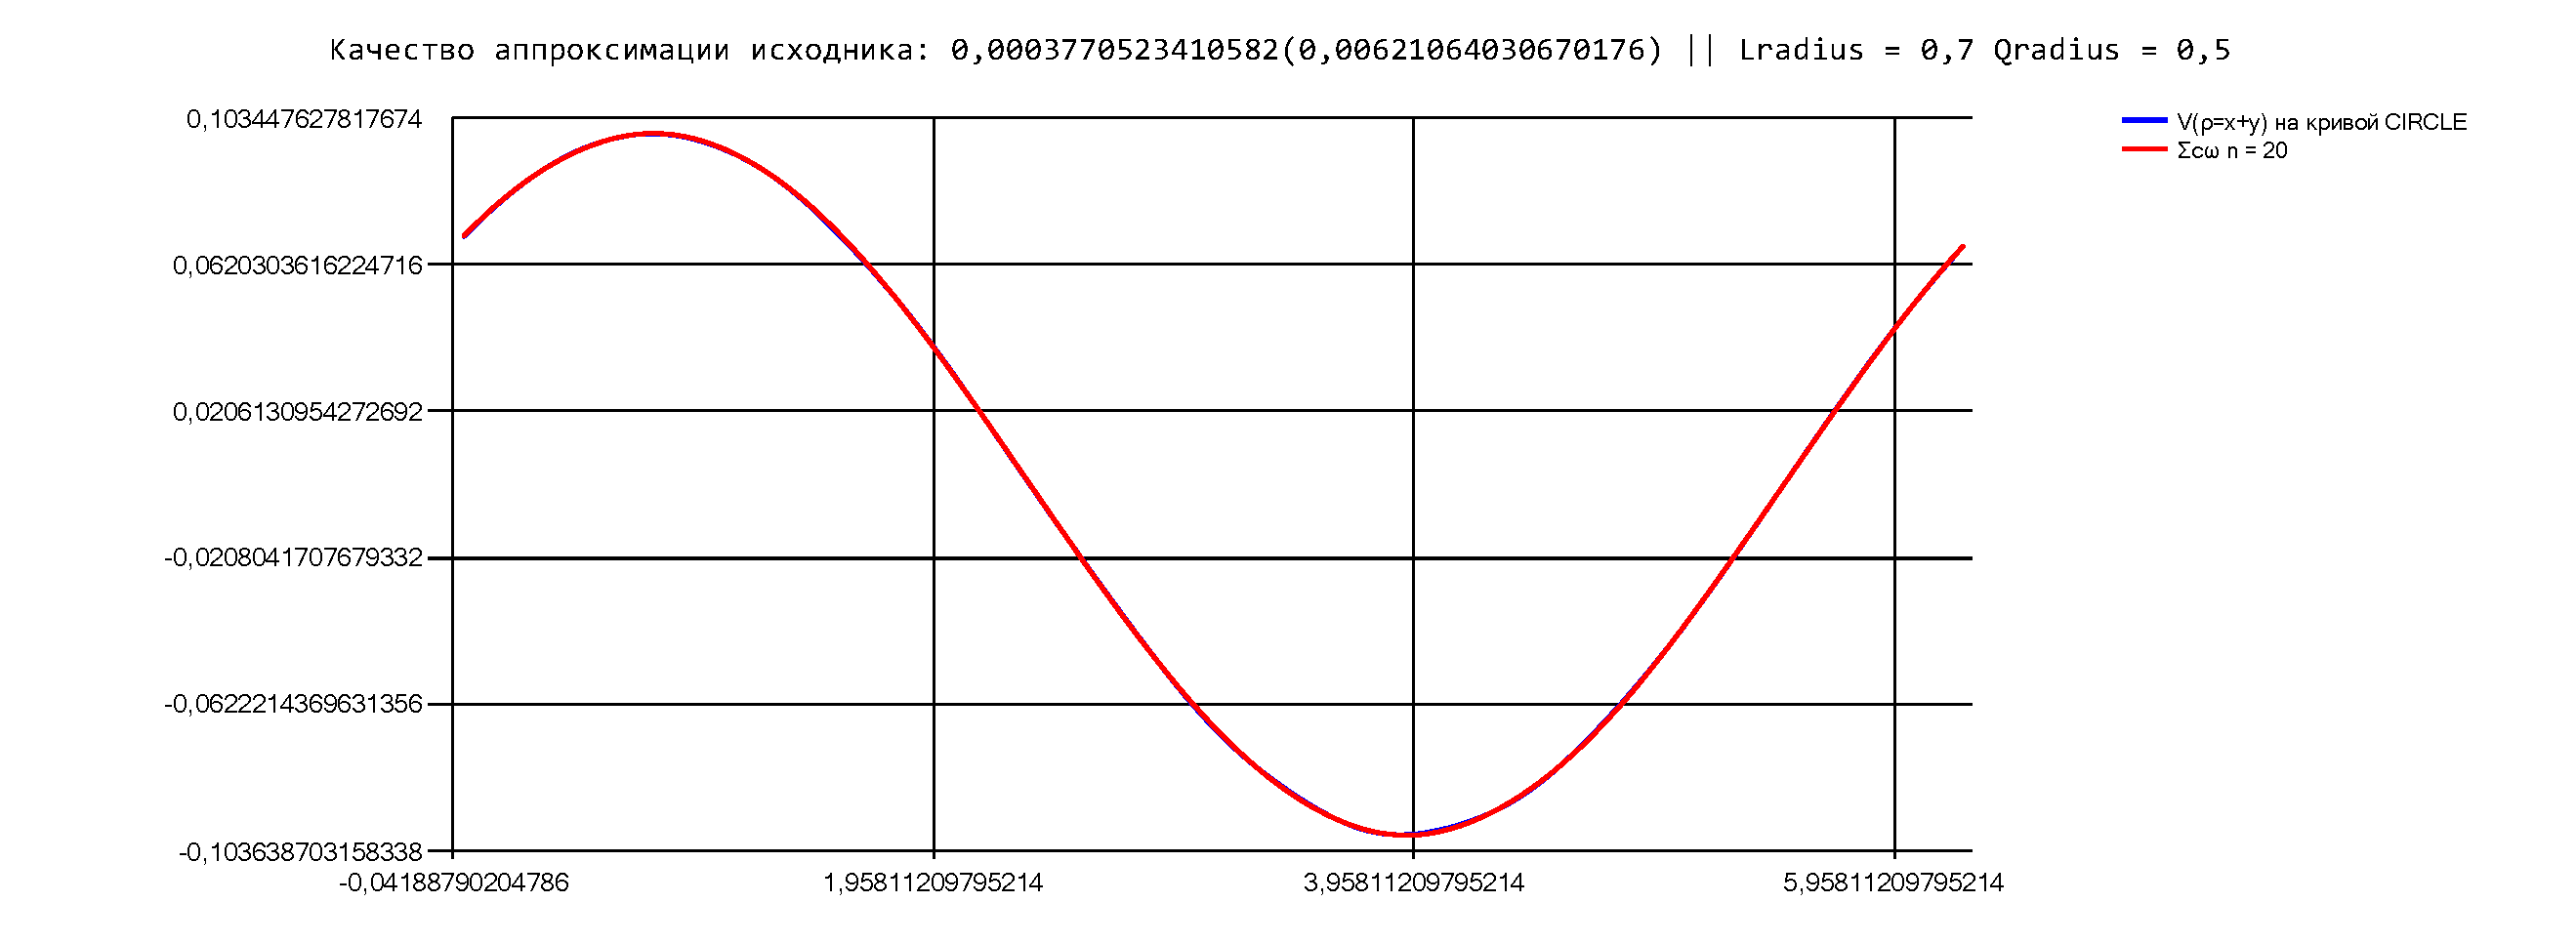
\includegraphics[width=0.8\linewidth]{v1.pdf} \\ для потенциала} 
  \end{minipage}} 
  \caption{Один из результатов работы метода} 
  \label{gbeg} 
  \end{figure}

  \begin{figure}[h] 
    \center{\begin{minipage}[h]{\linewidth} 
    \center{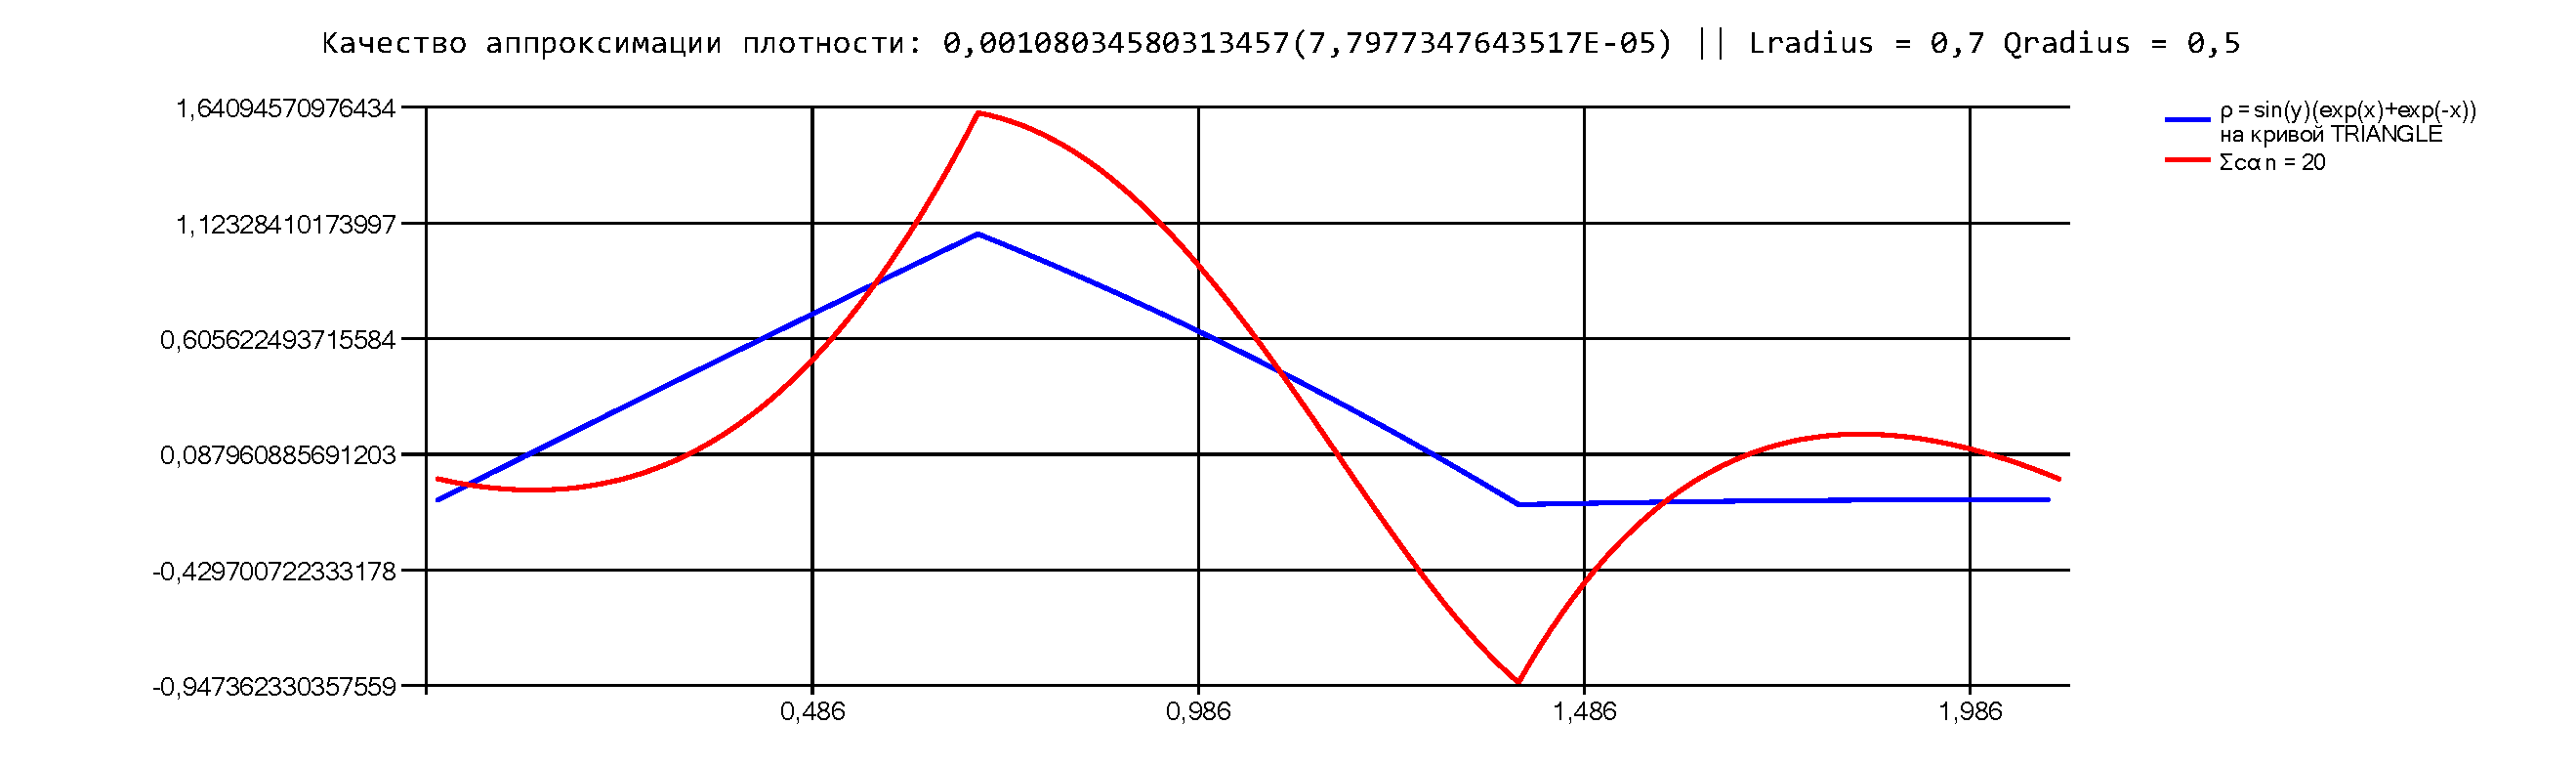
\includegraphics[width=0.8\linewidth]{d2.pdf} \\ для плотности} 
    \end{minipage}} 
    \vfill 
    \center{\begin{minipage}[h]{\linewidth} 
    \center{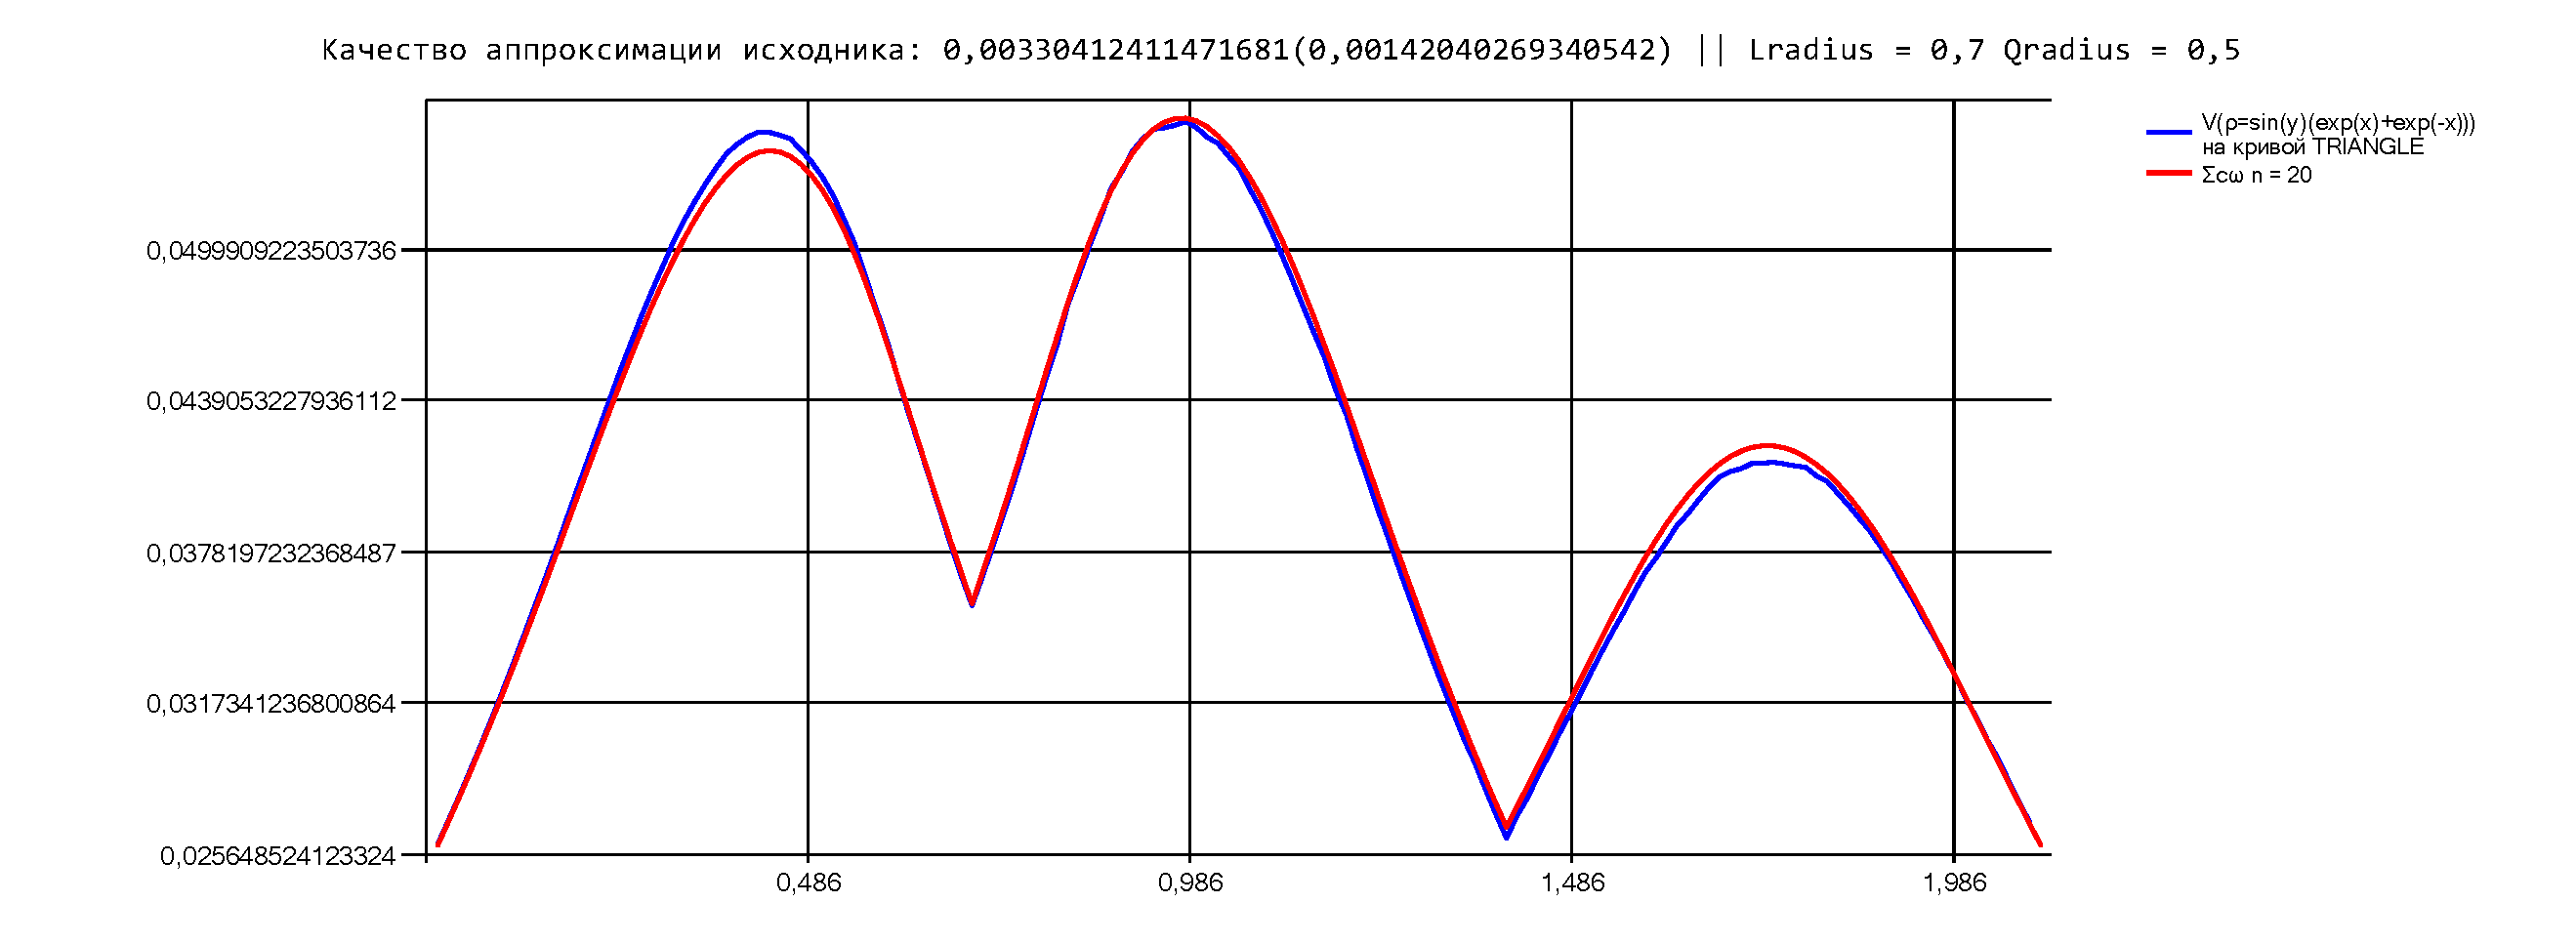
\includegraphics[width=0.8\linewidth]{v2.pdf} \\ для потенциала} 
    \end{minipage}} 
    \caption{Один из результатов работы метода} 
    \label{ris:image1} 
    \end{figure}

    \begin{figure}[h] 
      \center{\begin{minipage}[h]{\linewidth} 
      \center{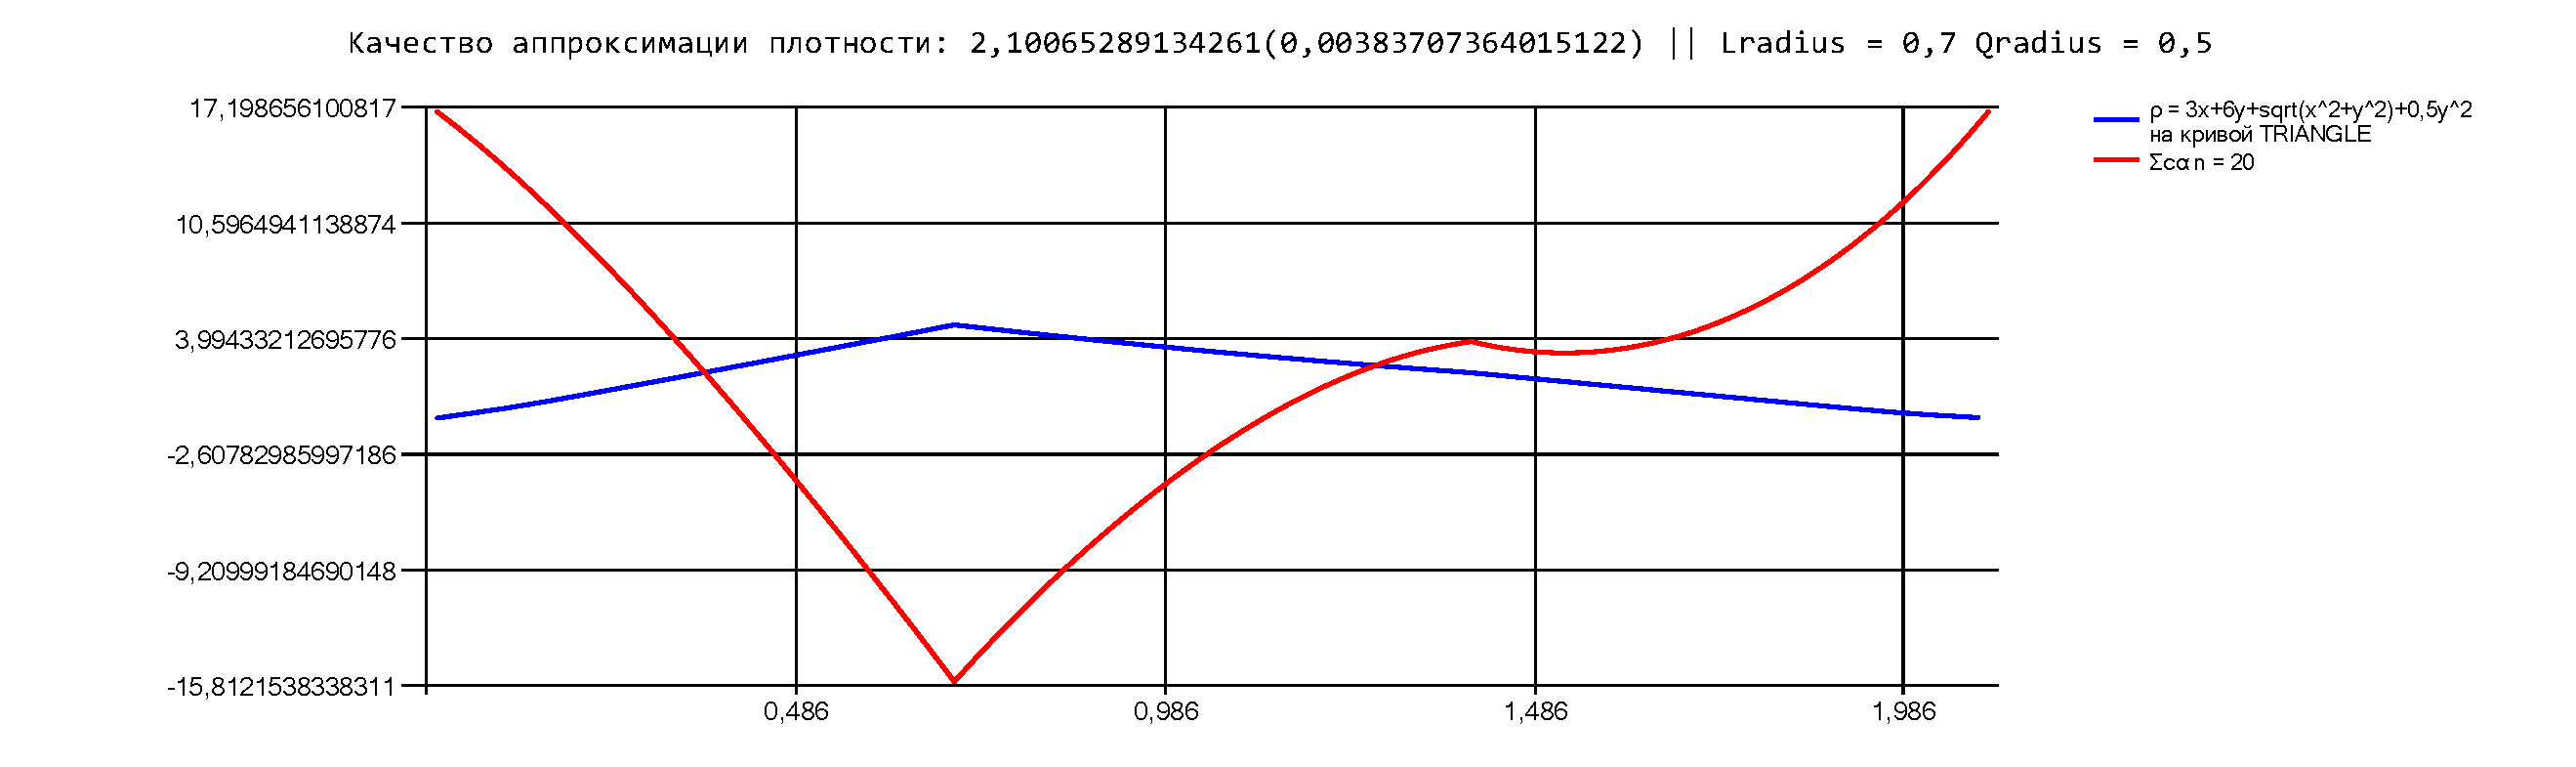
\includegraphics[width=0.8\linewidth]{d3.pdf} \\ для плотности} 
      \end{minipage}} 
      \vfill 
      \center{\begin{minipage}[h]{\linewidth} 
      \center{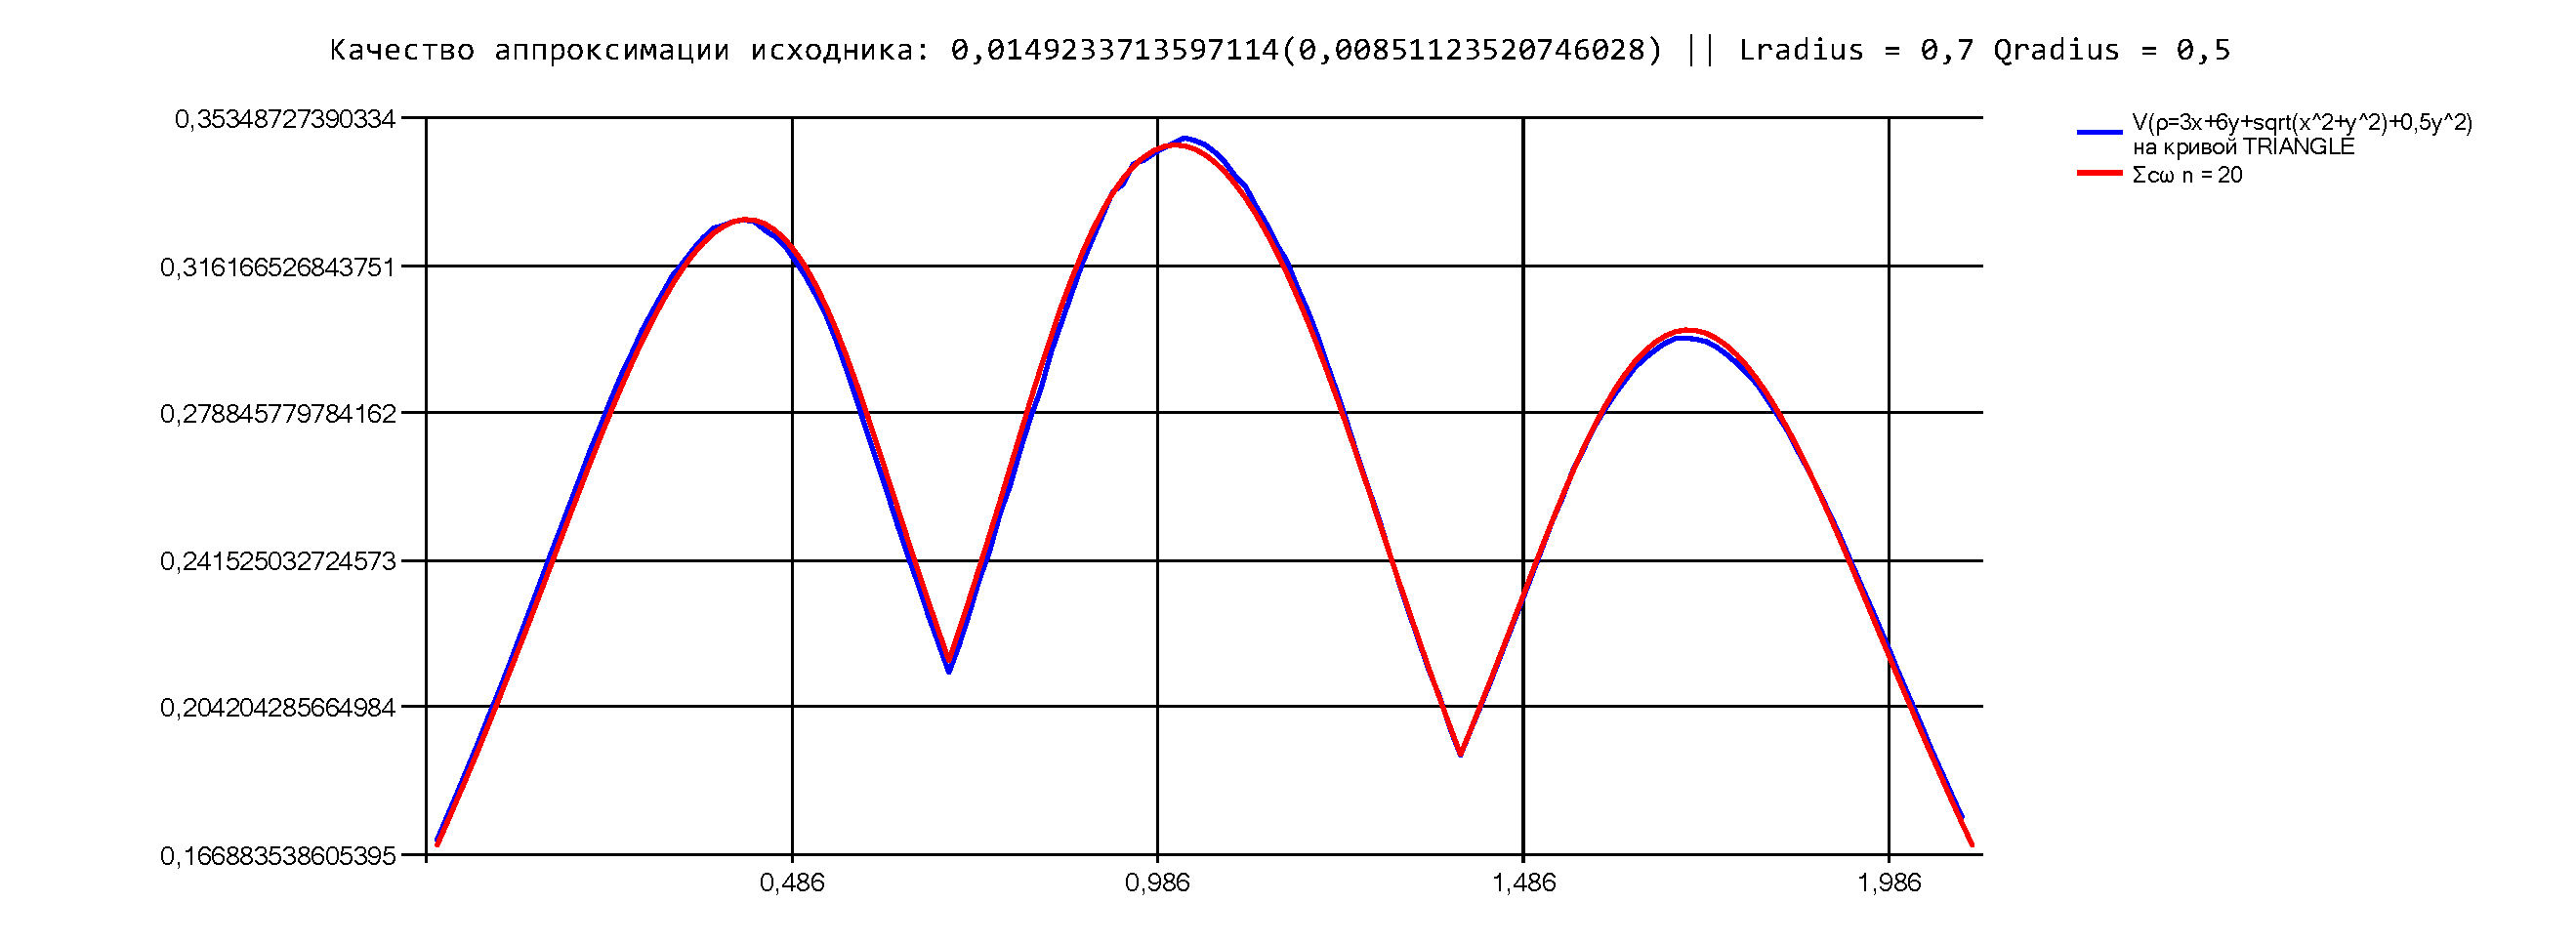
\includegraphics[width=0.8\linewidth]{v3.pdf} \\ для потенциала} 
      \end{minipage}} 
      \caption{Один из результатов работы метода} 
      \label{ris:image1} 
      \end{figure}

      \begin{figure}[h] 
        \center{\begin{minipage}[h]{\linewidth} 
        \center{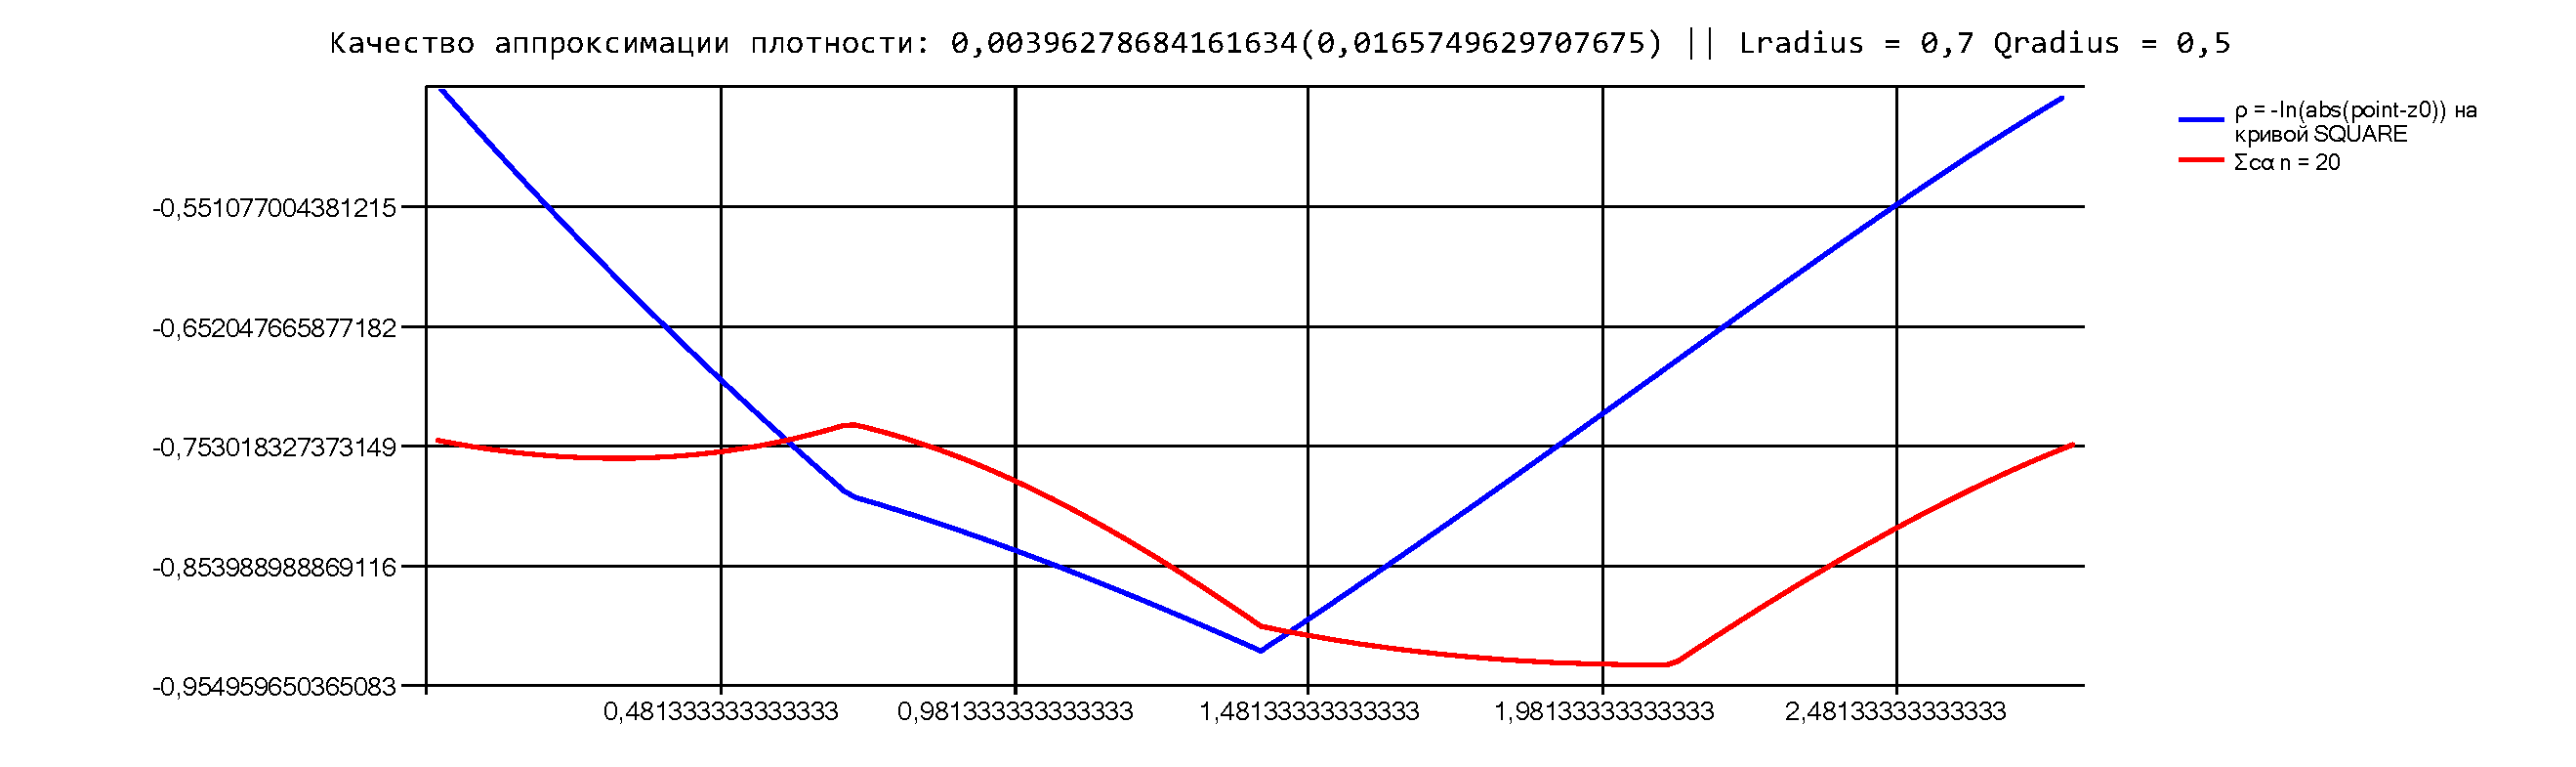
\includegraphics[width=0.8\linewidth]{d4.pdf} \\ для плотности} 
        \end{minipage}} 
        \vfill 
        \center{\begin{minipage}[h]{\linewidth} 
        \center{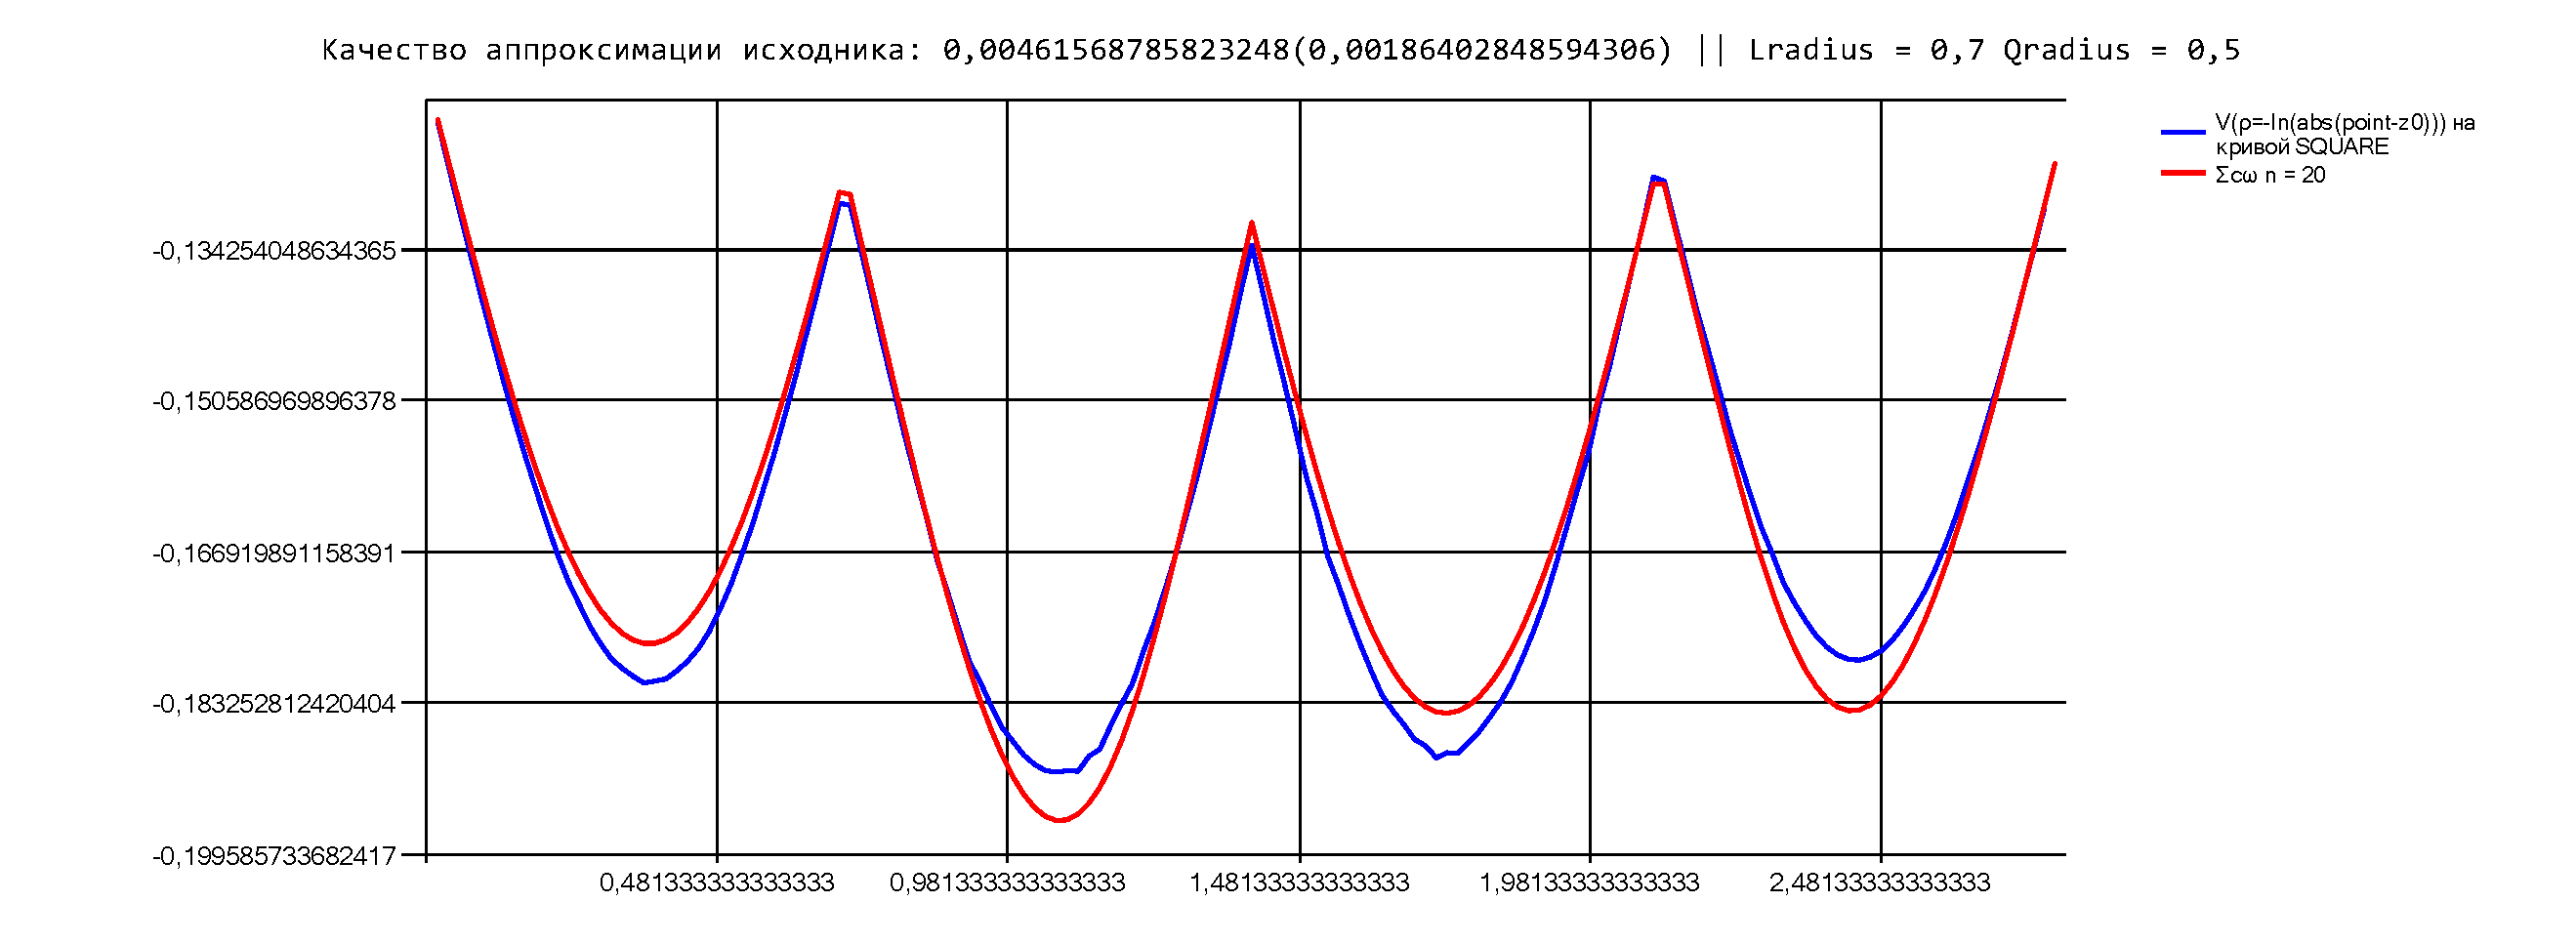
\includegraphics[width=0.8\linewidth]{v4.pdf} \\ для потенциала} 
        \end{minipage}} 
        \caption{Один из результатов работы метода} 
        \label{ris:image1} 
        \end{figure}

        \begin{figure}[h] 
          \center{\begin{minipage}[h]{\linewidth} 
          \center{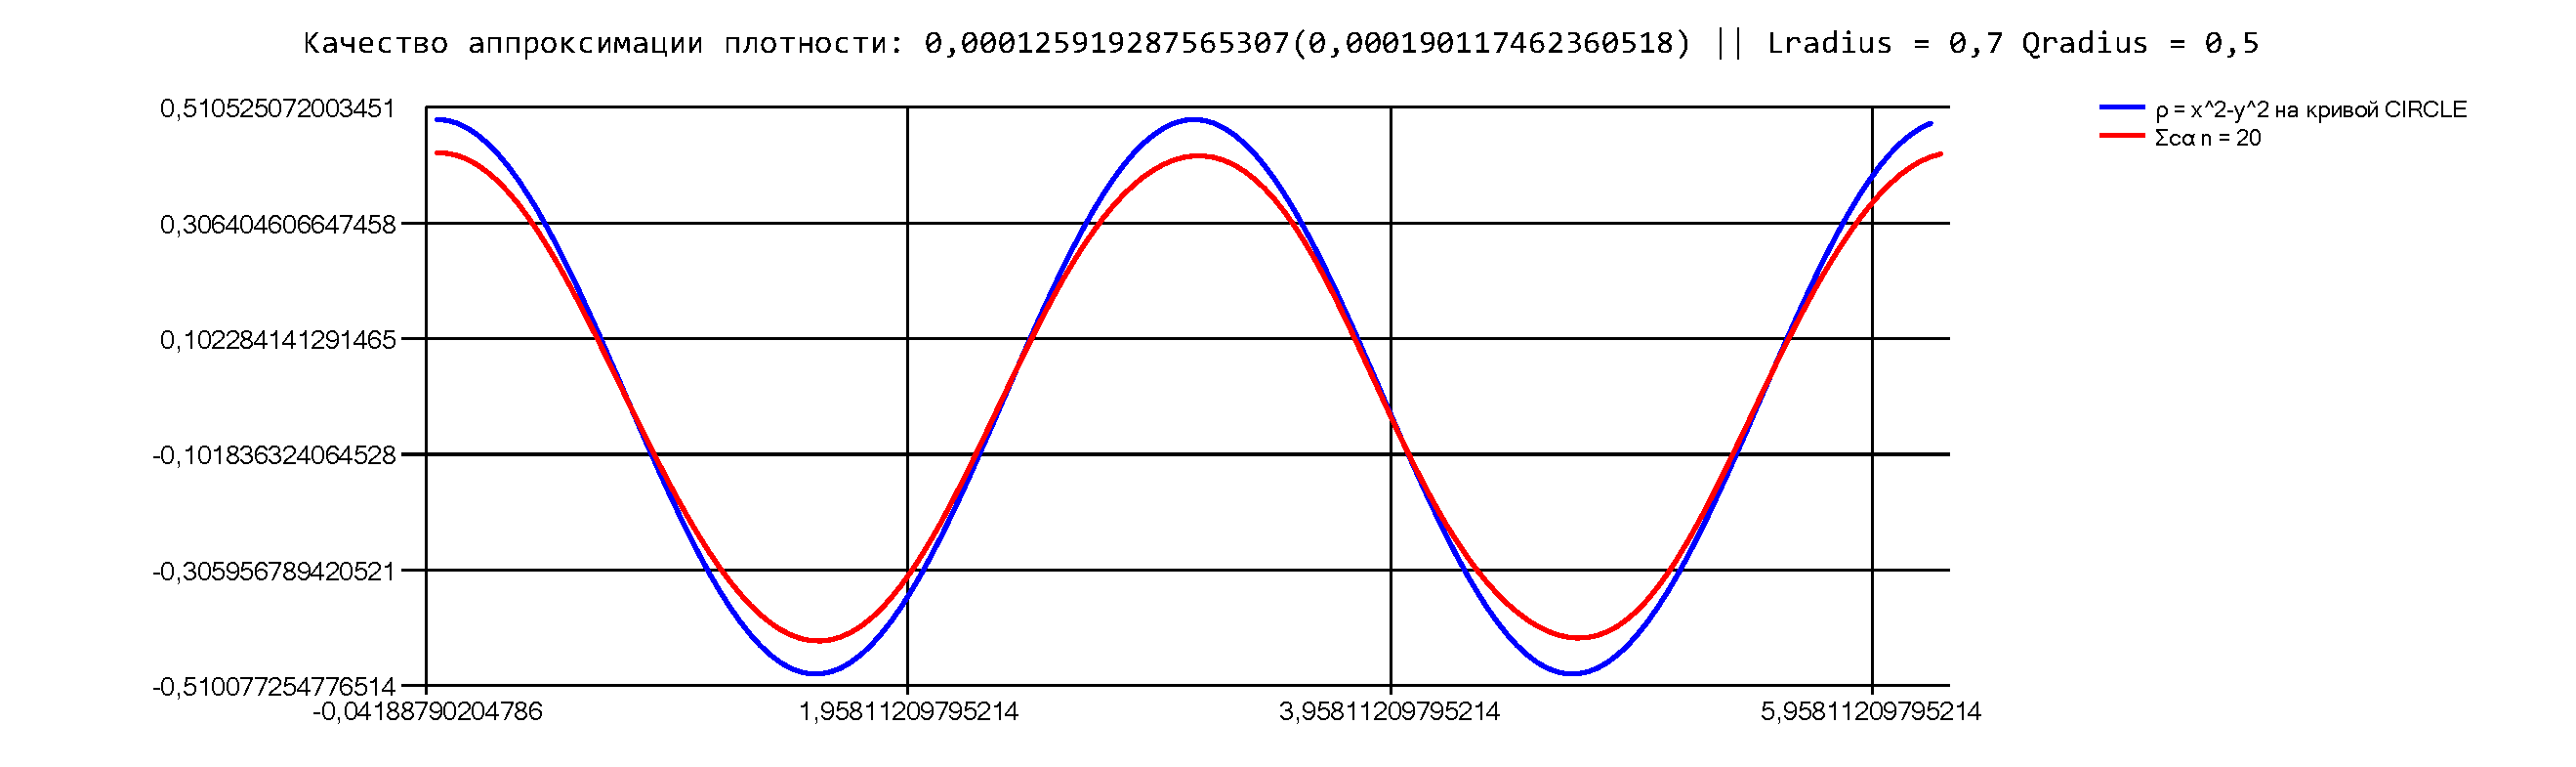
\includegraphics[width=0.8\linewidth]{d5.pdf} \\ для плотности} 
          \end{minipage}} 
          \vfill 
          \center{\begin{minipage}[h]{\linewidth} 
          \center{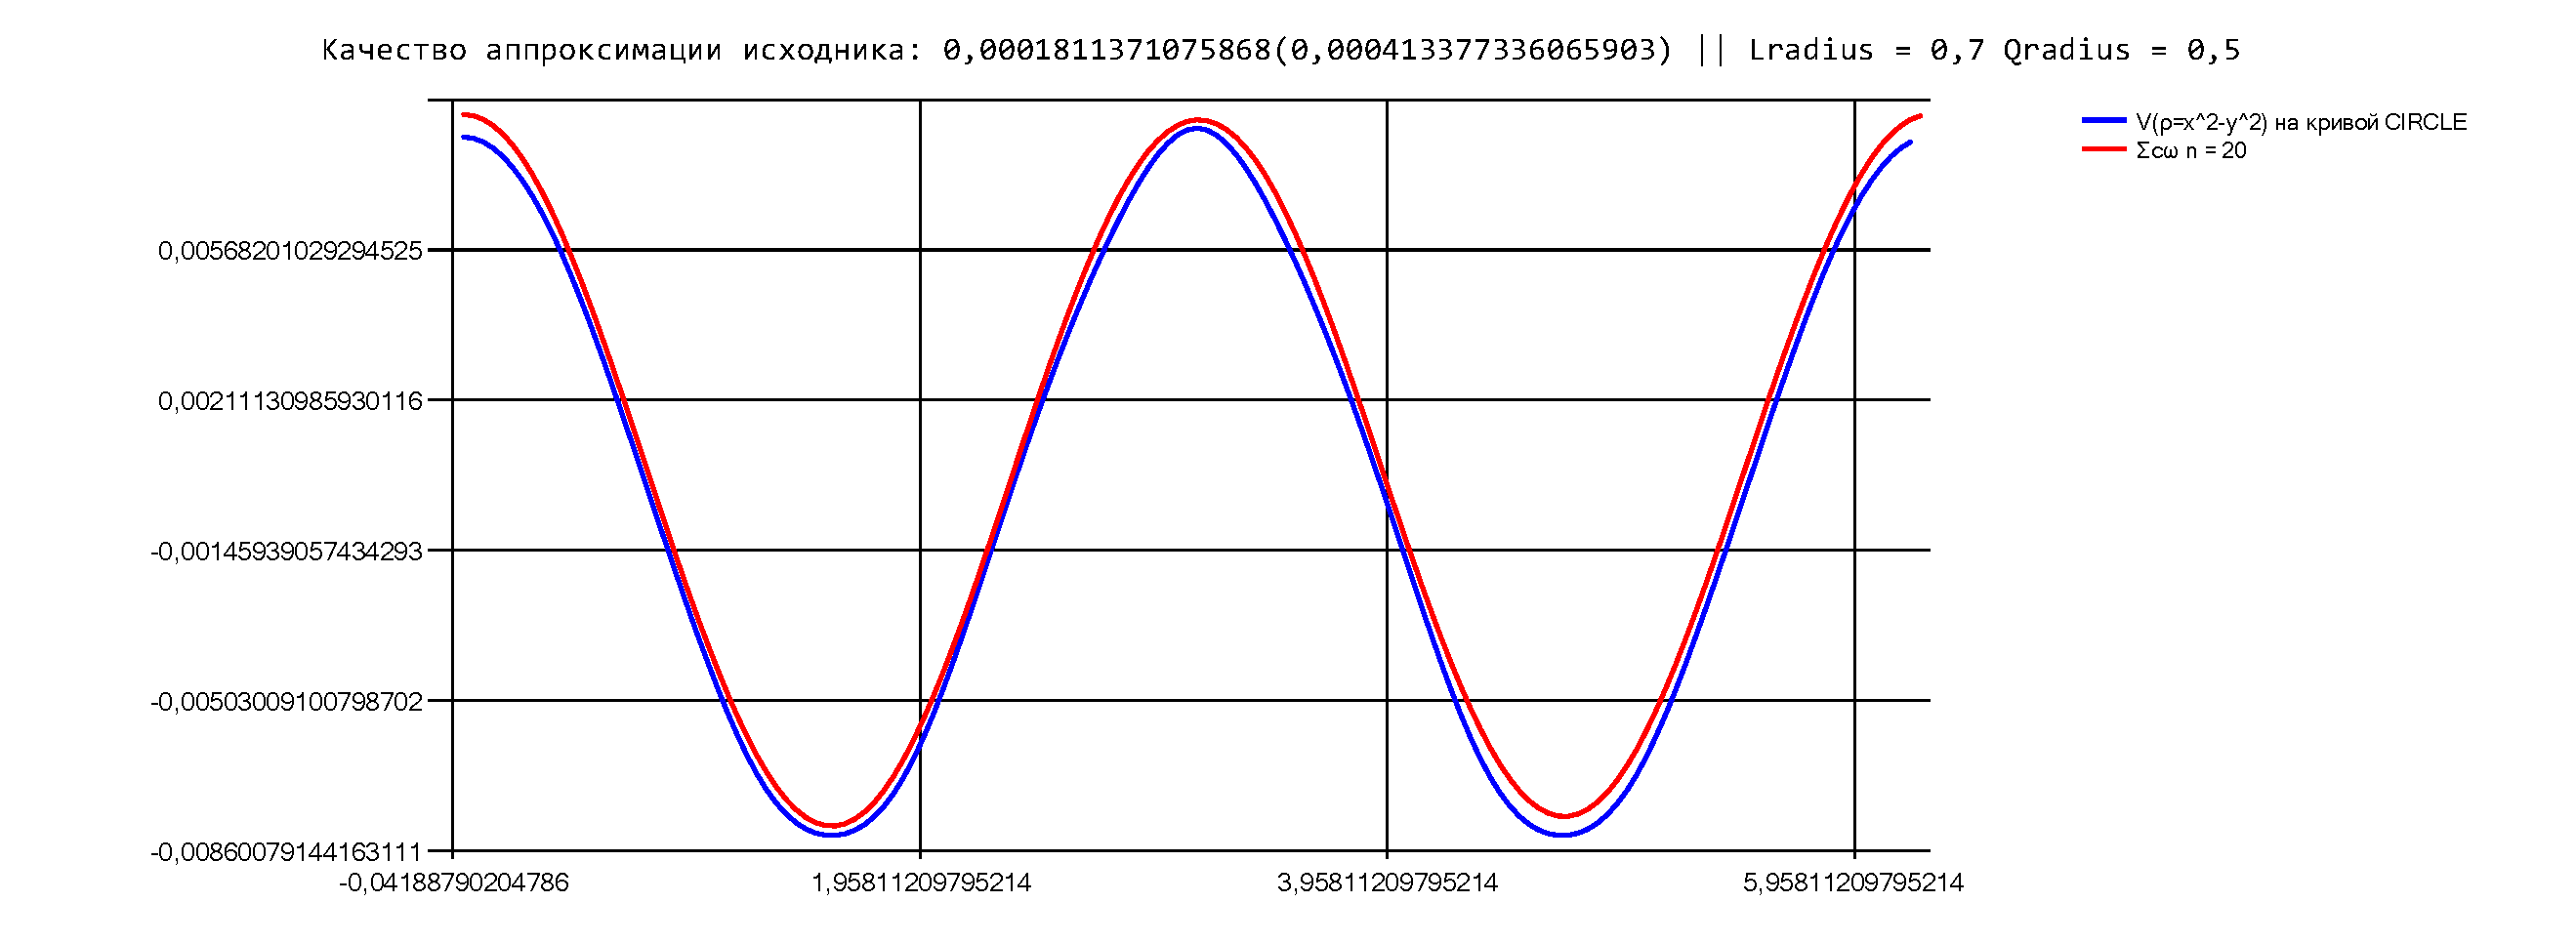
\includegraphics[width=0.8\linewidth]{v5.pdf} \\ для потенциала} 
          \end{minipage}} 
          \caption{Один из результатов работы метода} 
          \label{ris:image1} 
          \end{figure}

          \begin{figure}[h] 
            \center{\begin{minipage}[h]{\linewidth} 
            \center{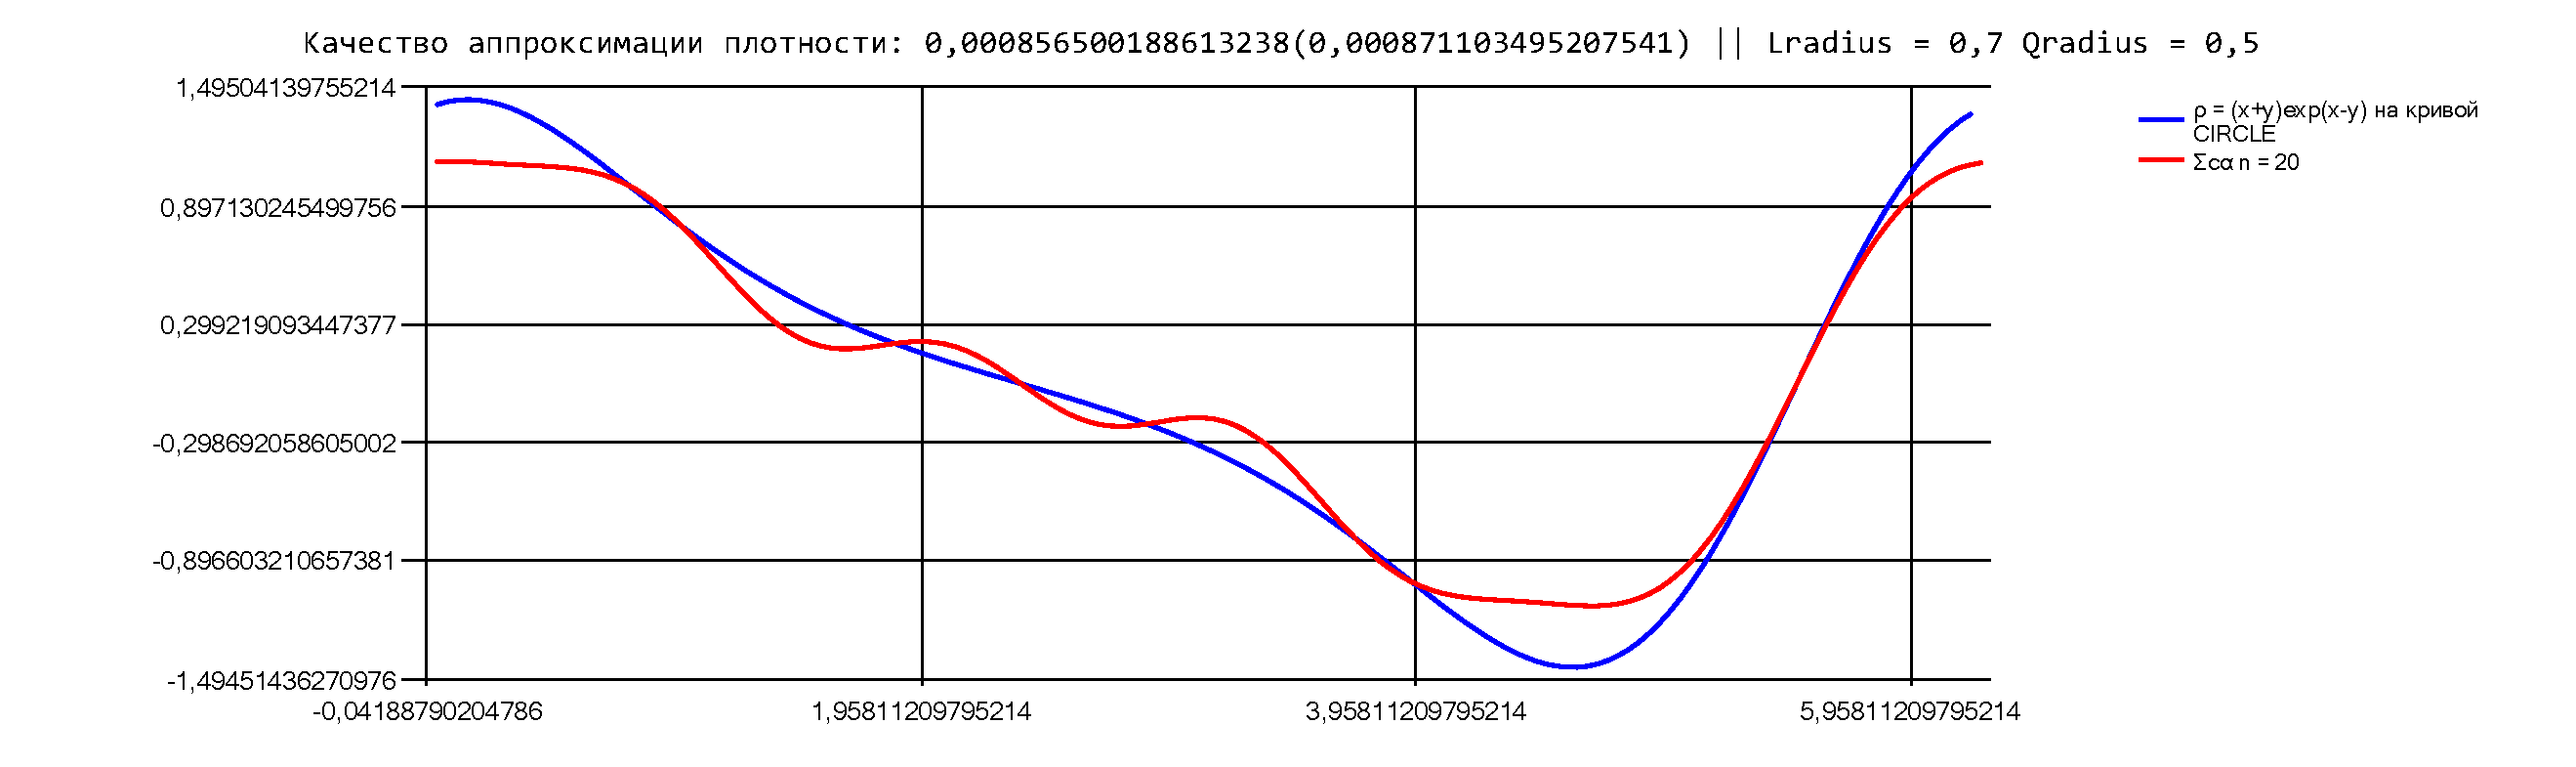
\includegraphics[width=0.8\linewidth]{d6.pdf} \\ для плотности} 
            \end{minipage}} 
            \vfill 
            \center{\begin{minipage}[h]{\linewidth} 
            \center{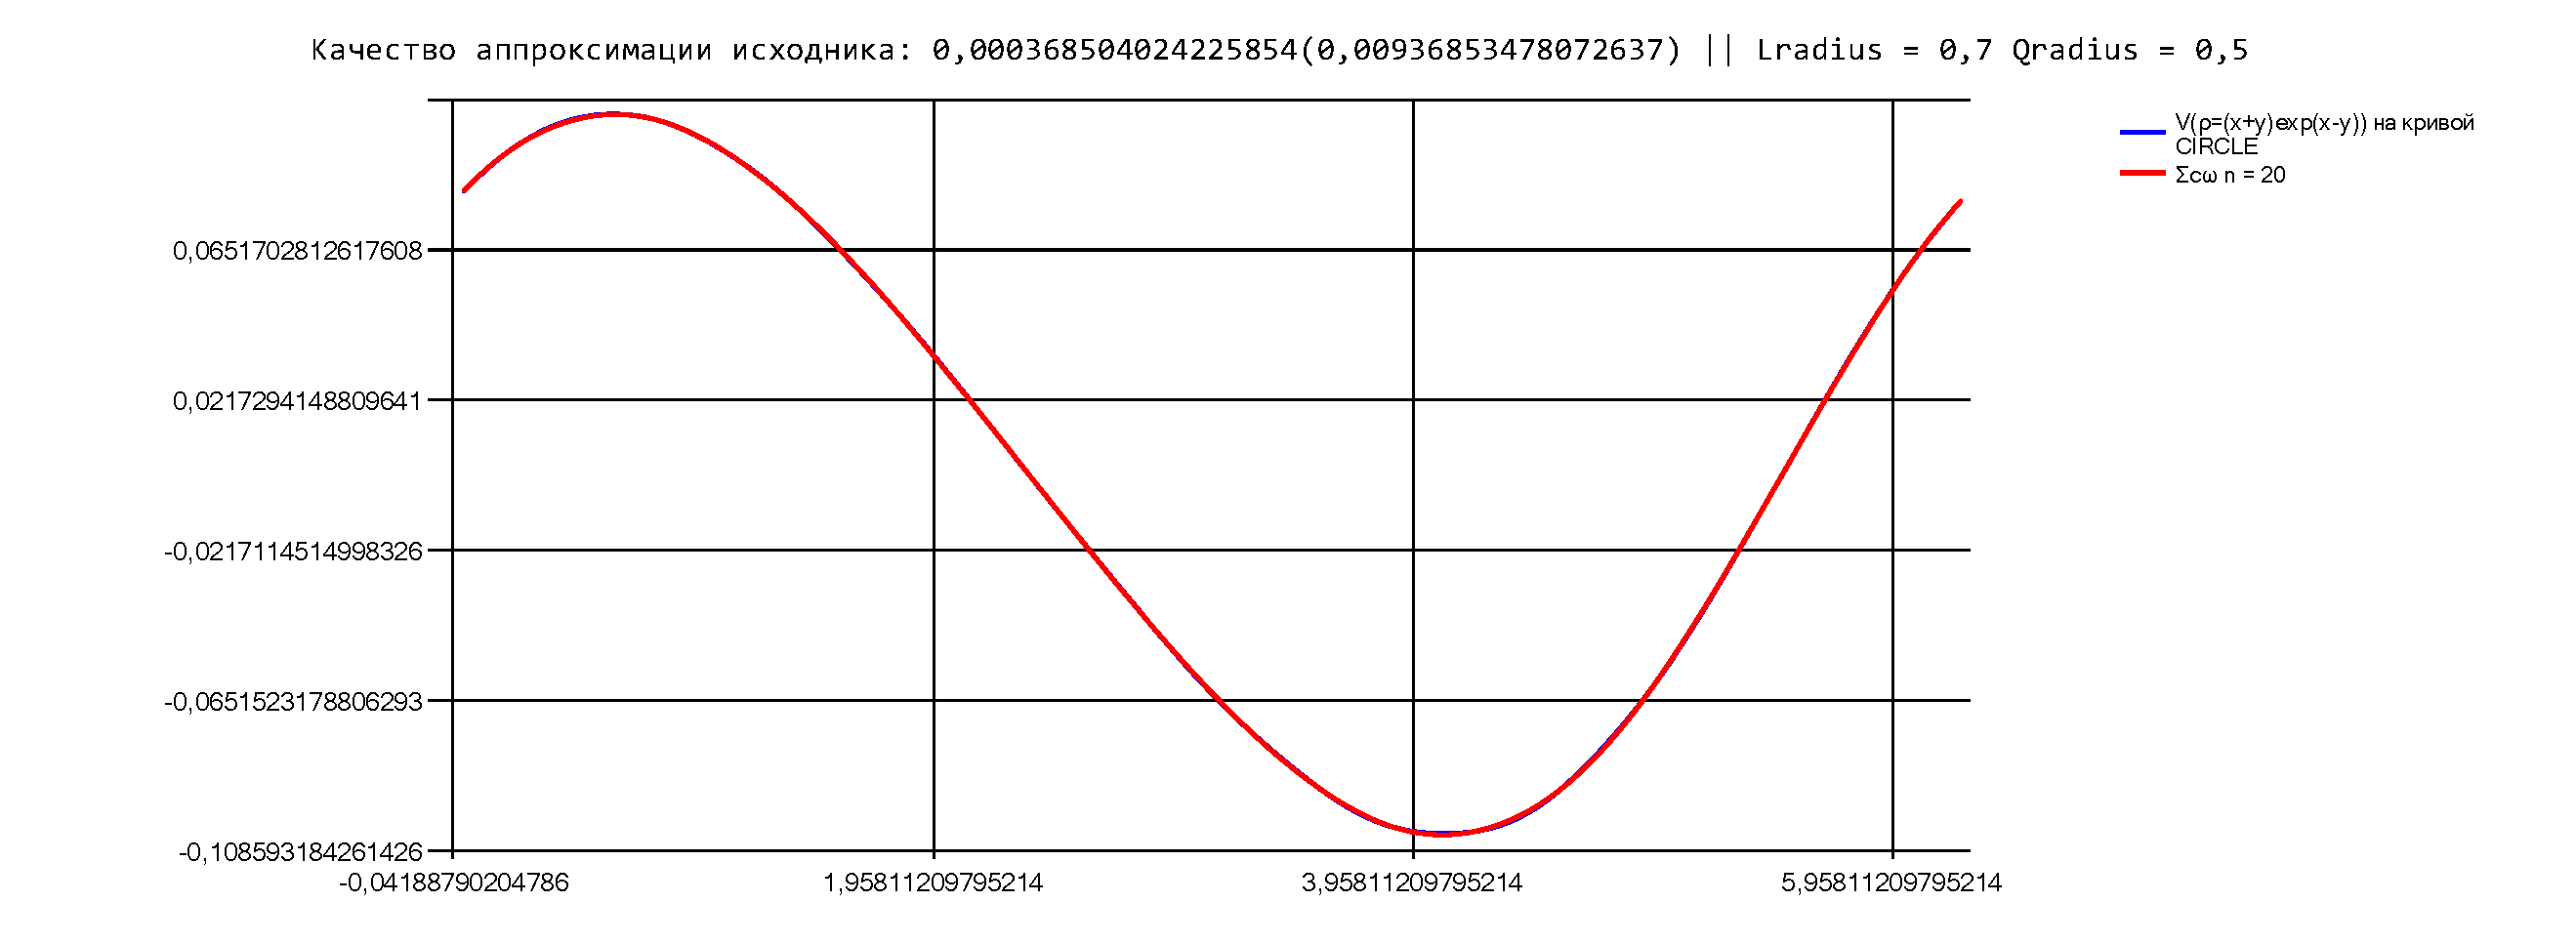
\includegraphics[width=0.8\linewidth]{v6.pdf} \\ для потенциала} 
            \end{minipage}} 
            \caption{Один из результатов работы метода} 
            \label{ris:image1} 
            \end{figure}

            \begin{figure}[h] 
              \center{\begin{minipage}[h]{\linewidth} 
              \center{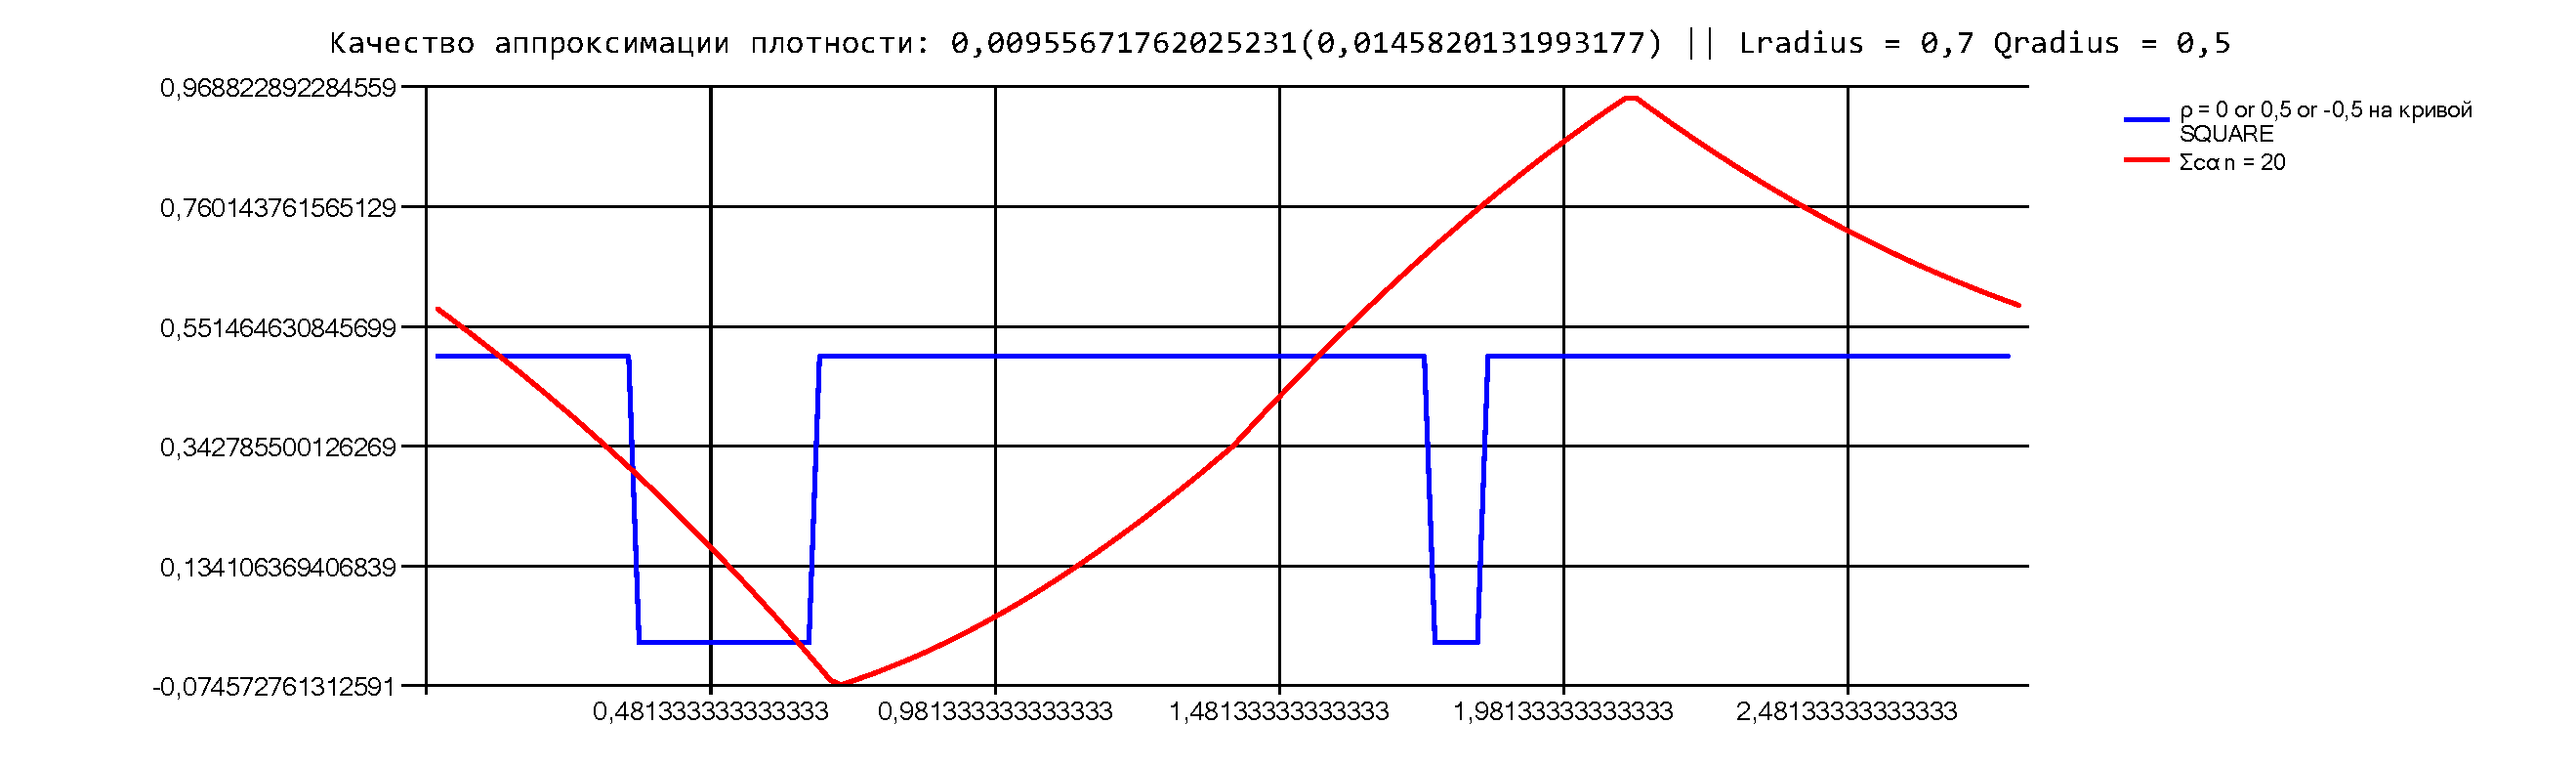
\includegraphics[width=0.8\linewidth]{d7.pdf} \\ для плотности} 
              \end{minipage}} 
              \vfill 
              \center{\begin{minipage}[h]{\linewidth} 
              \center{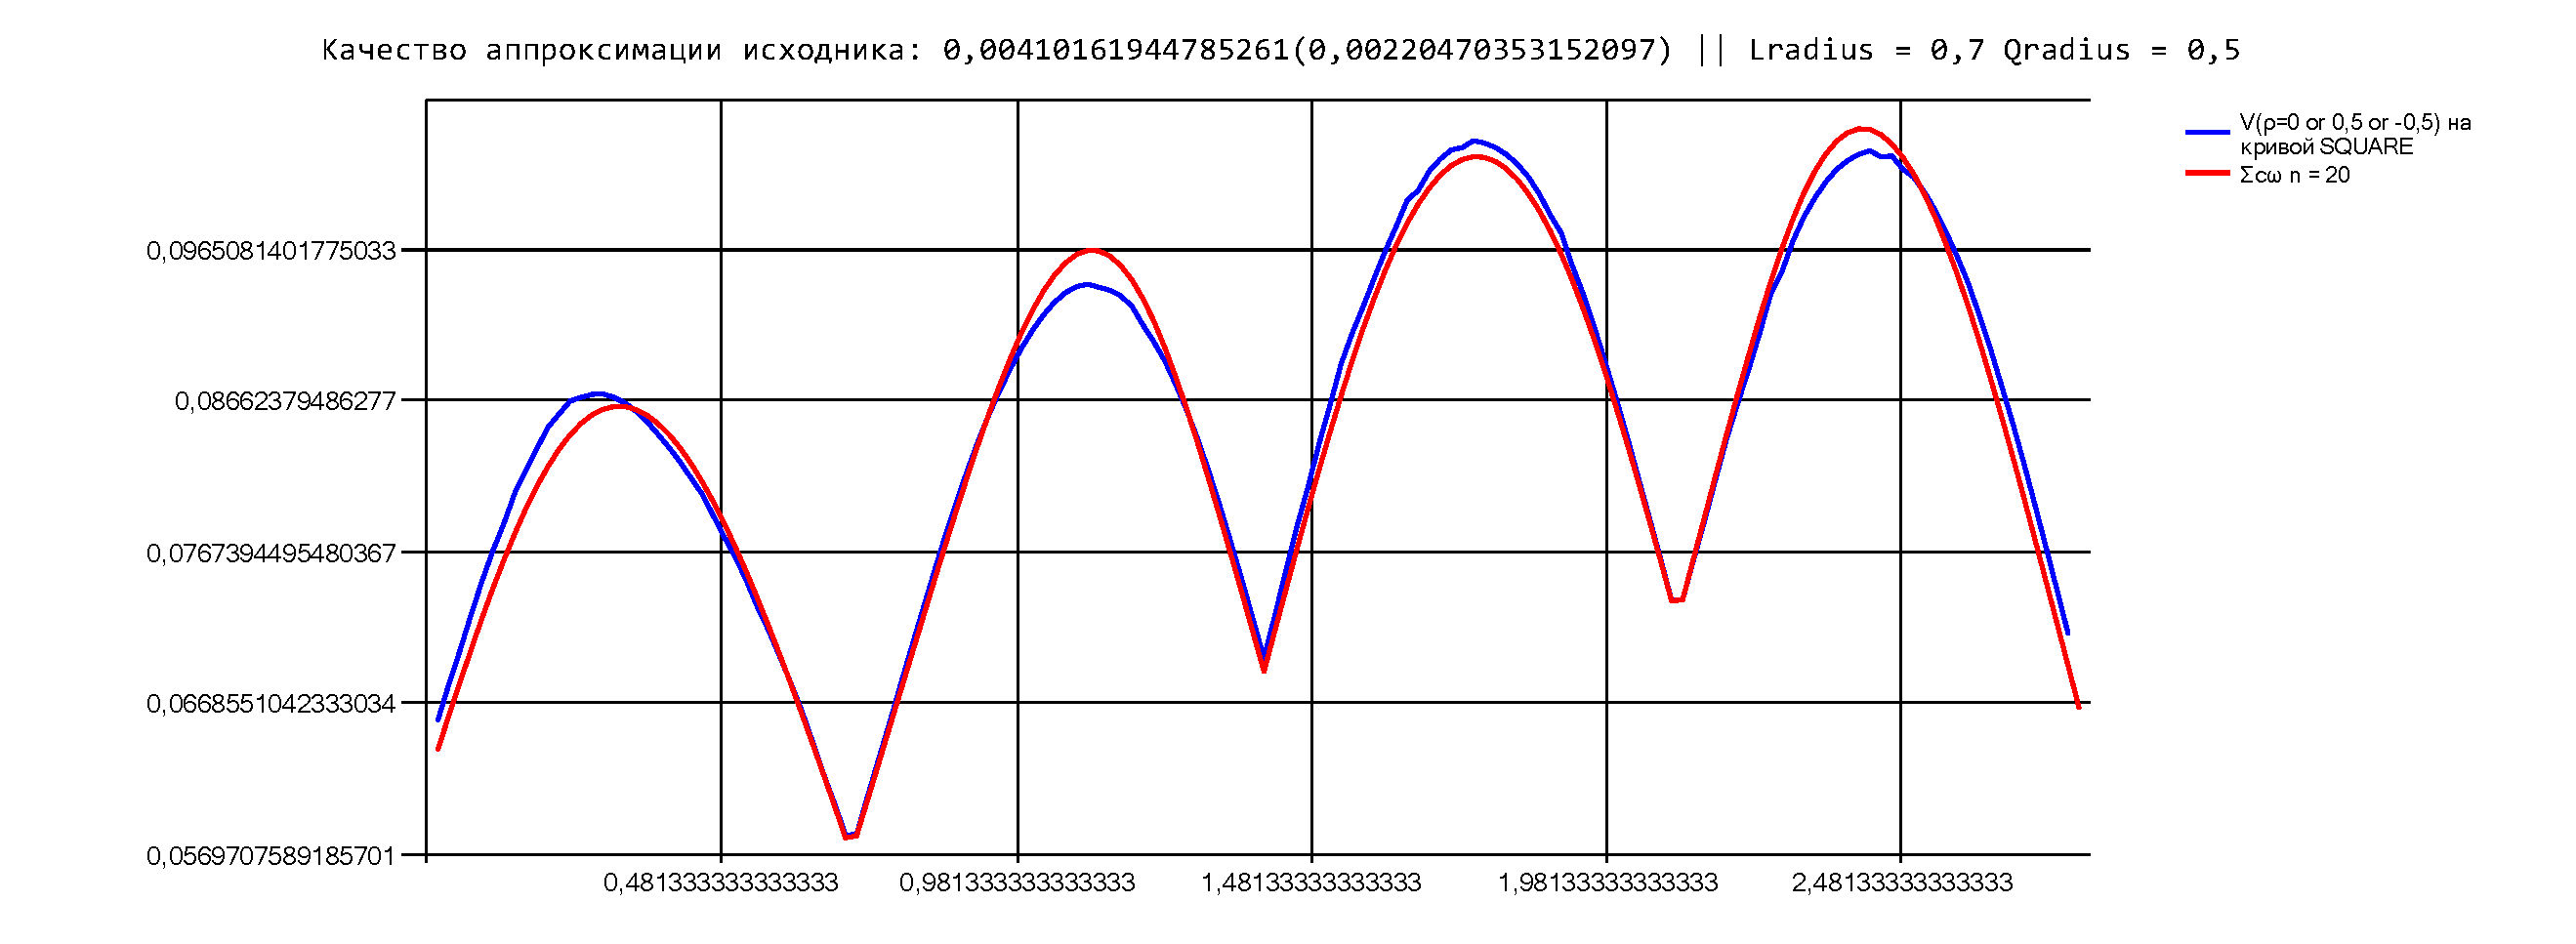
\includegraphics[width=0.8\linewidth]{v7.pdf} \\ для потенциала} 
              \end{minipage}} 
              \caption{Один из результатов работы метода} 
              \label{p1} 
              \end{figure}

              \begin{figure}[h] 
                \center{\begin{minipage}[h]{\linewidth} 
                \center{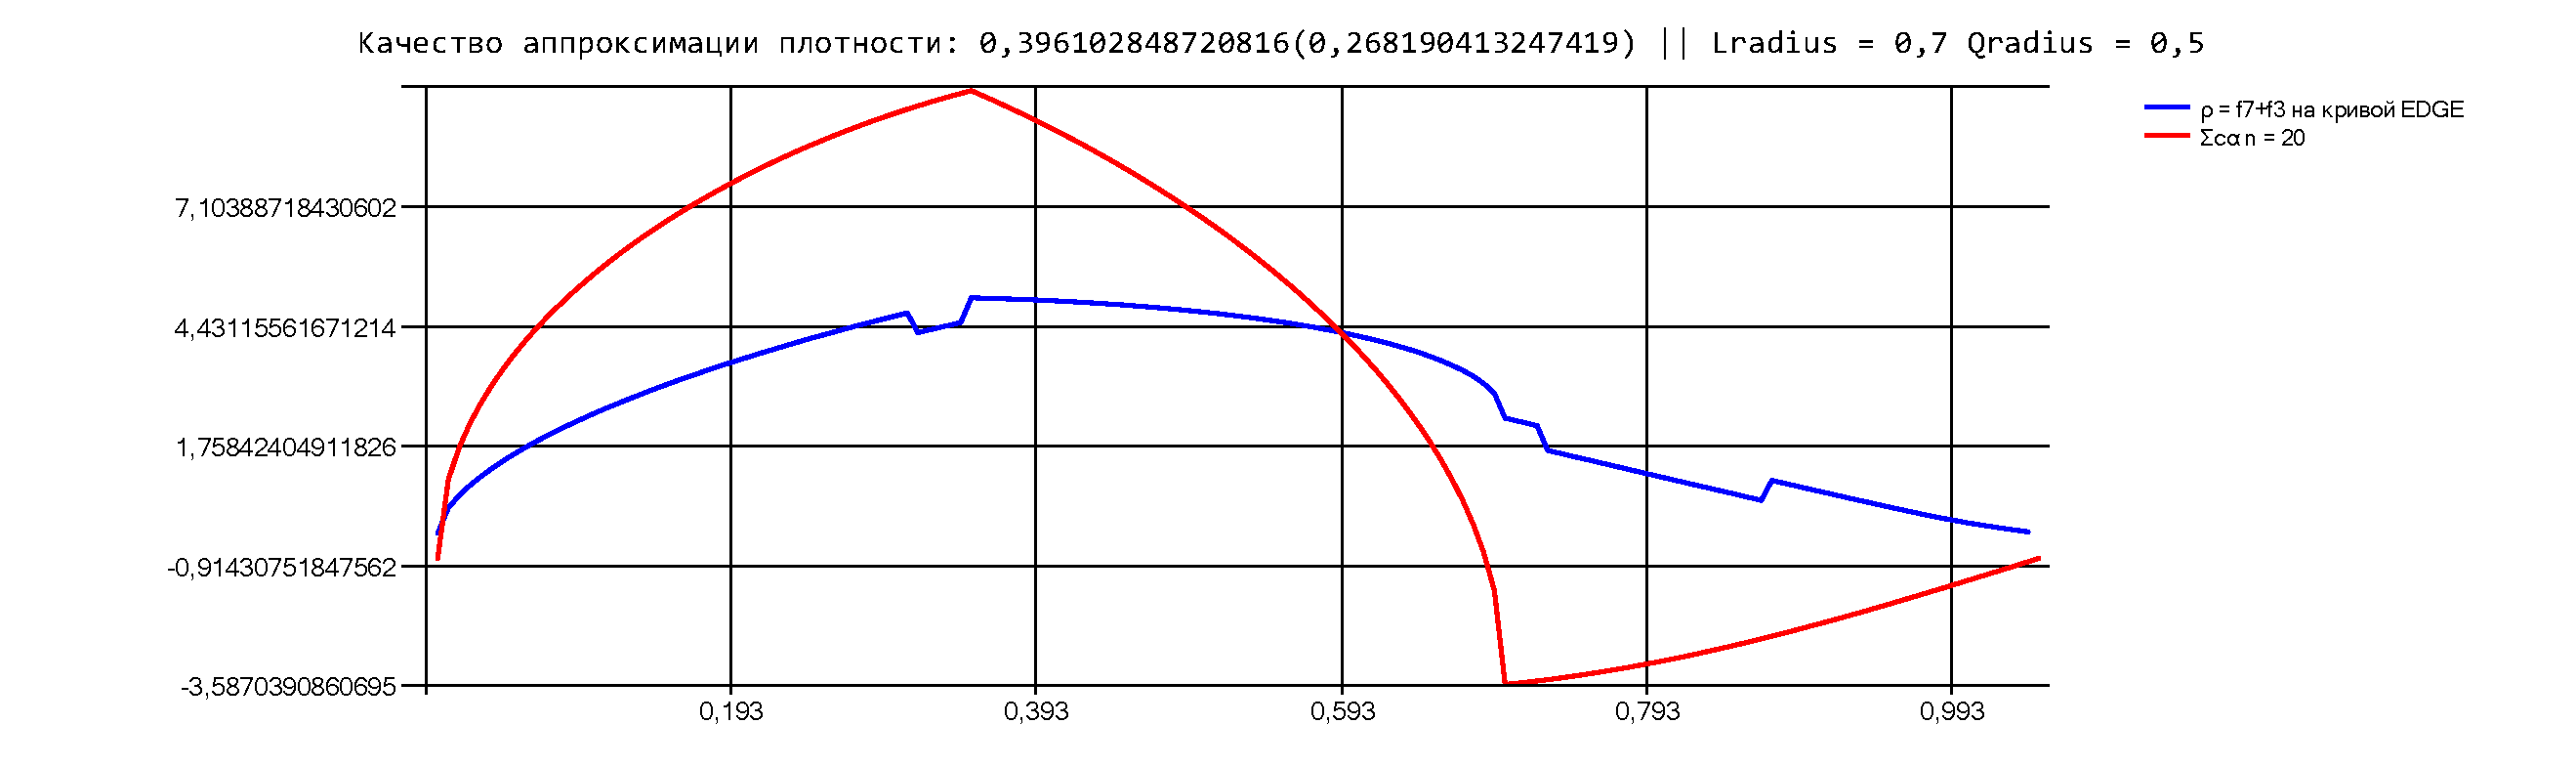
\includegraphics[width=0.8\linewidth]{d8.pdf} \\ для плотности} 
                \end{minipage}} 
                \vfill 
                \center{\begin{minipage}[h]{\linewidth} 
                \center{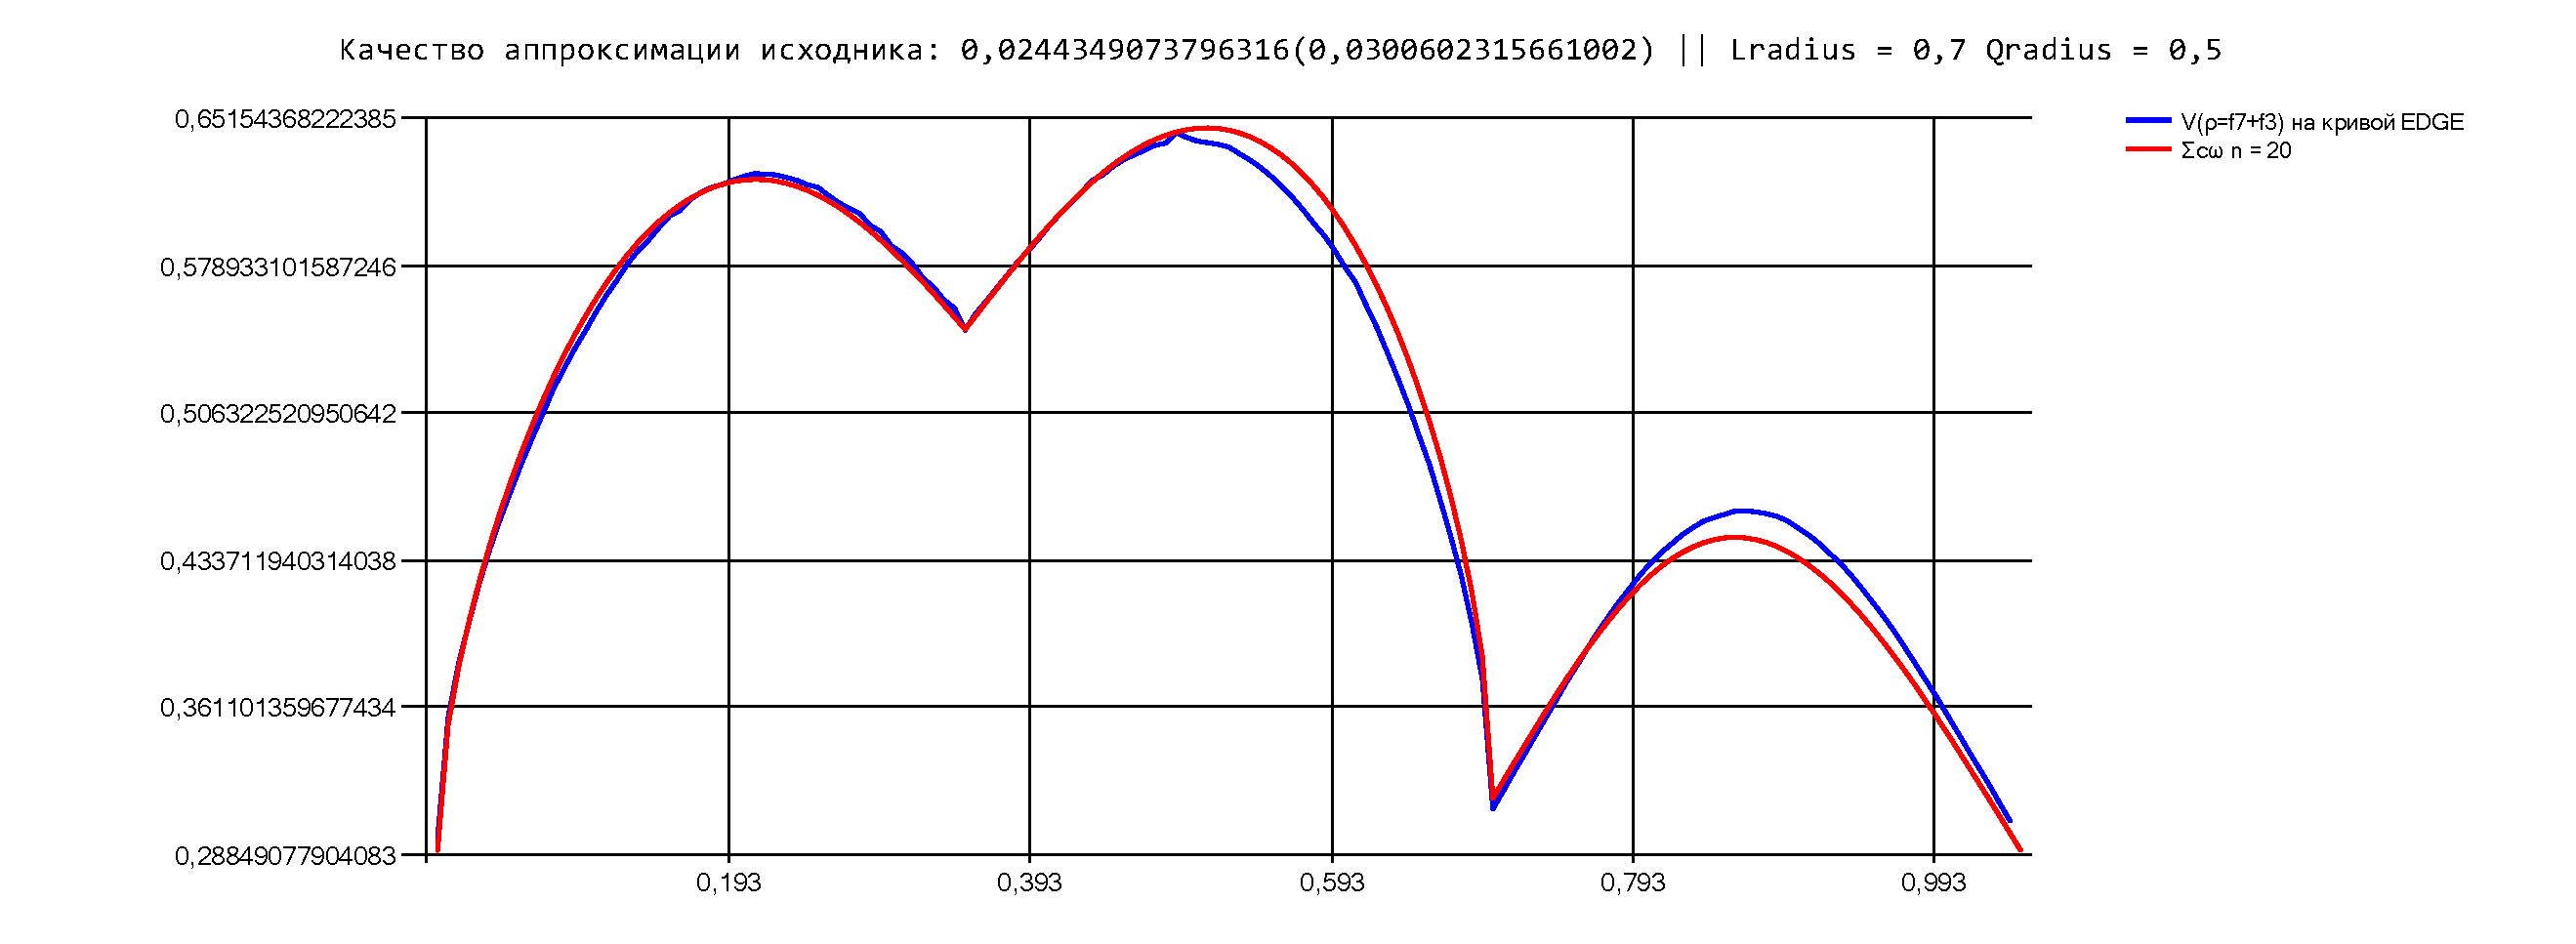
\includegraphics[width=0.8\linewidth]{v8.pdf} \\ для потенциала} 
                \end{minipage}} 
                \caption{Один из результатов работы метода} 
                \label{p2} 
                \end{figure}

                  \begin{figure}[h] 
                    \center{\begin{minipage}[h]{\linewidth} 
                    \center{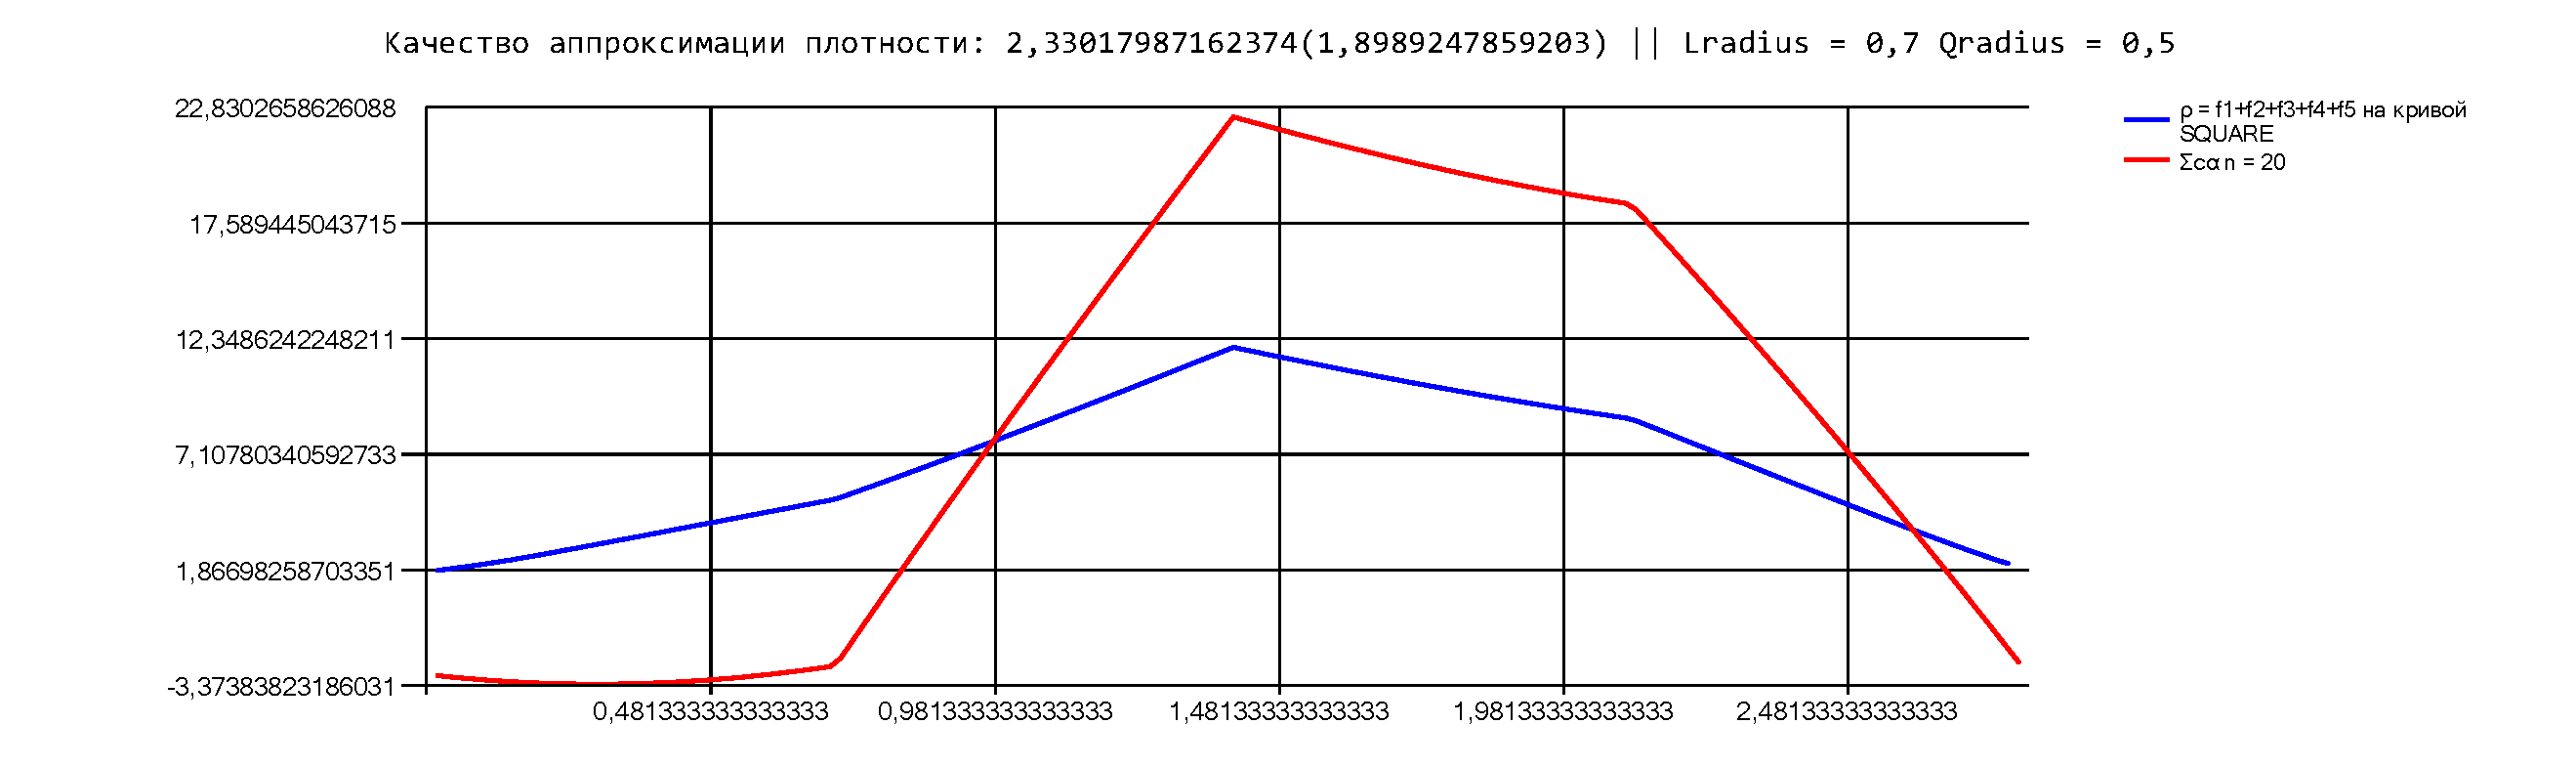
\includegraphics[width=0.8\linewidth]{d10.pdf} \\ для плотности} 
                    \end{minipage}} 
                    \vfill 
                    \center{\begin{minipage}[h]{\linewidth} 
                    \center{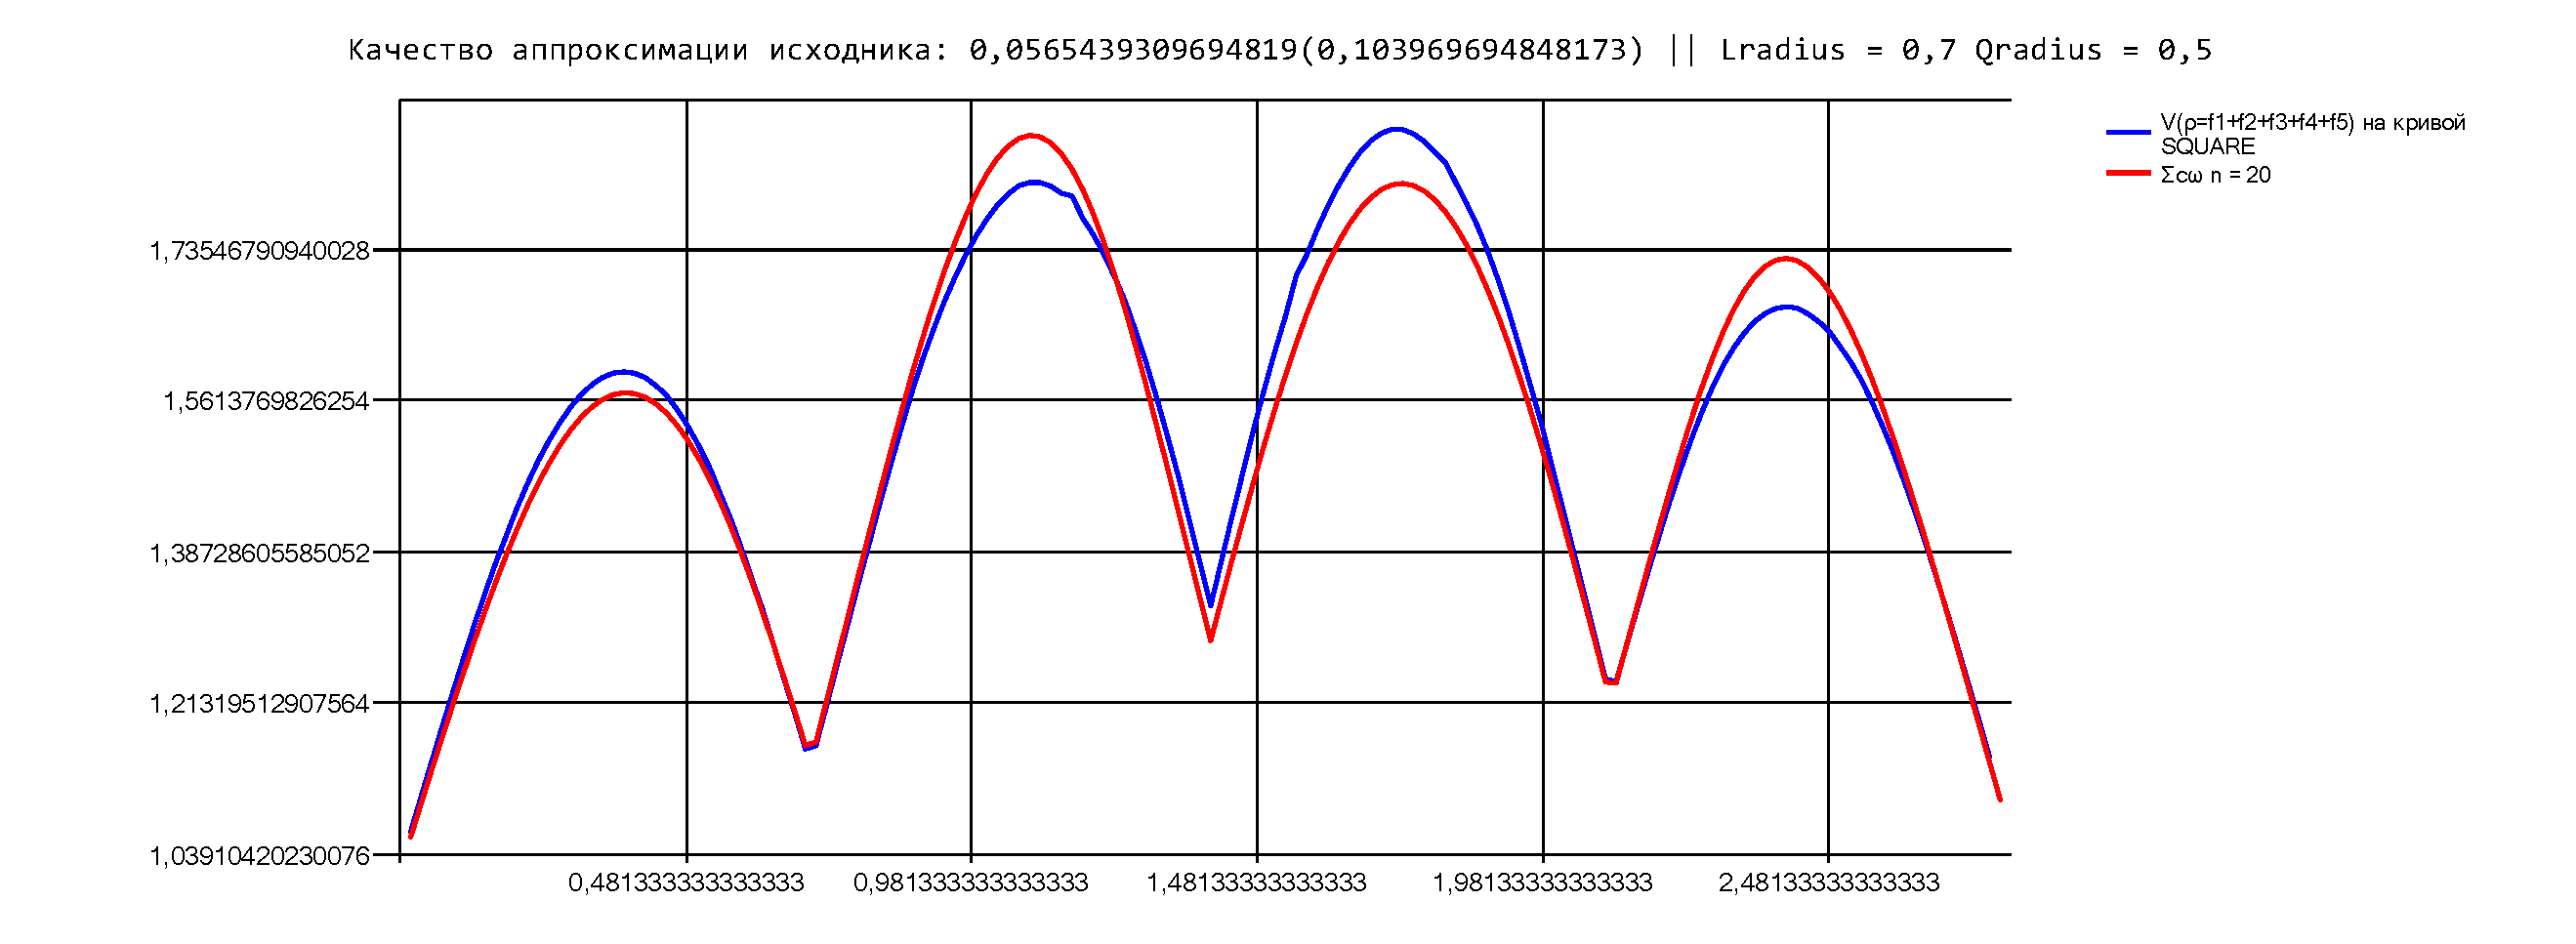
\includegraphics[width=0.8\linewidth]{v10.pdf} \\ для потенциала} 
                    \end{minipage}} 
                    \caption{Один из результатов работы метода} 
                    \label{hexampl} 
                    \end{figure}                                        

Рассмотрев результаты тестирования (около сотни графиков), я сделал вывод, что в среднем аппроксимация по круговой области происходит немного лучше.
%Для других областей, возможно, требует увеличивать точность интегрирования, либо сам характер области оказывает влияние на работу метода (на рисунке \ref{hexampl} показана аппроксимация первого базисного потенциала на треугольнике, которая логически должна составлял абсолютный ноль).
Однако, некоторые функции лучше аппроксимировались на некруговых областях.
Кроме этого, хорошая аппроксимация $||V_f-V_{\tilde{\rho} } ||_{L_2(L)}$ не всегда означает хорошую аппроксимацию $||\rho-\tilde{\rho} ||_{L_2(Q)}$ (неустойчивость заметна на многих рисунках).%, рисунки \ref{p1},\ref{p2},\ref{p3},\ref{p4},\ref{p5},\ref{p6},\ref{p7}).

\FloatBarrier 
\subsubsection{3D-графики}
Если 2D-графики из прошлого подраздела показывали особенности аппроксимации на границе области $Q$, то следующие графики показывают поведение погрешности по всей области в целом.
В графиках (рисунки \ref{d3beg}-\ref{d3end}) число базисных потенциалов равно $20$, под Density имеется в виду плотность $\rho$, под Density approx. --- $\tilde{\rho}$, под Difference --- функция $|\rho-\tilde{\rho}|$.

\begin{figure}[h]
  \begin{minipage}[h]{0.49\linewidth}
  \center{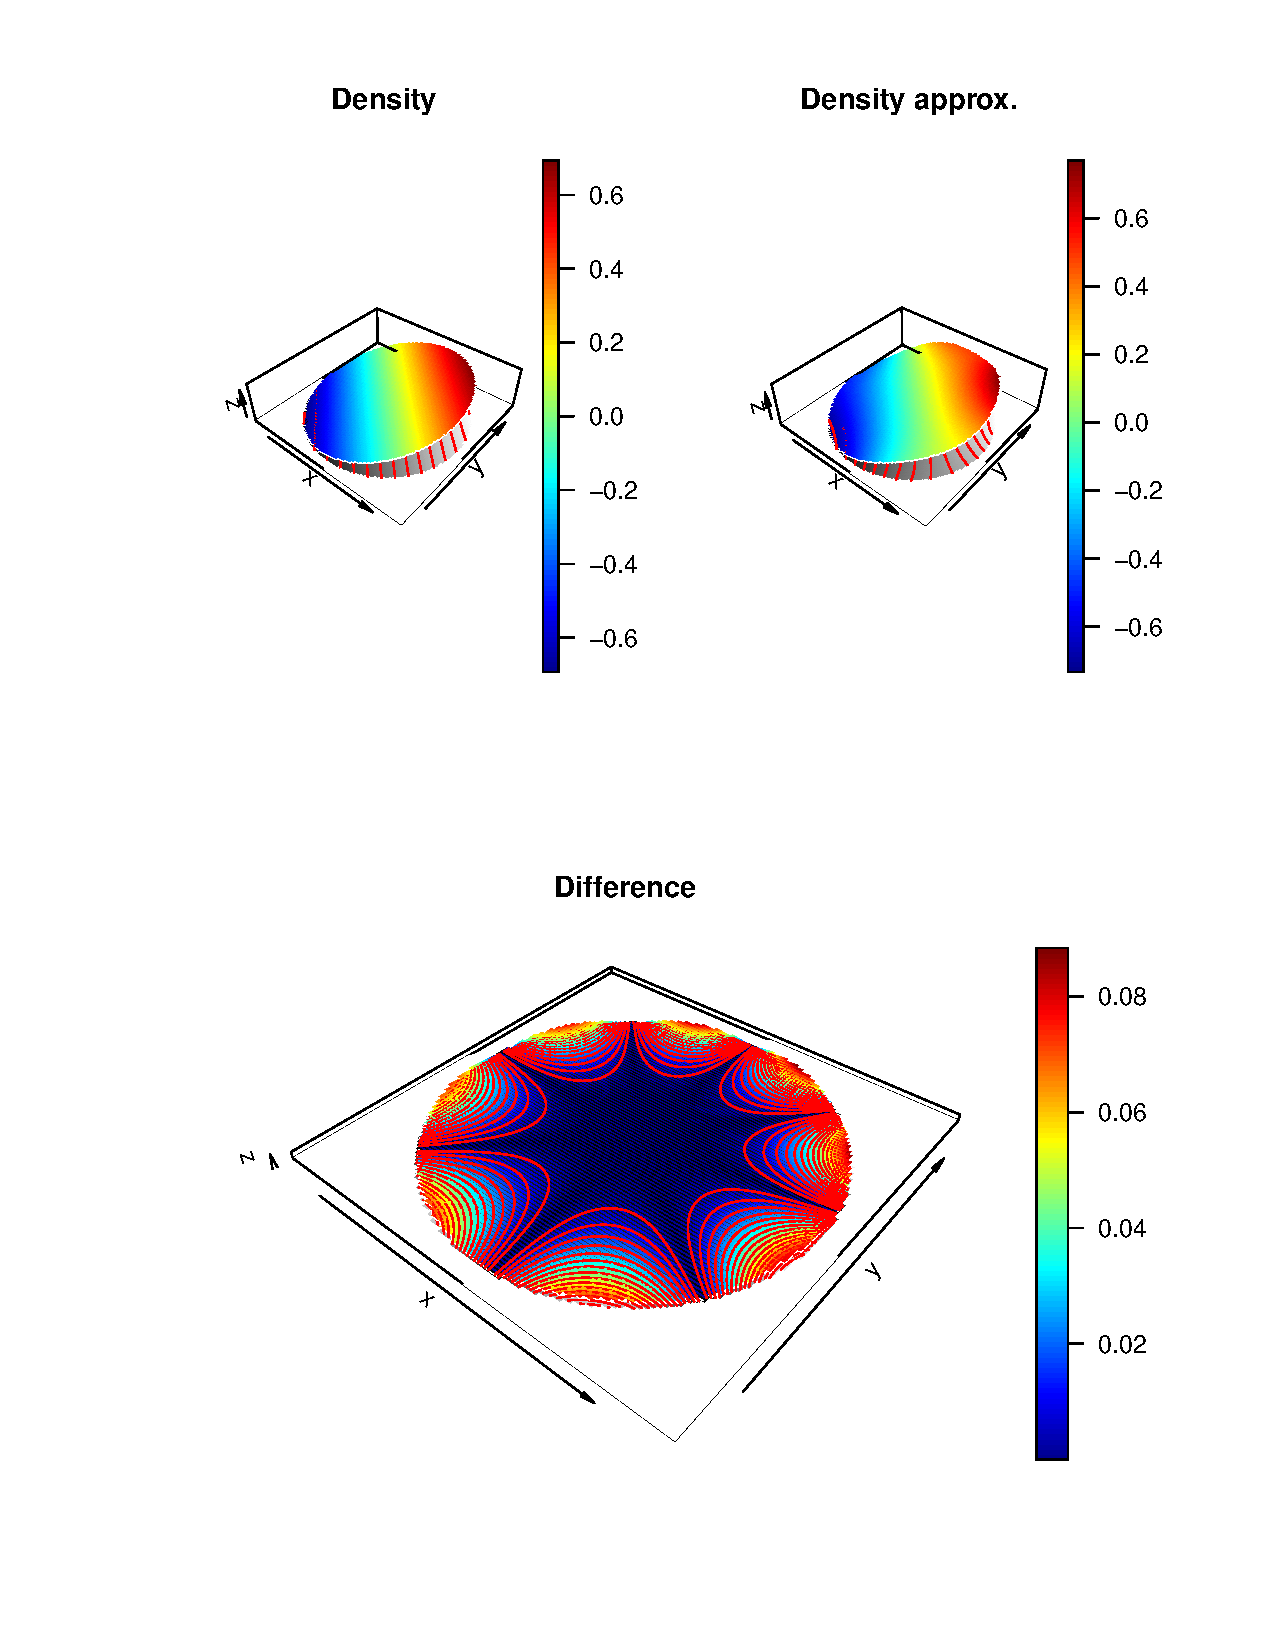
\includegraphics[width=0.95\linewidth]{f11.pdf}}
  \end{minipage}
  \hfill
  \begin{minipage}[h]{0.49\linewidth}
  \center{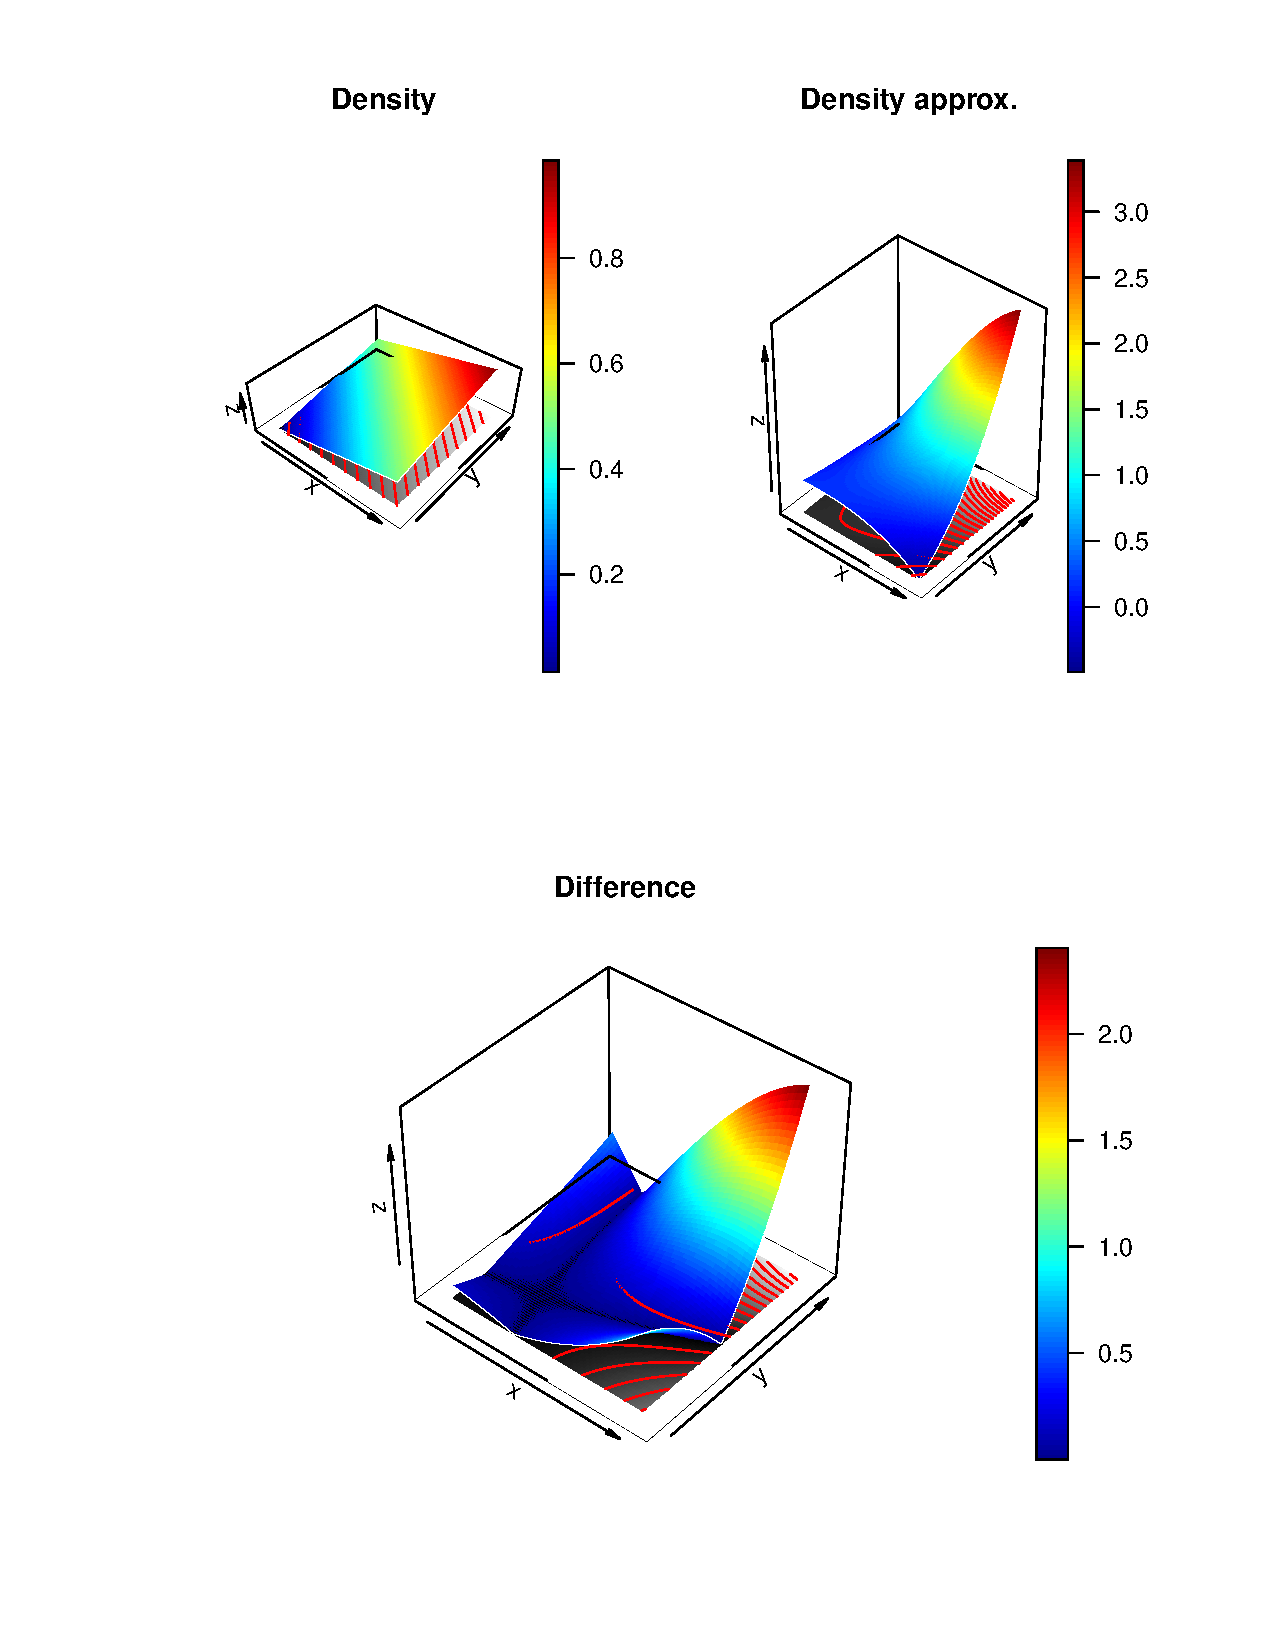
\includegraphics[width=0.95\linewidth]{f13.pdf}}
  \end{minipage}
  \caption{Для $f_1$}
  \label{d3beg}
  \end{figure}

  \begin{figure}[h]
    \begin{minipage}[h]{0.49\linewidth}
    \center{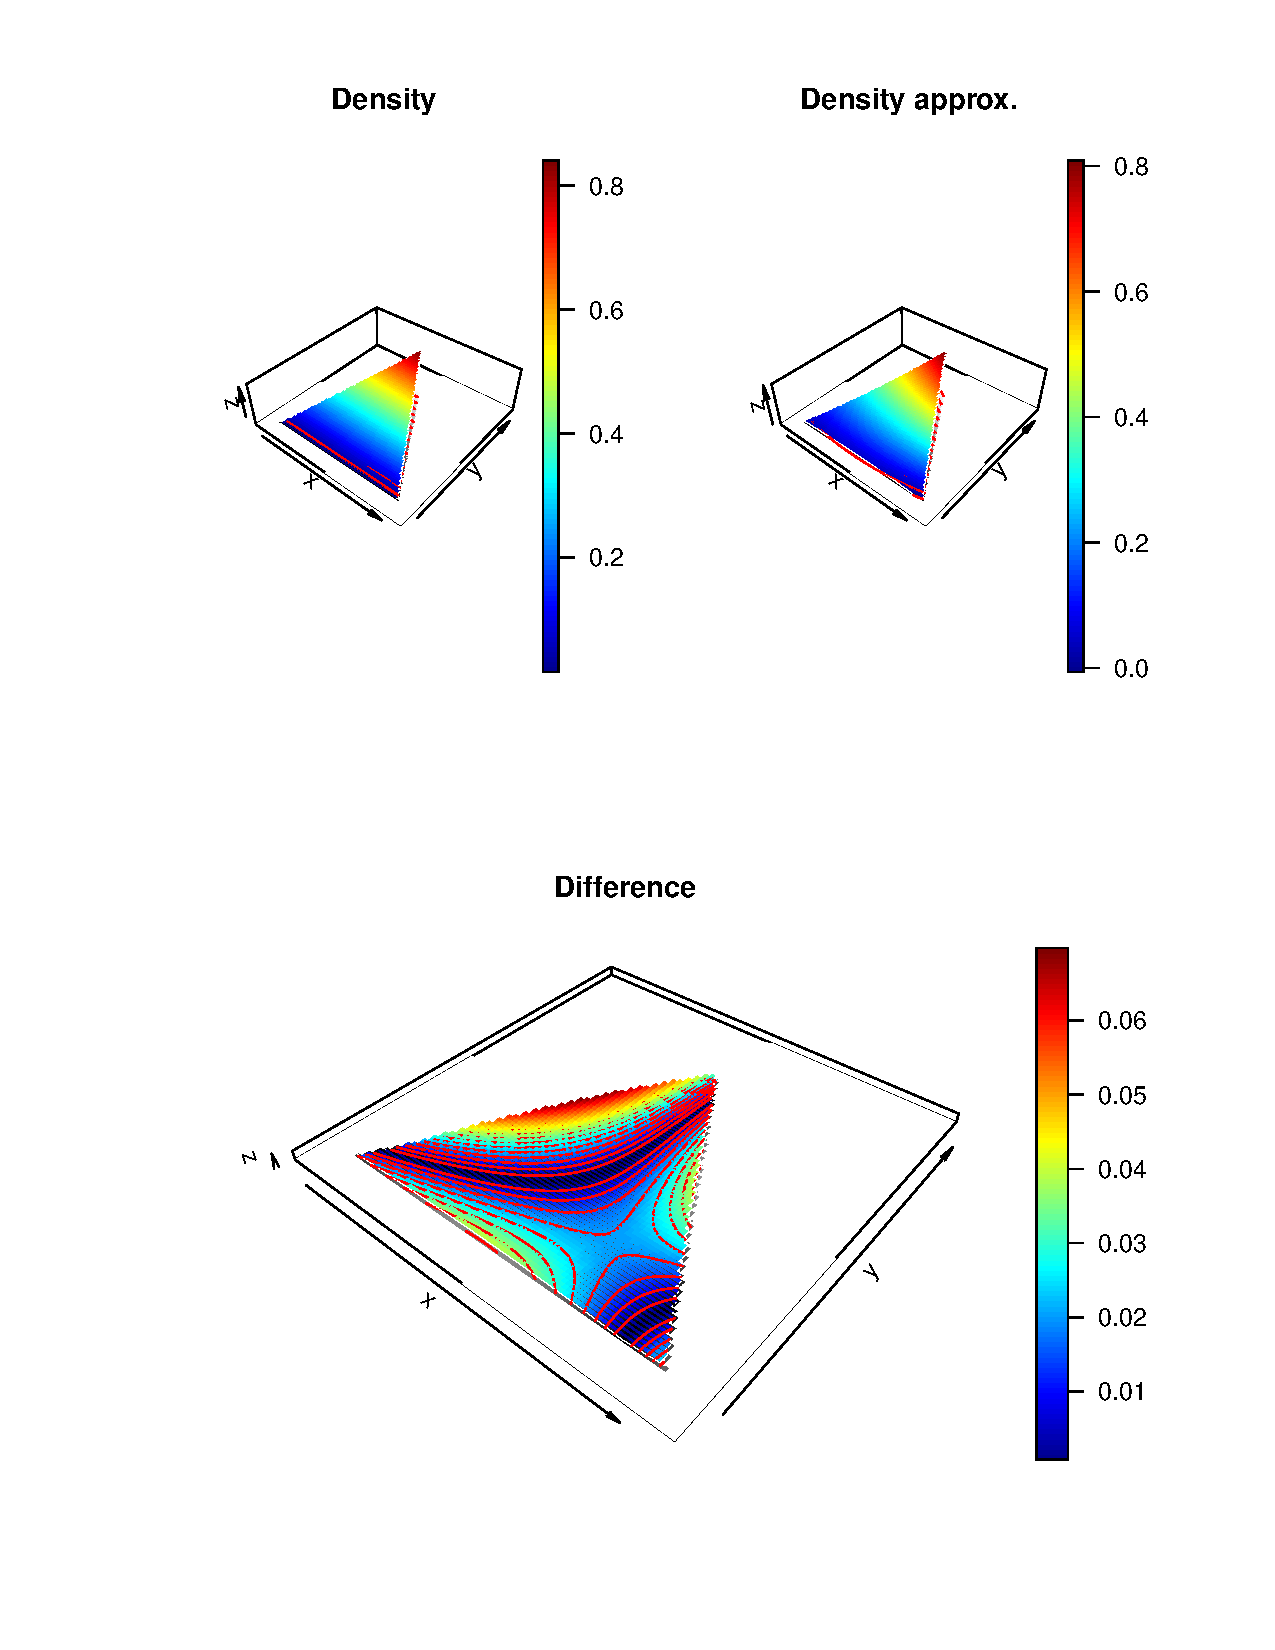
\includegraphics[width=0.95\linewidth]{f22.pdf}}
    \end{minipage}
    \hfill
    \begin{minipage}[h]{0.49\linewidth}
    \center{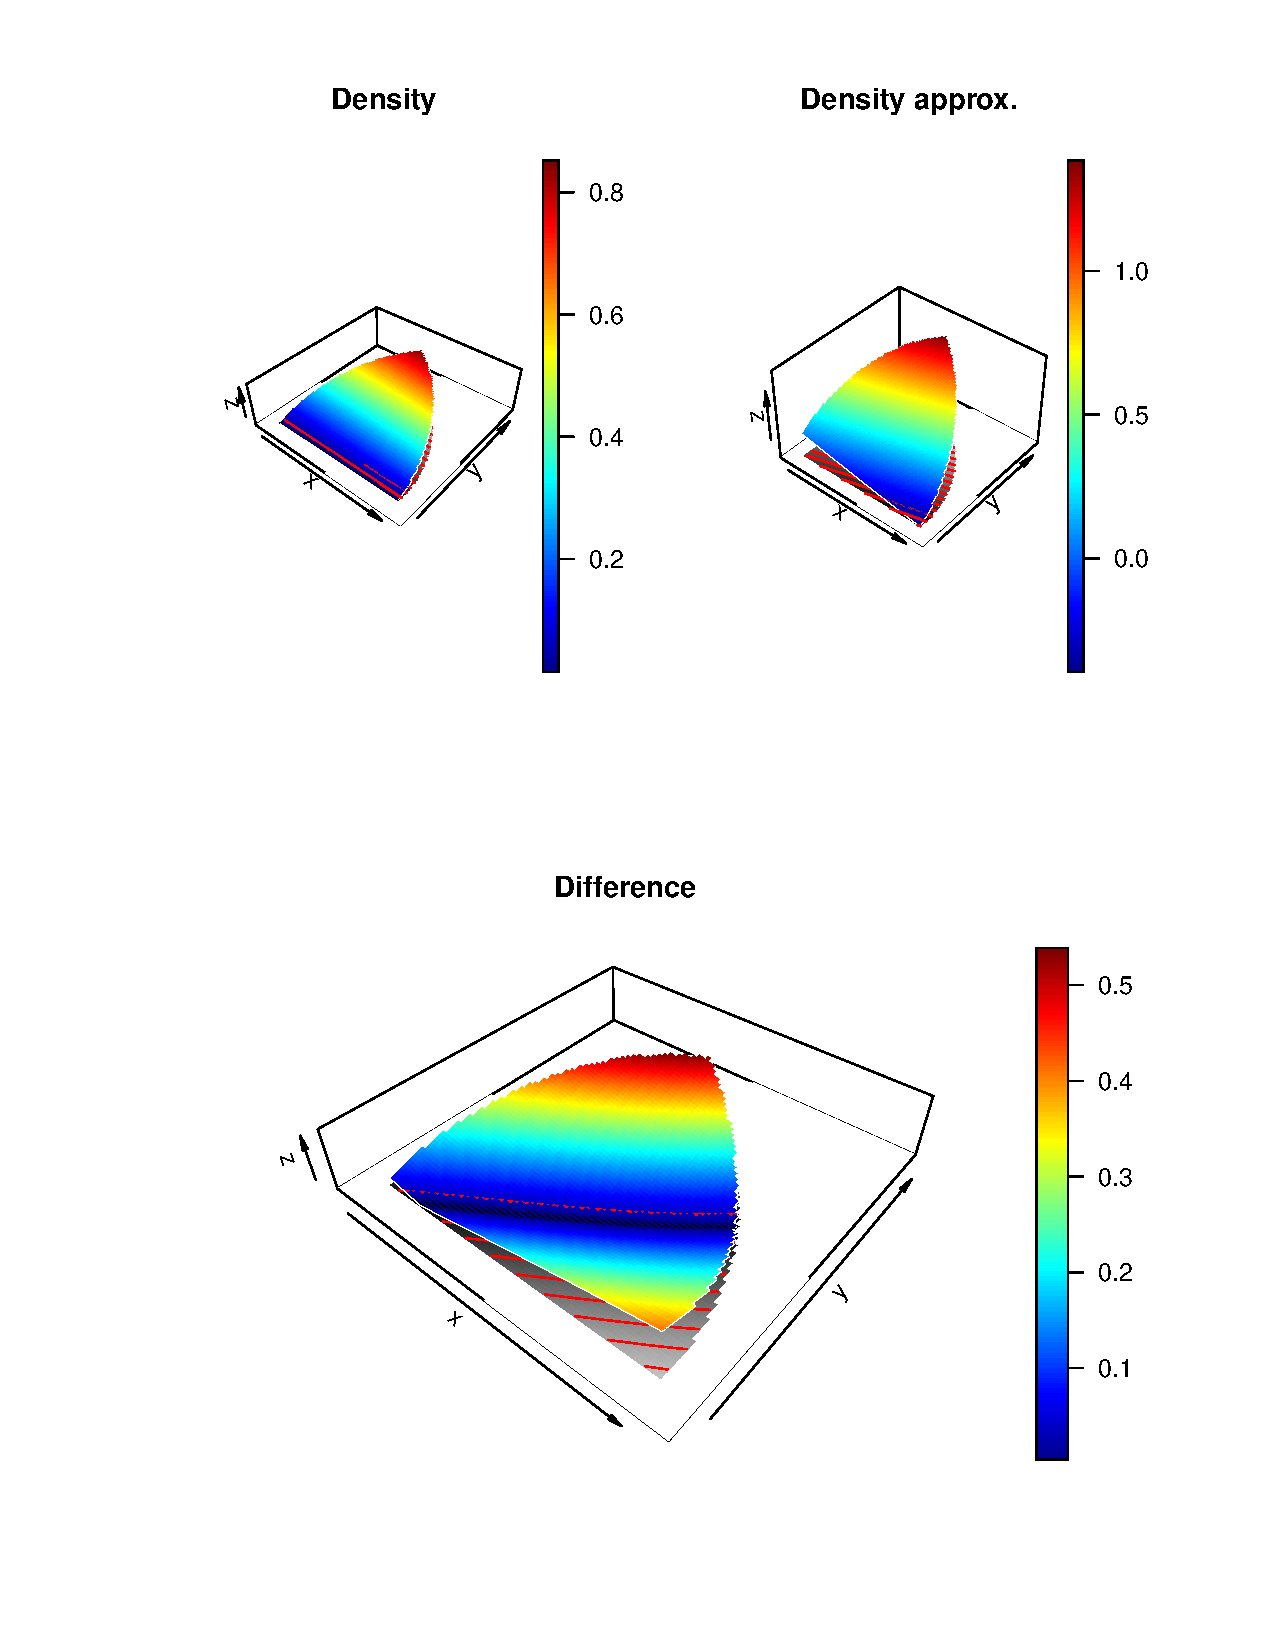
\includegraphics[width=0.95\linewidth]{f24.pdf}}
    \end{minipage}
    \caption{Для $f_2$}
    \label{ris:image1}
    \end{figure}

    \begin{figure}[h]
      \begin{minipage}[h]{0.49\linewidth}
      \center{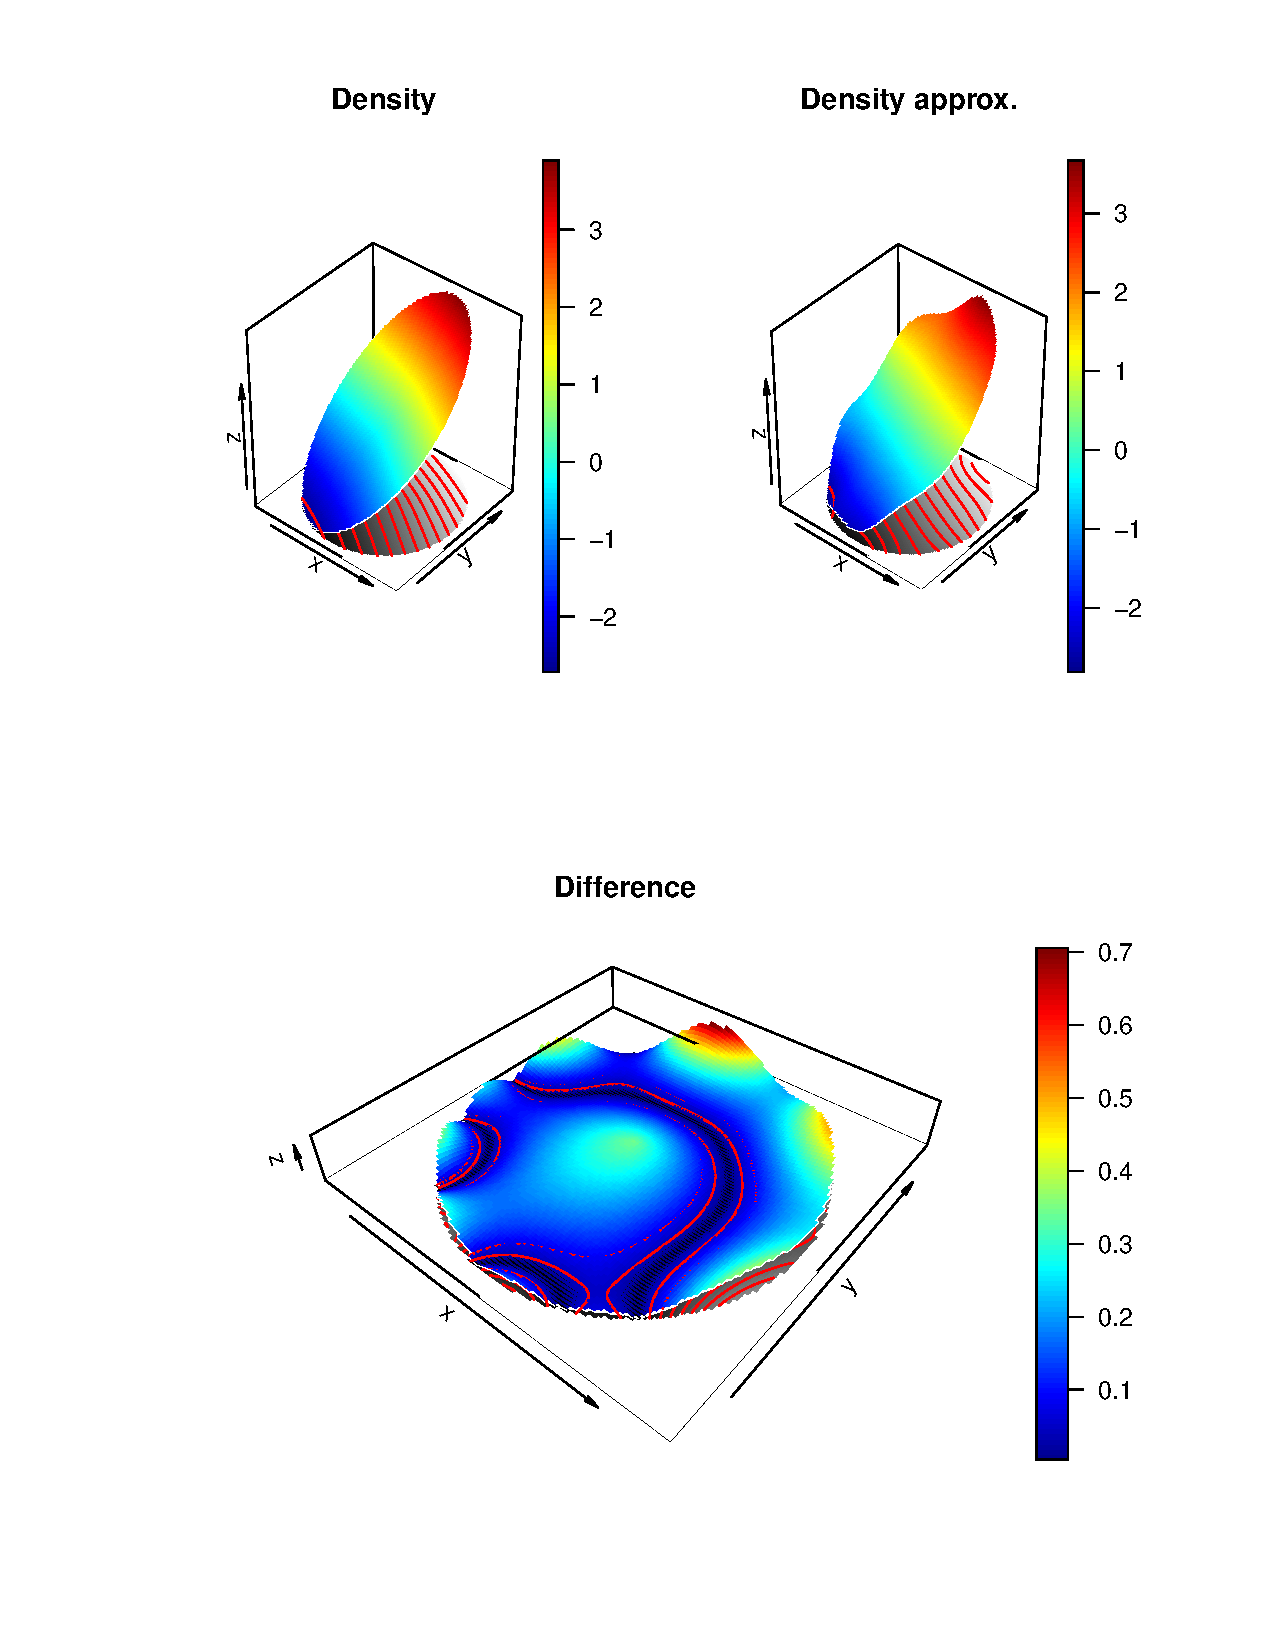
\includegraphics[width=0.95\linewidth]{f31.pdf}}
      \end{minipage}
      \hfill
      \begin{minipage}[h]{0.49\linewidth}
      \center{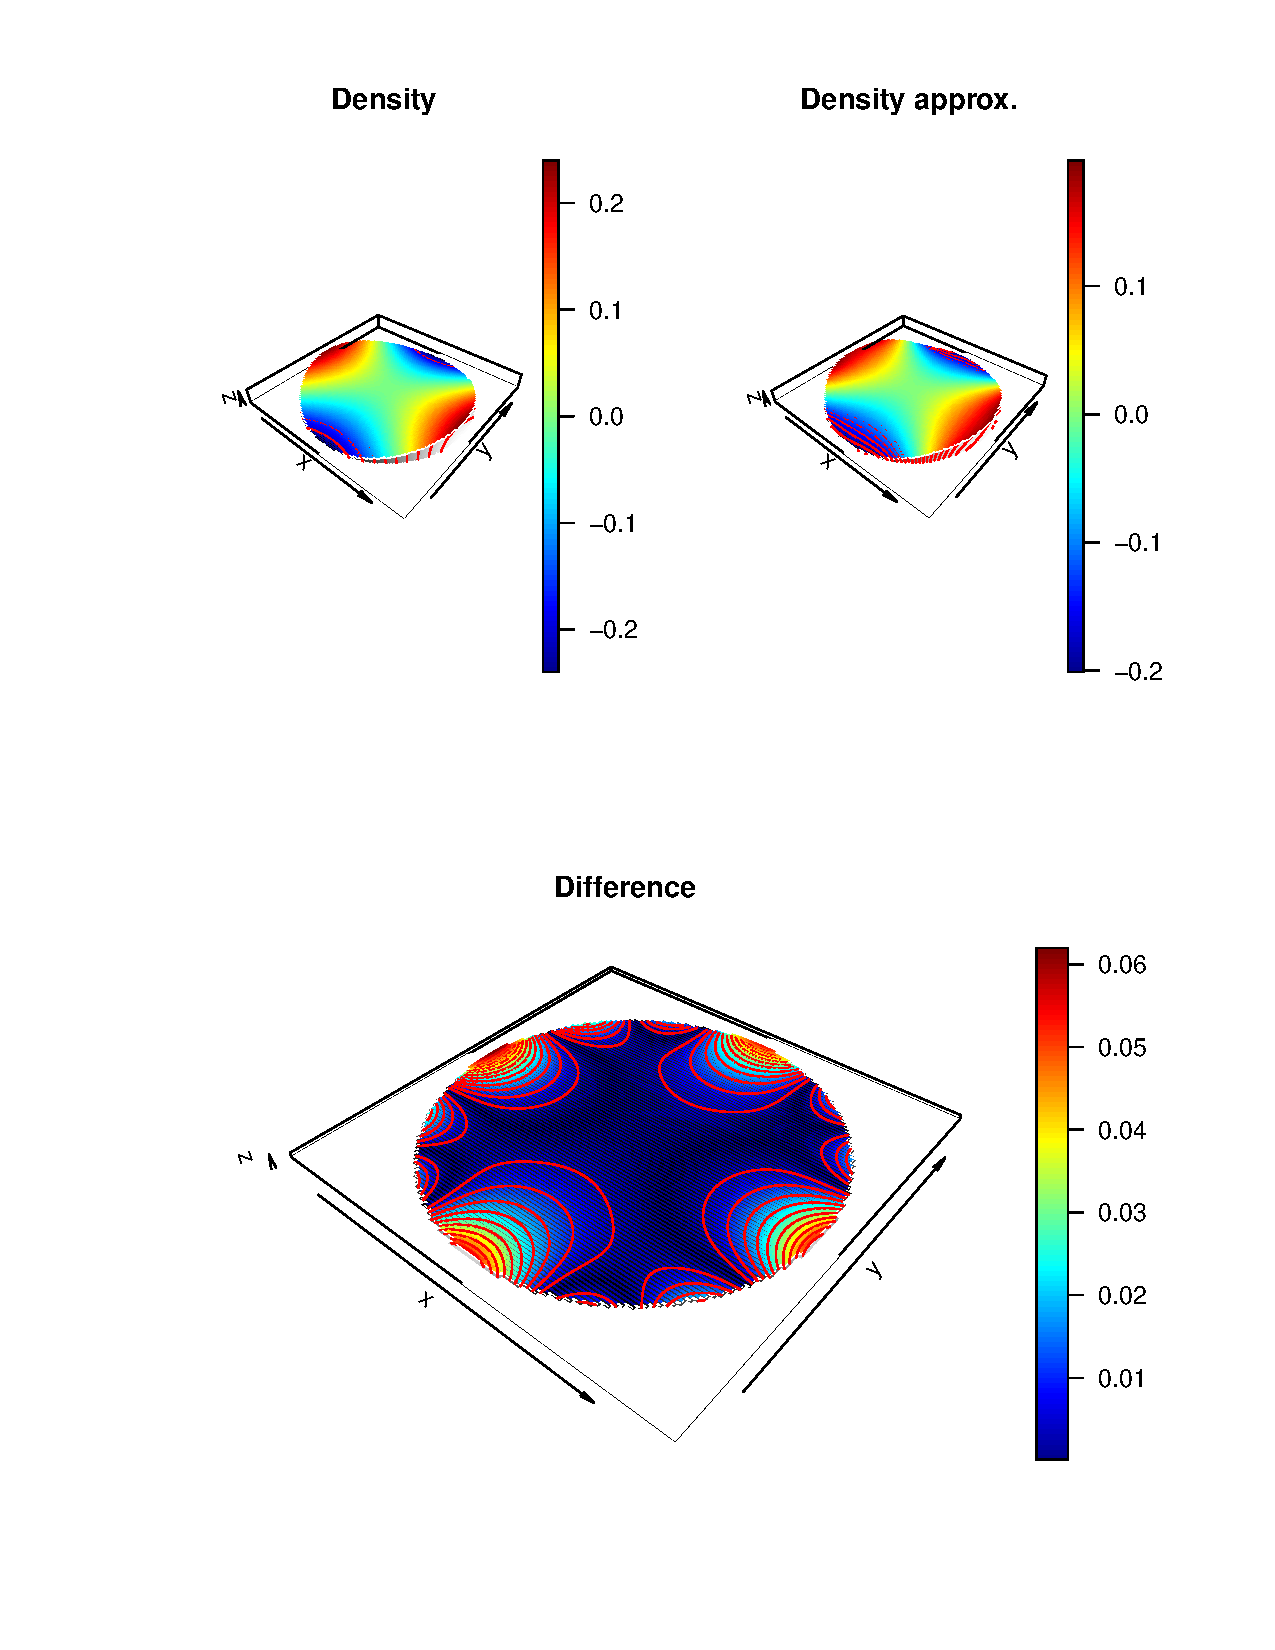
\includegraphics[width=0.95\linewidth]{f51.pdf}}
      \end{minipage}
      \caption{Для $f_3$ и $f_5$}
      \label{ris:image1}
      \end{figure}

    \begin{figure}[h]
      \begin{minipage}[h]{0.49\linewidth}
      \center{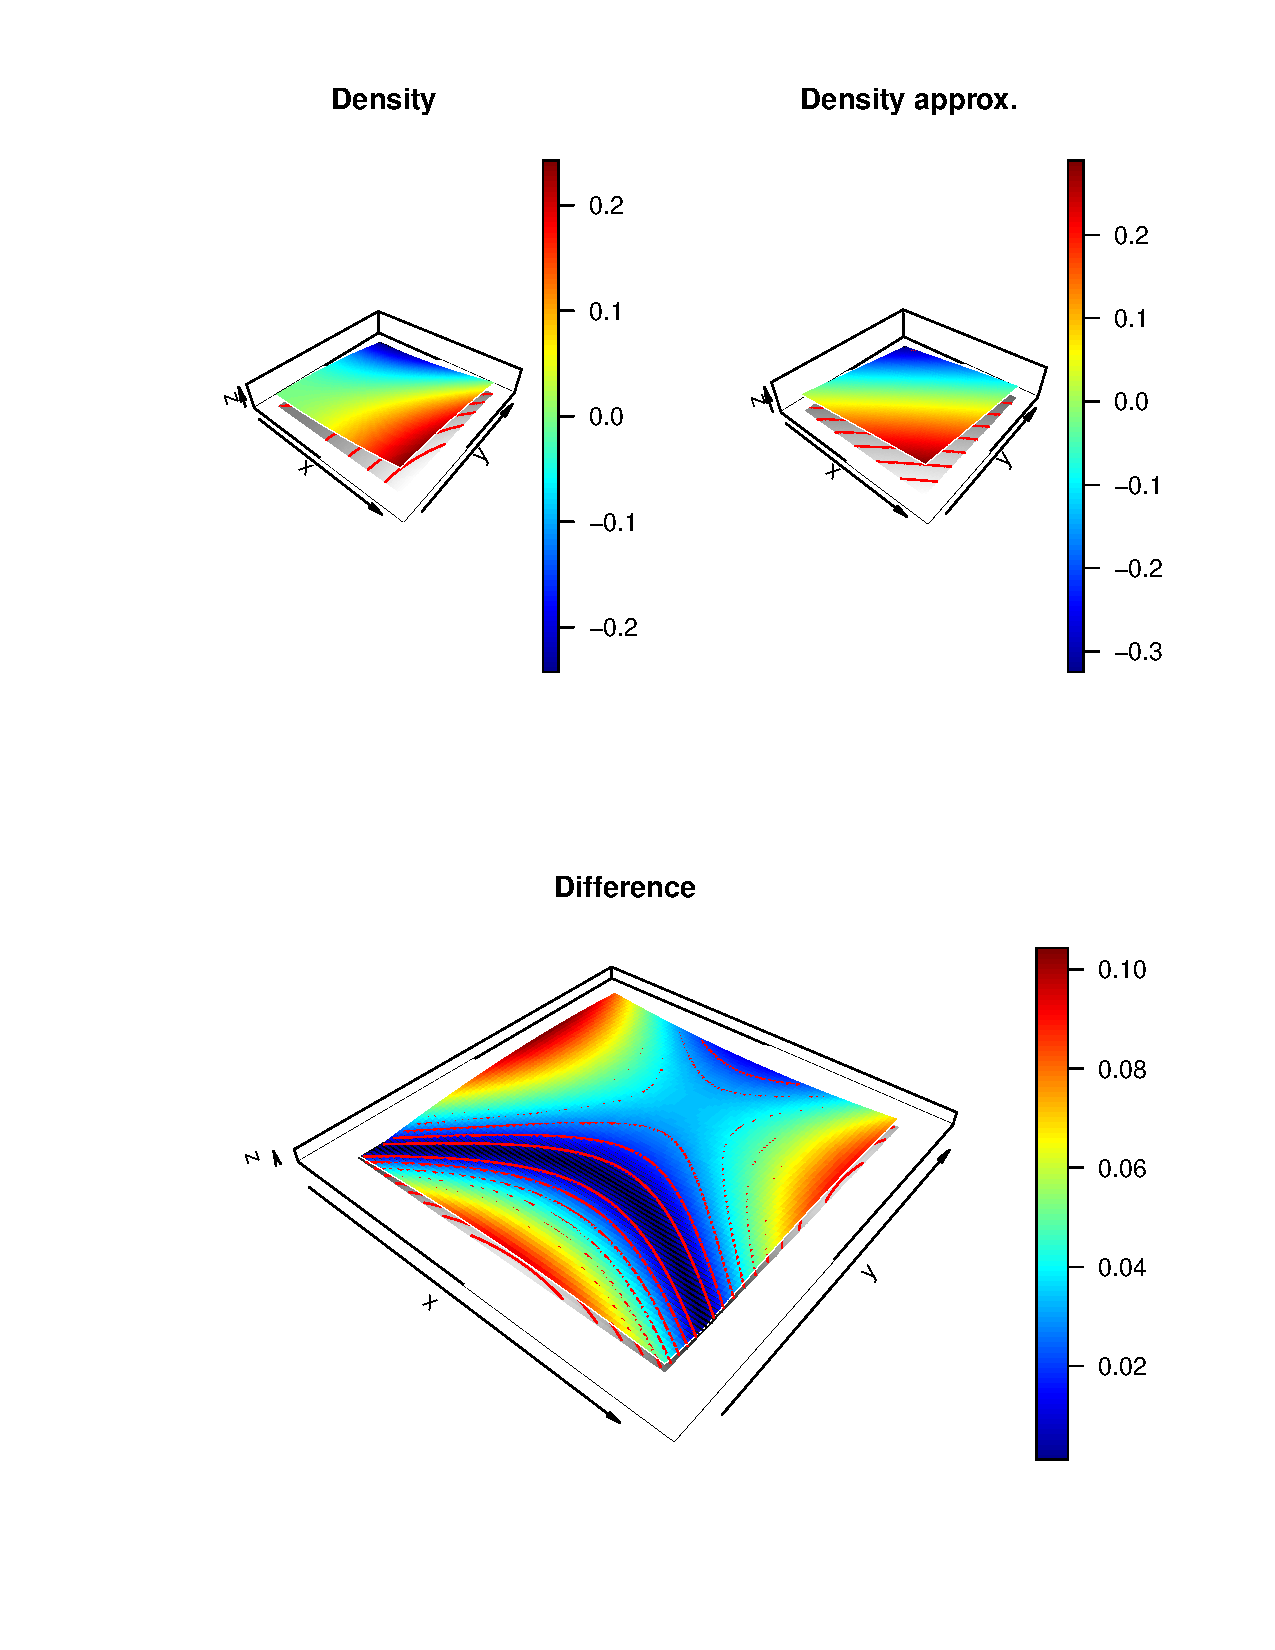
\includegraphics[width=0.95\linewidth]{f53.pdf}}
      \end{minipage}
      \hfill
      \begin{minipage}[h]{0.49\linewidth}
      \center{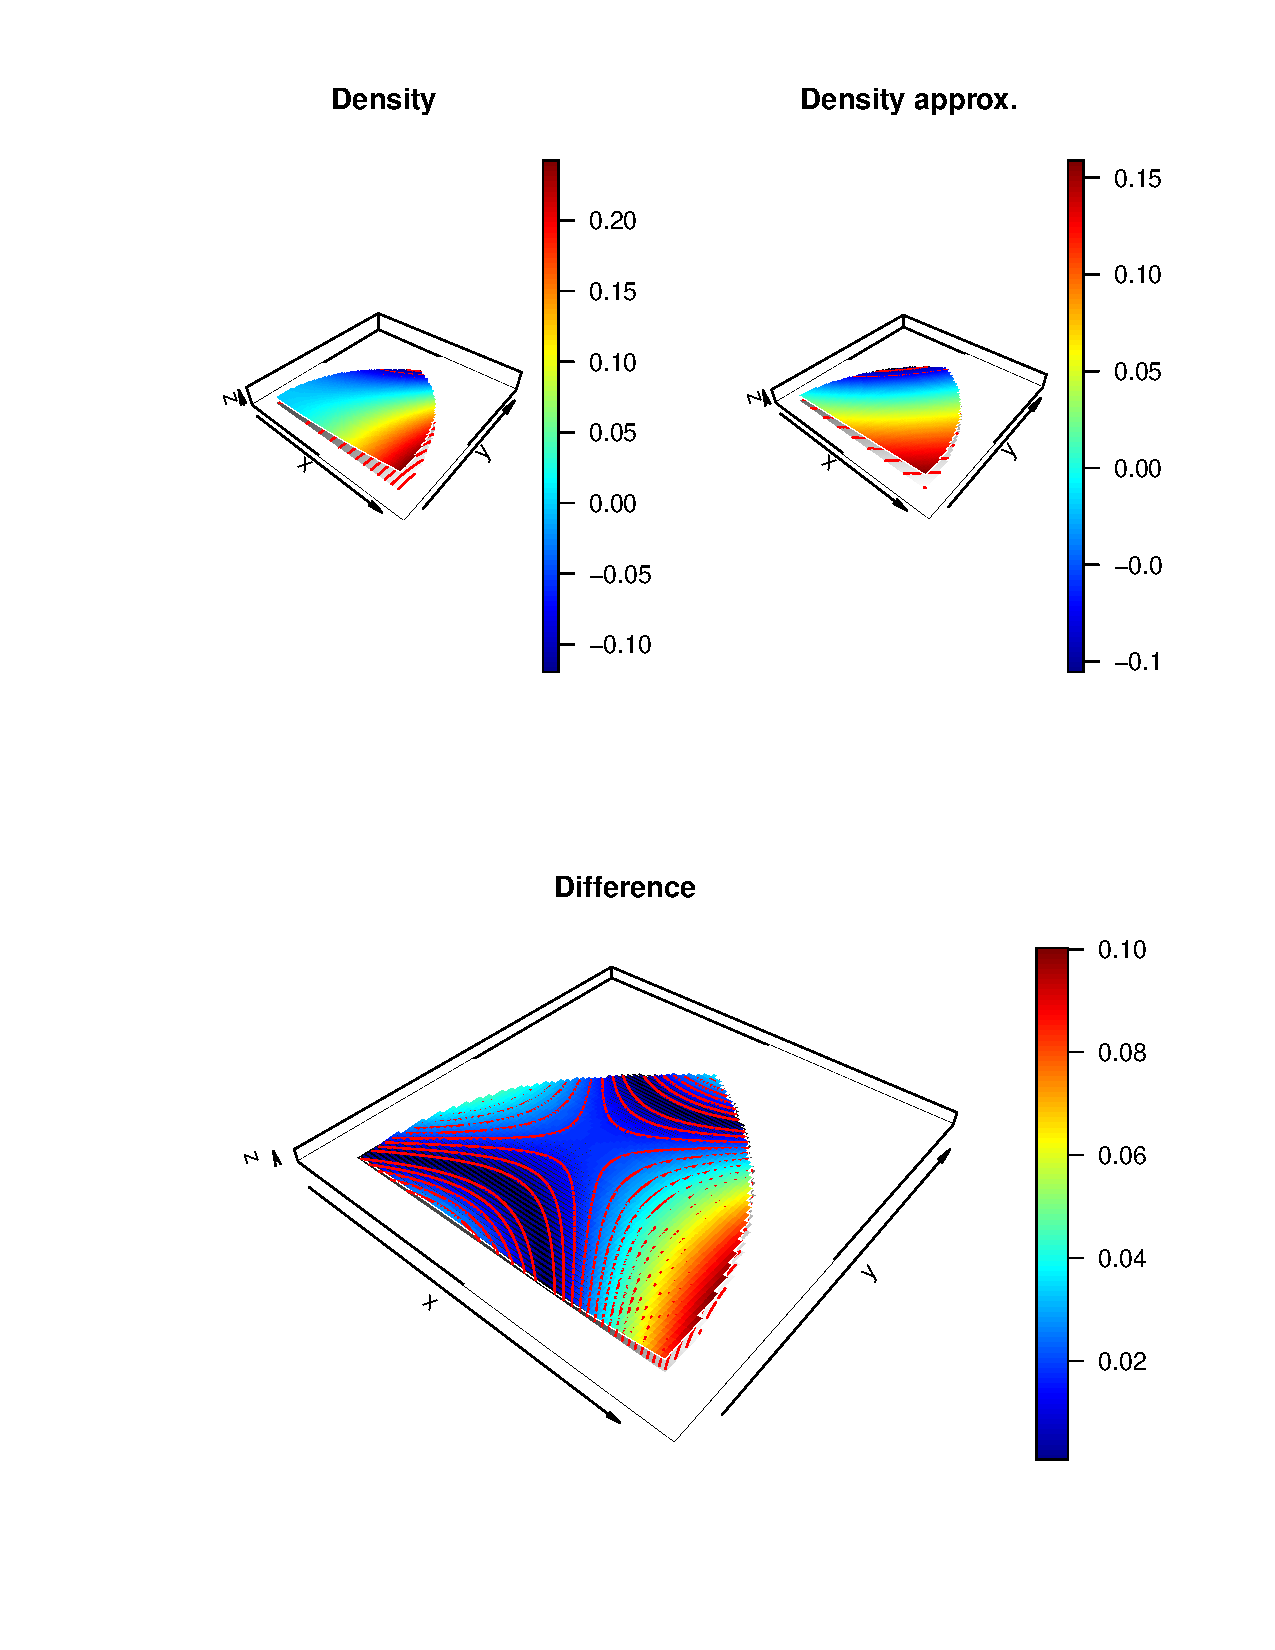
\includegraphics[width=0.95\linewidth]{f54.pdf}}
      \end{minipage}
      \caption{Для $f_5$}
      \label{ris:image1}
      \end{figure}

      \begin{figure}[h]
        \begin{minipage}[h]{0.49\linewidth}
        \center{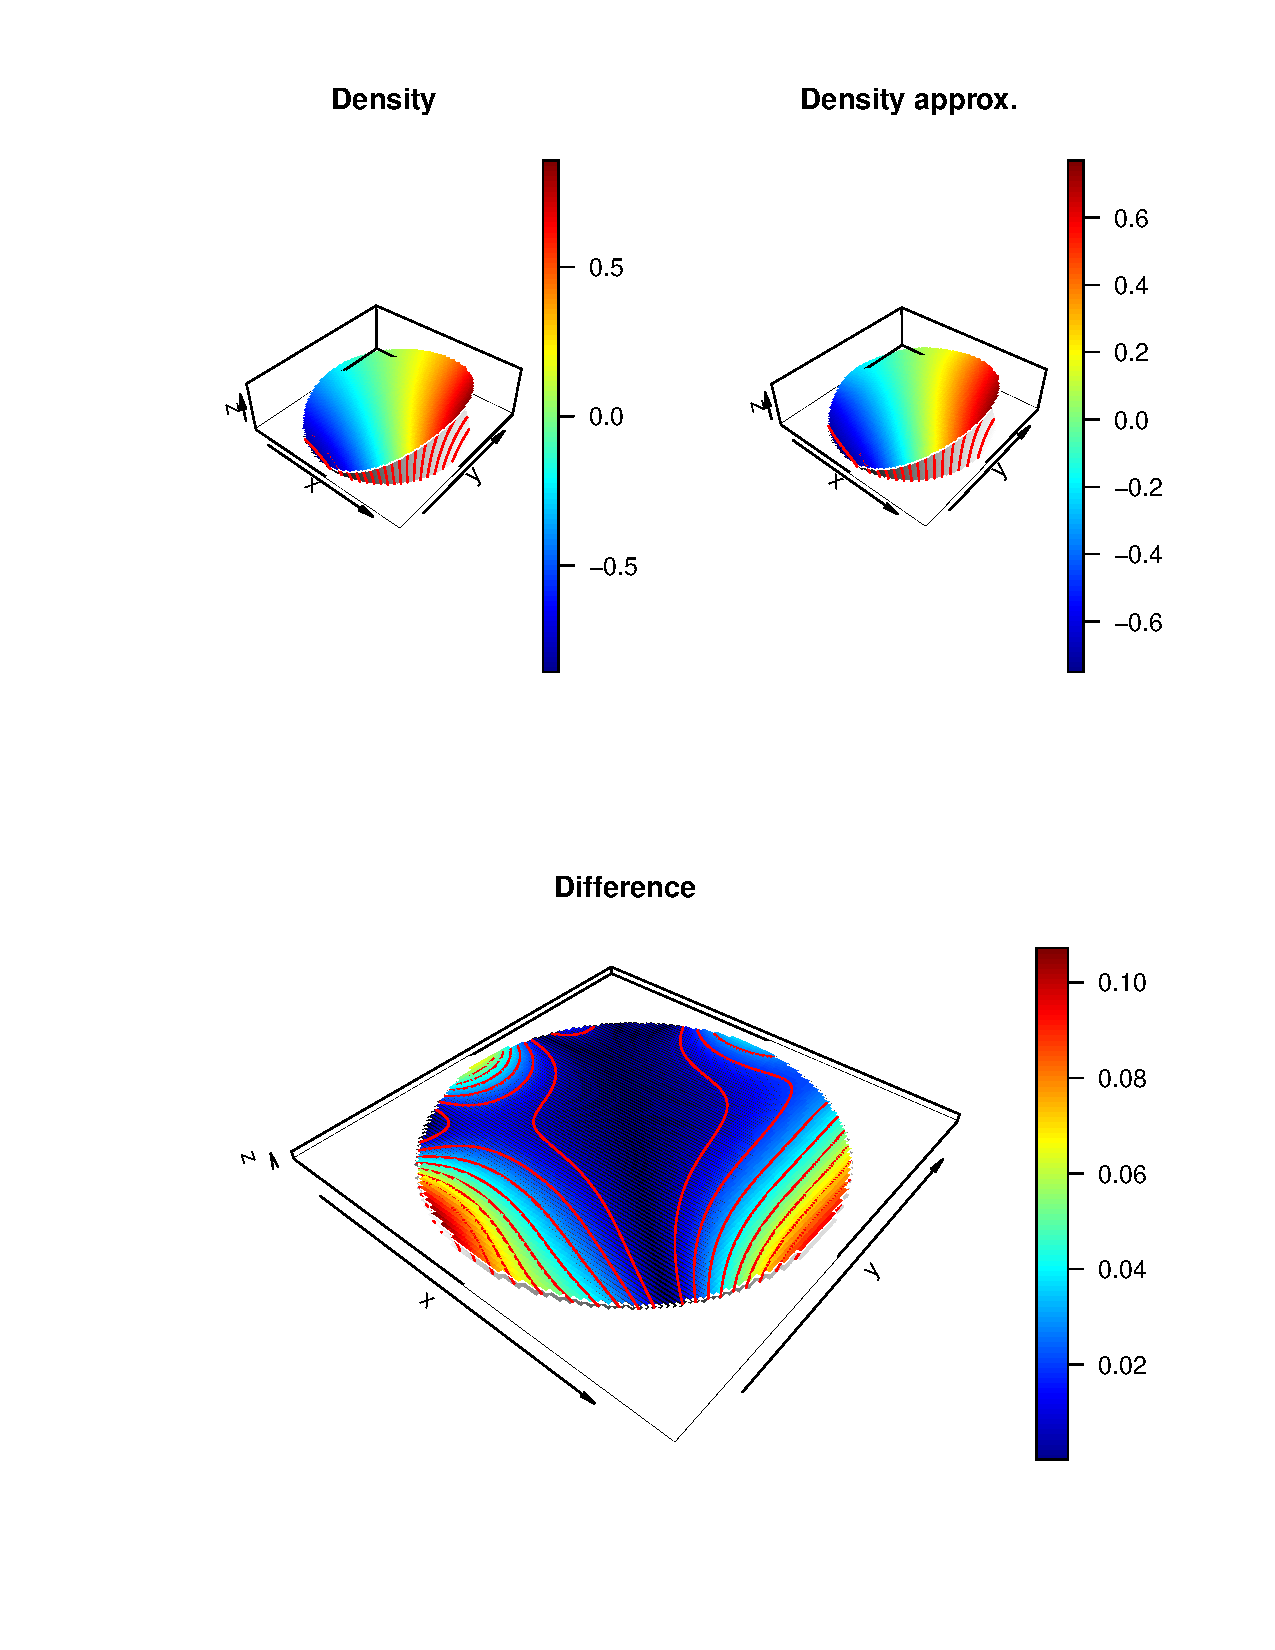
\includegraphics[width=0.95\linewidth]{f61.pdf}}
        \end{minipage}
        \hfill
        \begin{minipage}[h]{0.49\linewidth}
        \center{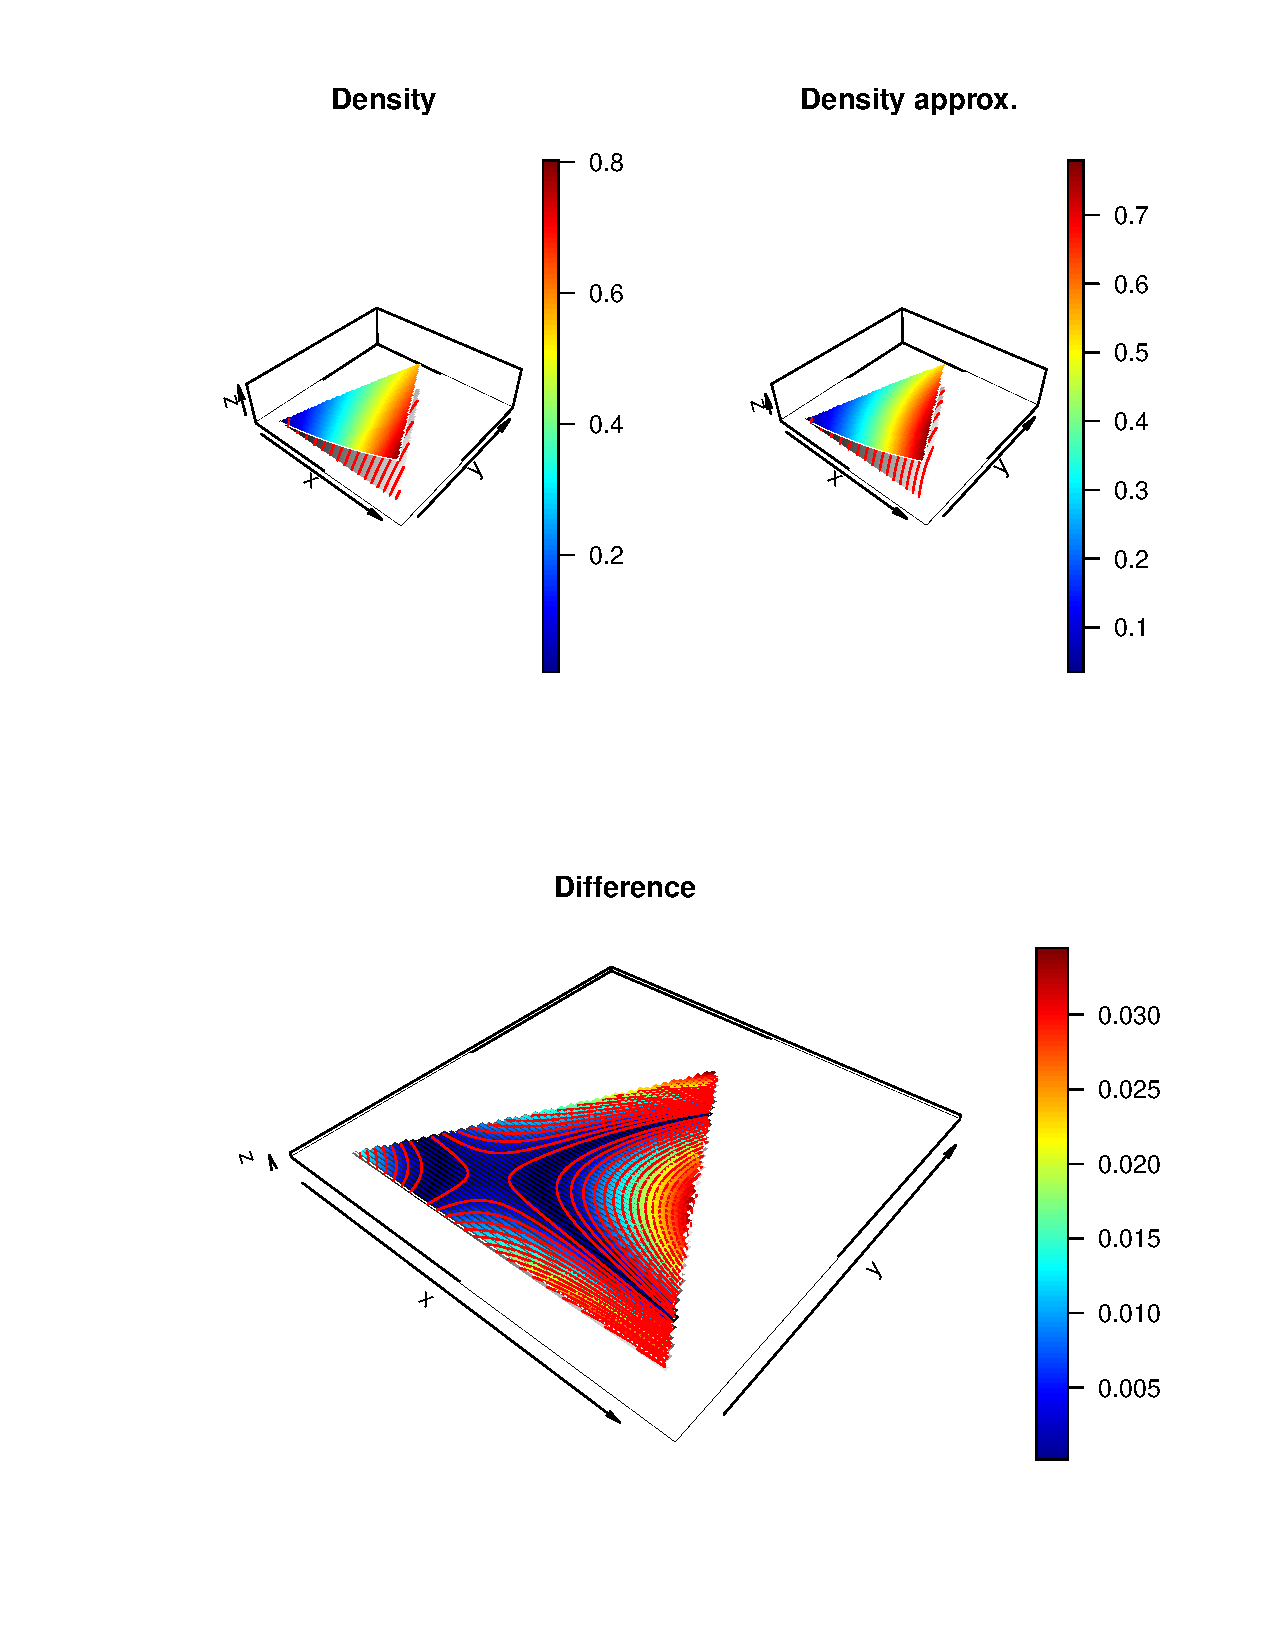
\includegraphics[width=0.95\linewidth]{f62.pdf}}
        \end{minipage}
        \caption{Для $f_6$}
        \label{ris:image1}
        \end{figure}

        \begin{figure}[h]
          \begin{minipage}[h]{0.49\linewidth}
          \center{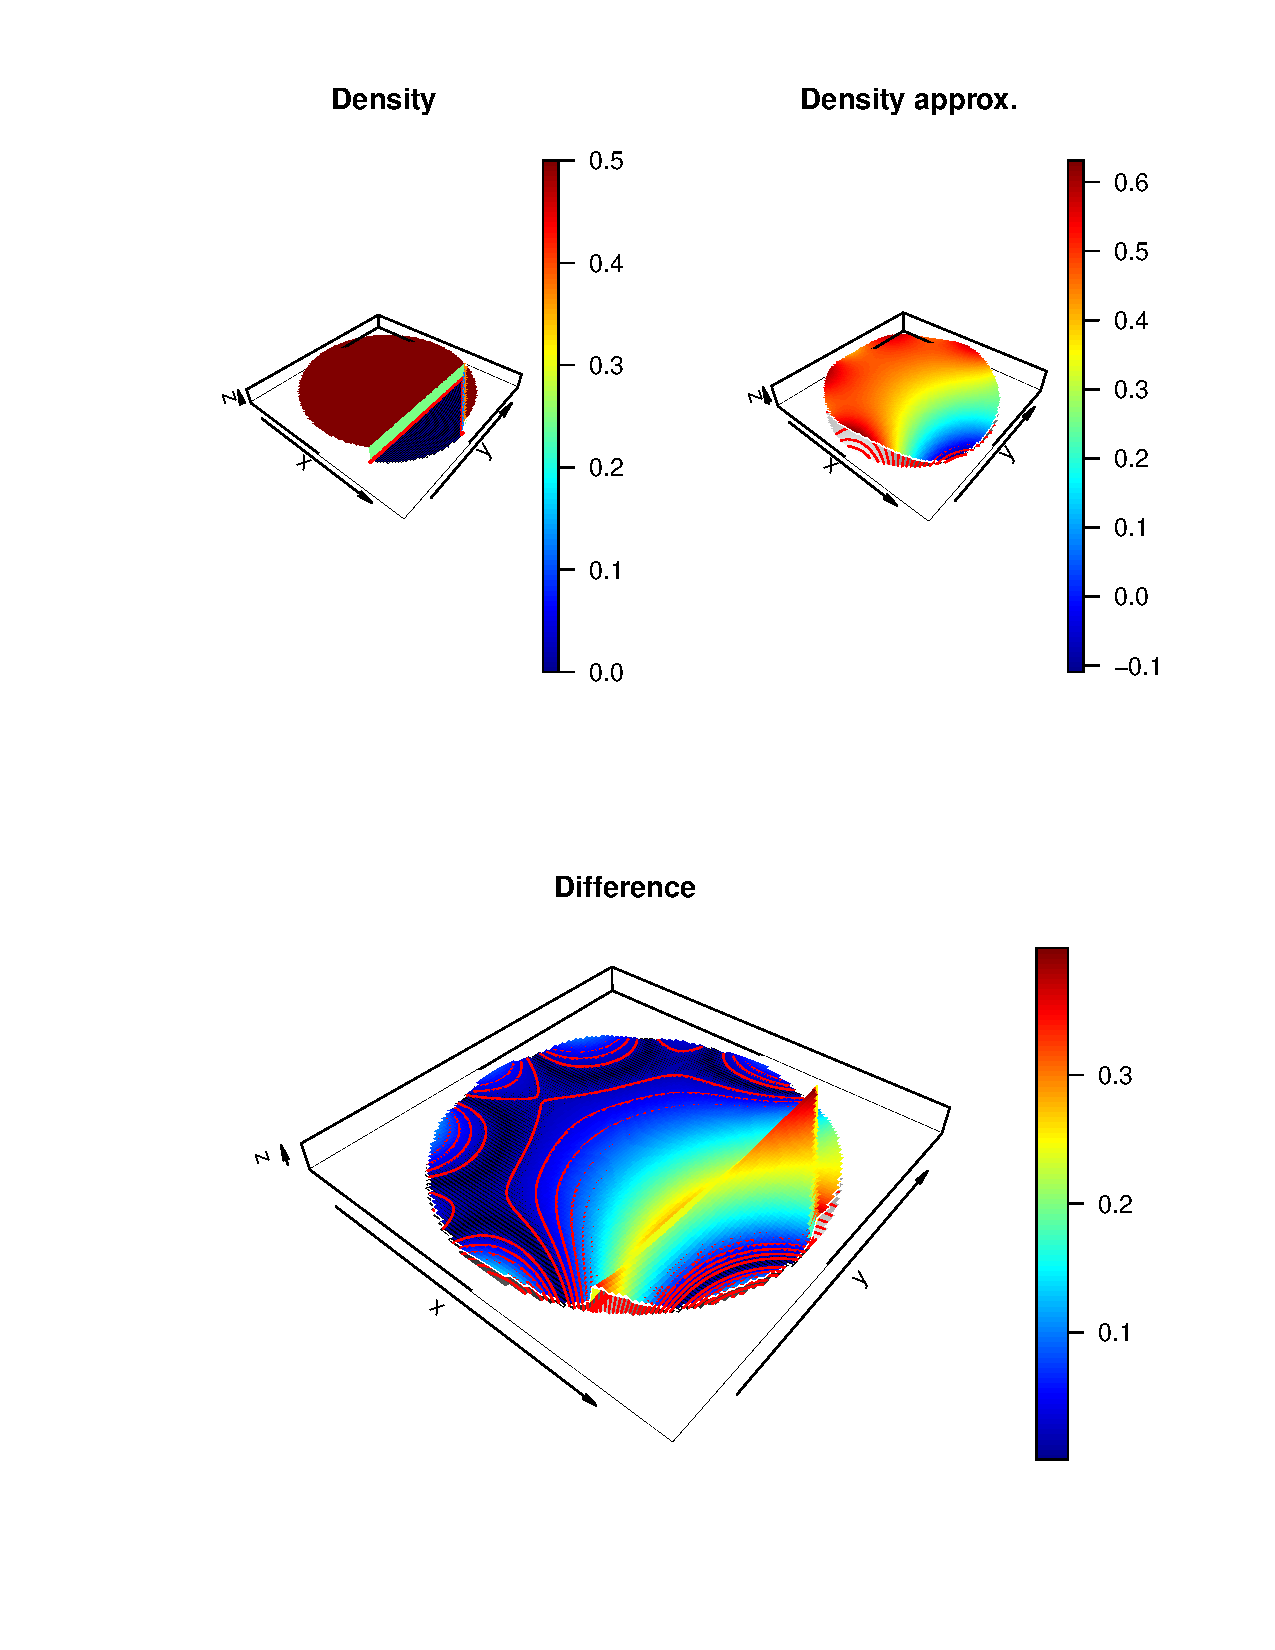
\includegraphics[width=0.95\linewidth]{f71.pdf}}
          \end{minipage}
          \hfill
          \begin{minipage}[h]{0.49\linewidth}
          \center{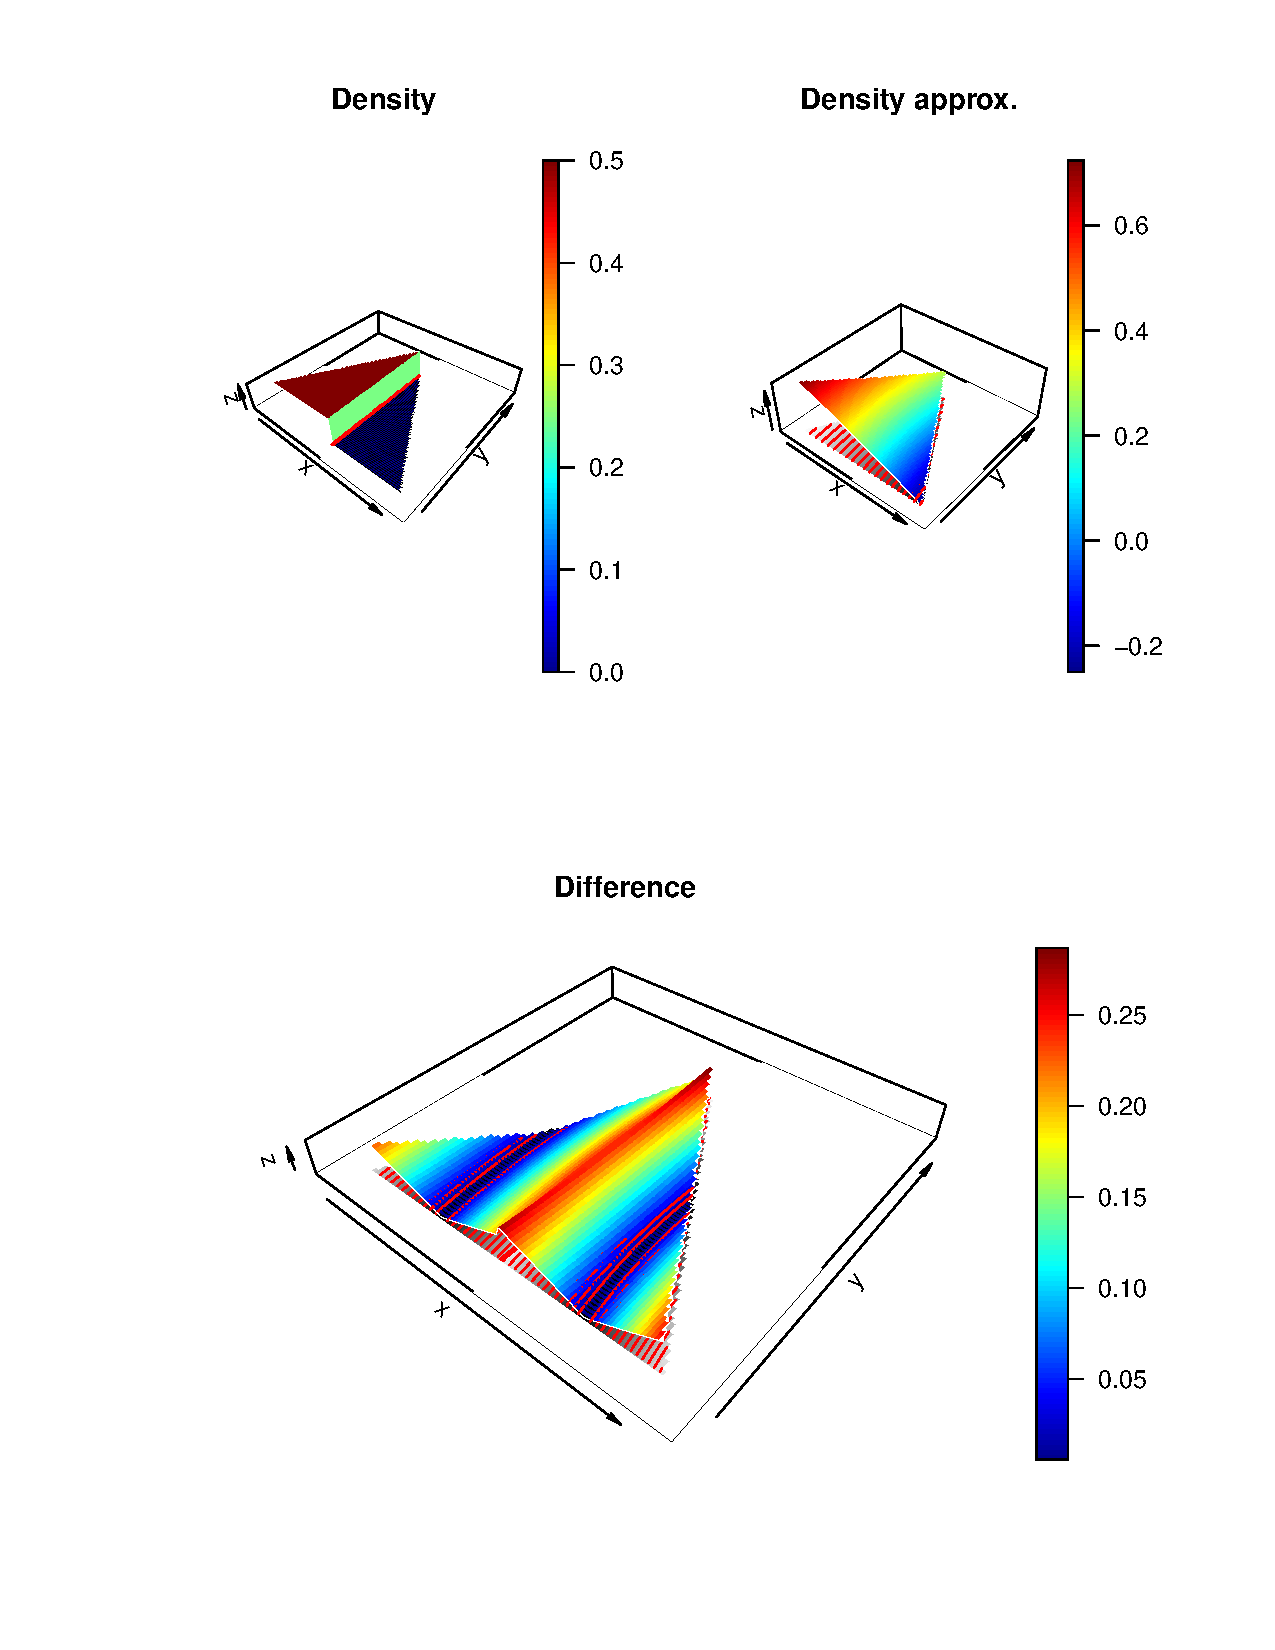
\includegraphics[width=0.95\linewidth]{f72.pdf}}
          \end{minipage}
          \caption{Для $f_7$}
          \label{ris:image1}
          \end{figure}

          \begin{figure}[h]
            \begin{minipage}[h]{0.49\linewidth}
            \center{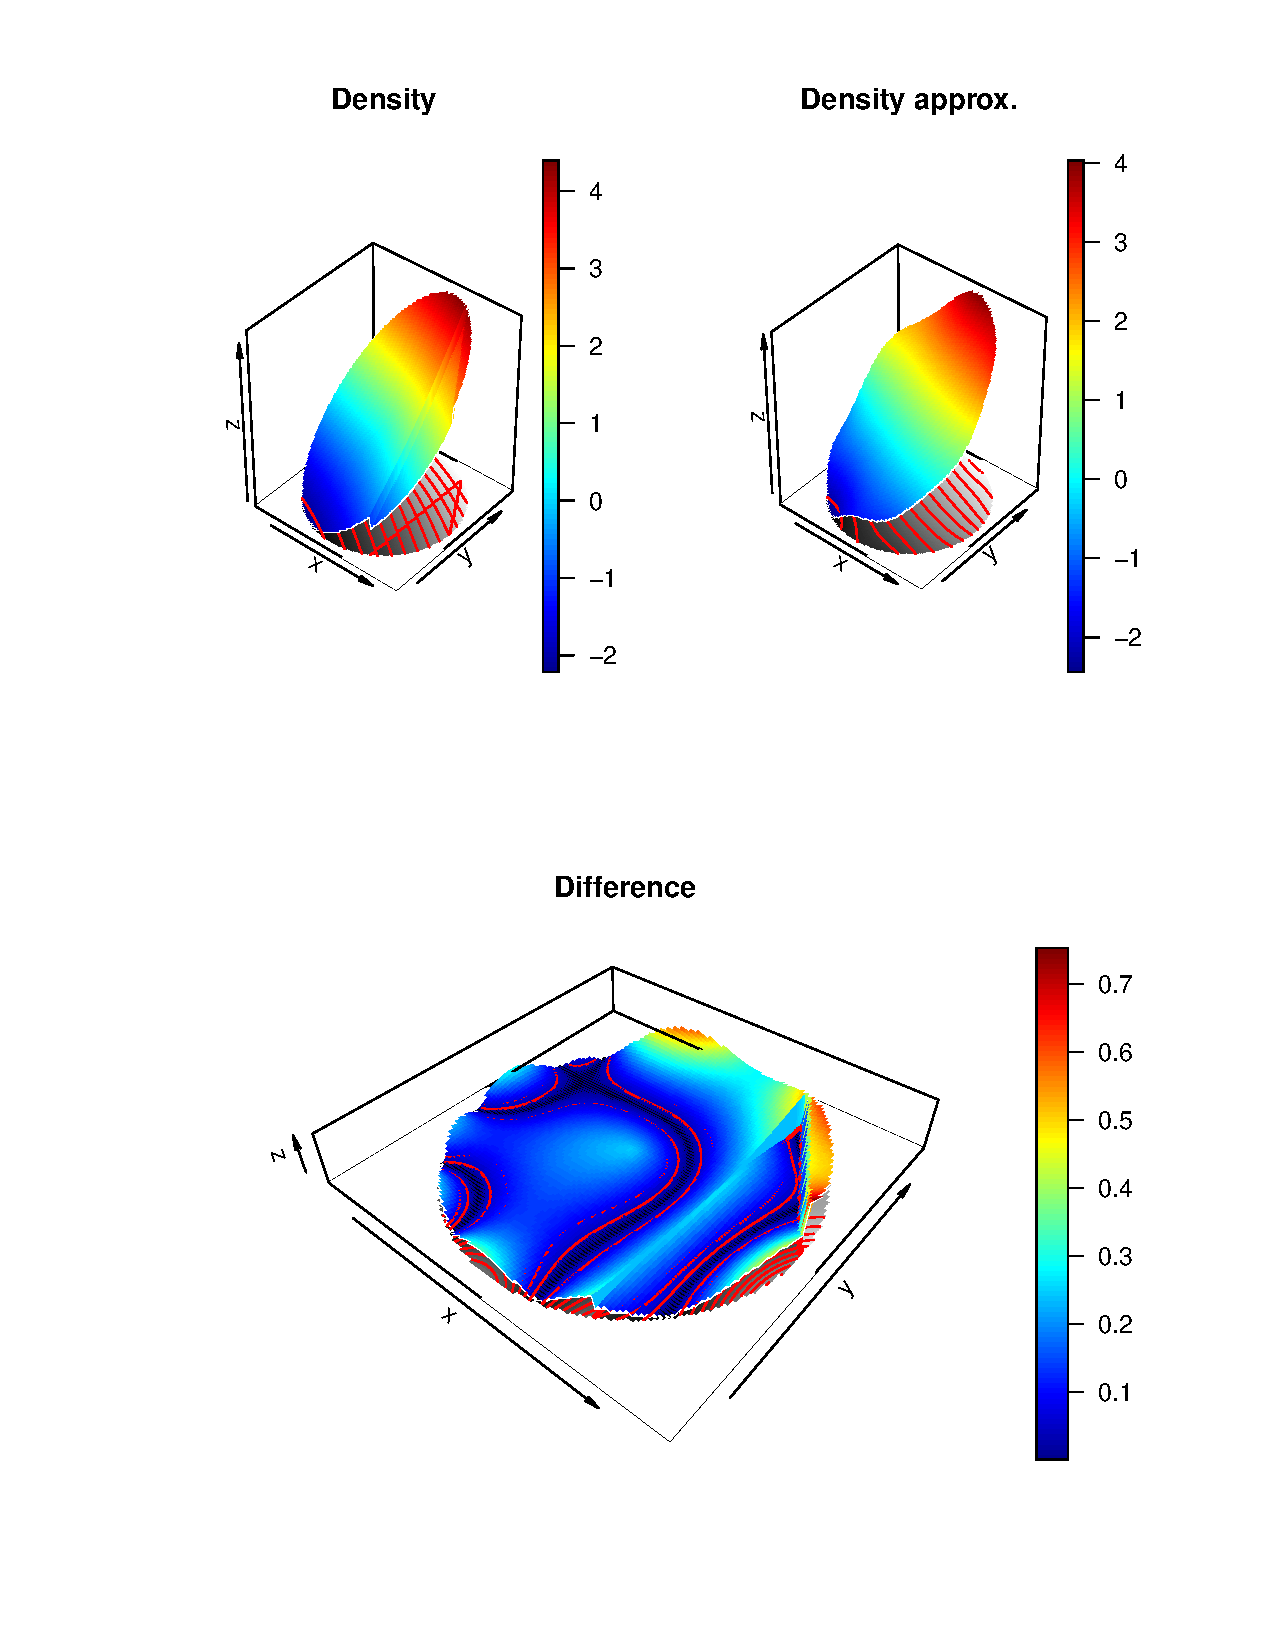
\includegraphics[width=0.95\linewidth]{f81.pdf}}
            \end{minipage}
            \hfill
            \begin{minipage}[h]{0.49\linewidth}
            \center{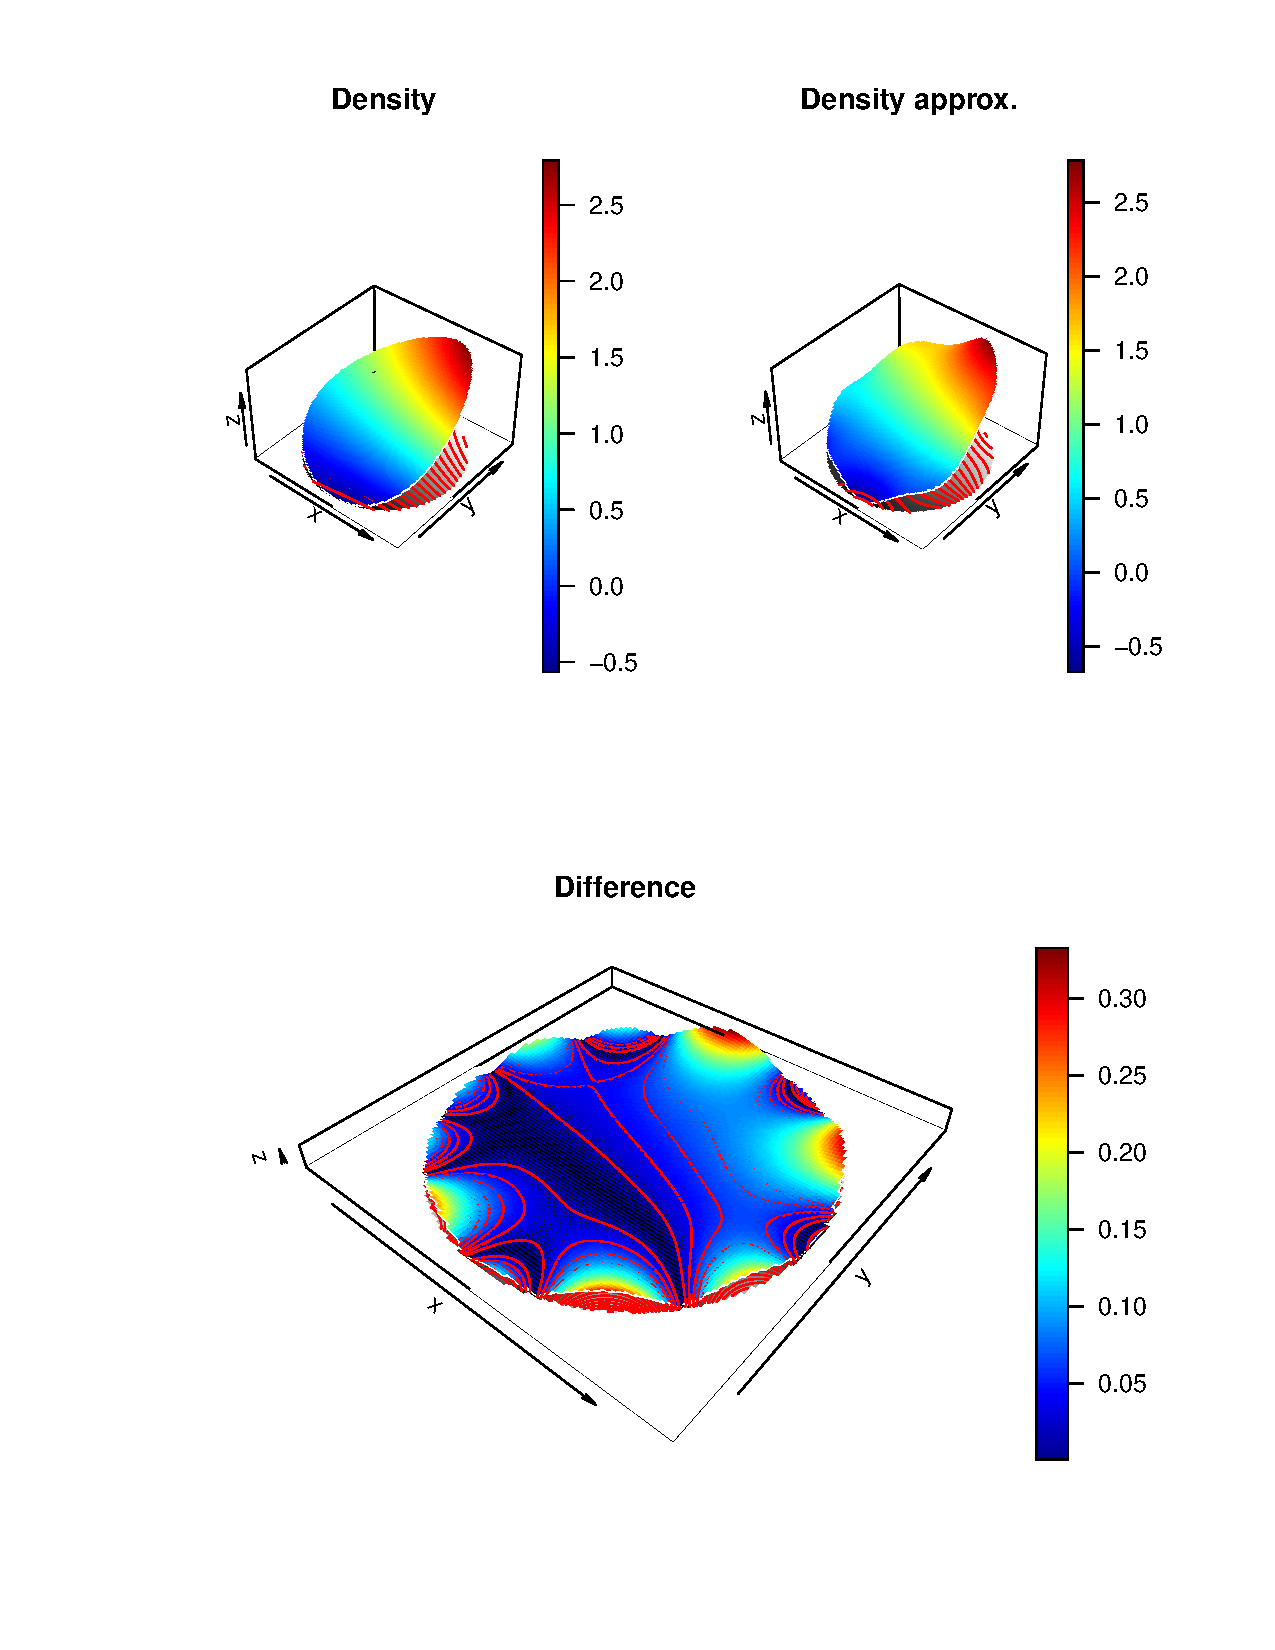
\includegraphics[width=0.95\linewidth]{f91.pdf}}
            \end{minipage}
            \caption{Для $f_8$ и $f_9$}
            \label{ris:image1}
            \end{figure}

              \begin{figure}[h]
                \begin{minipage}[h]{0.49\linewidth}
                \center{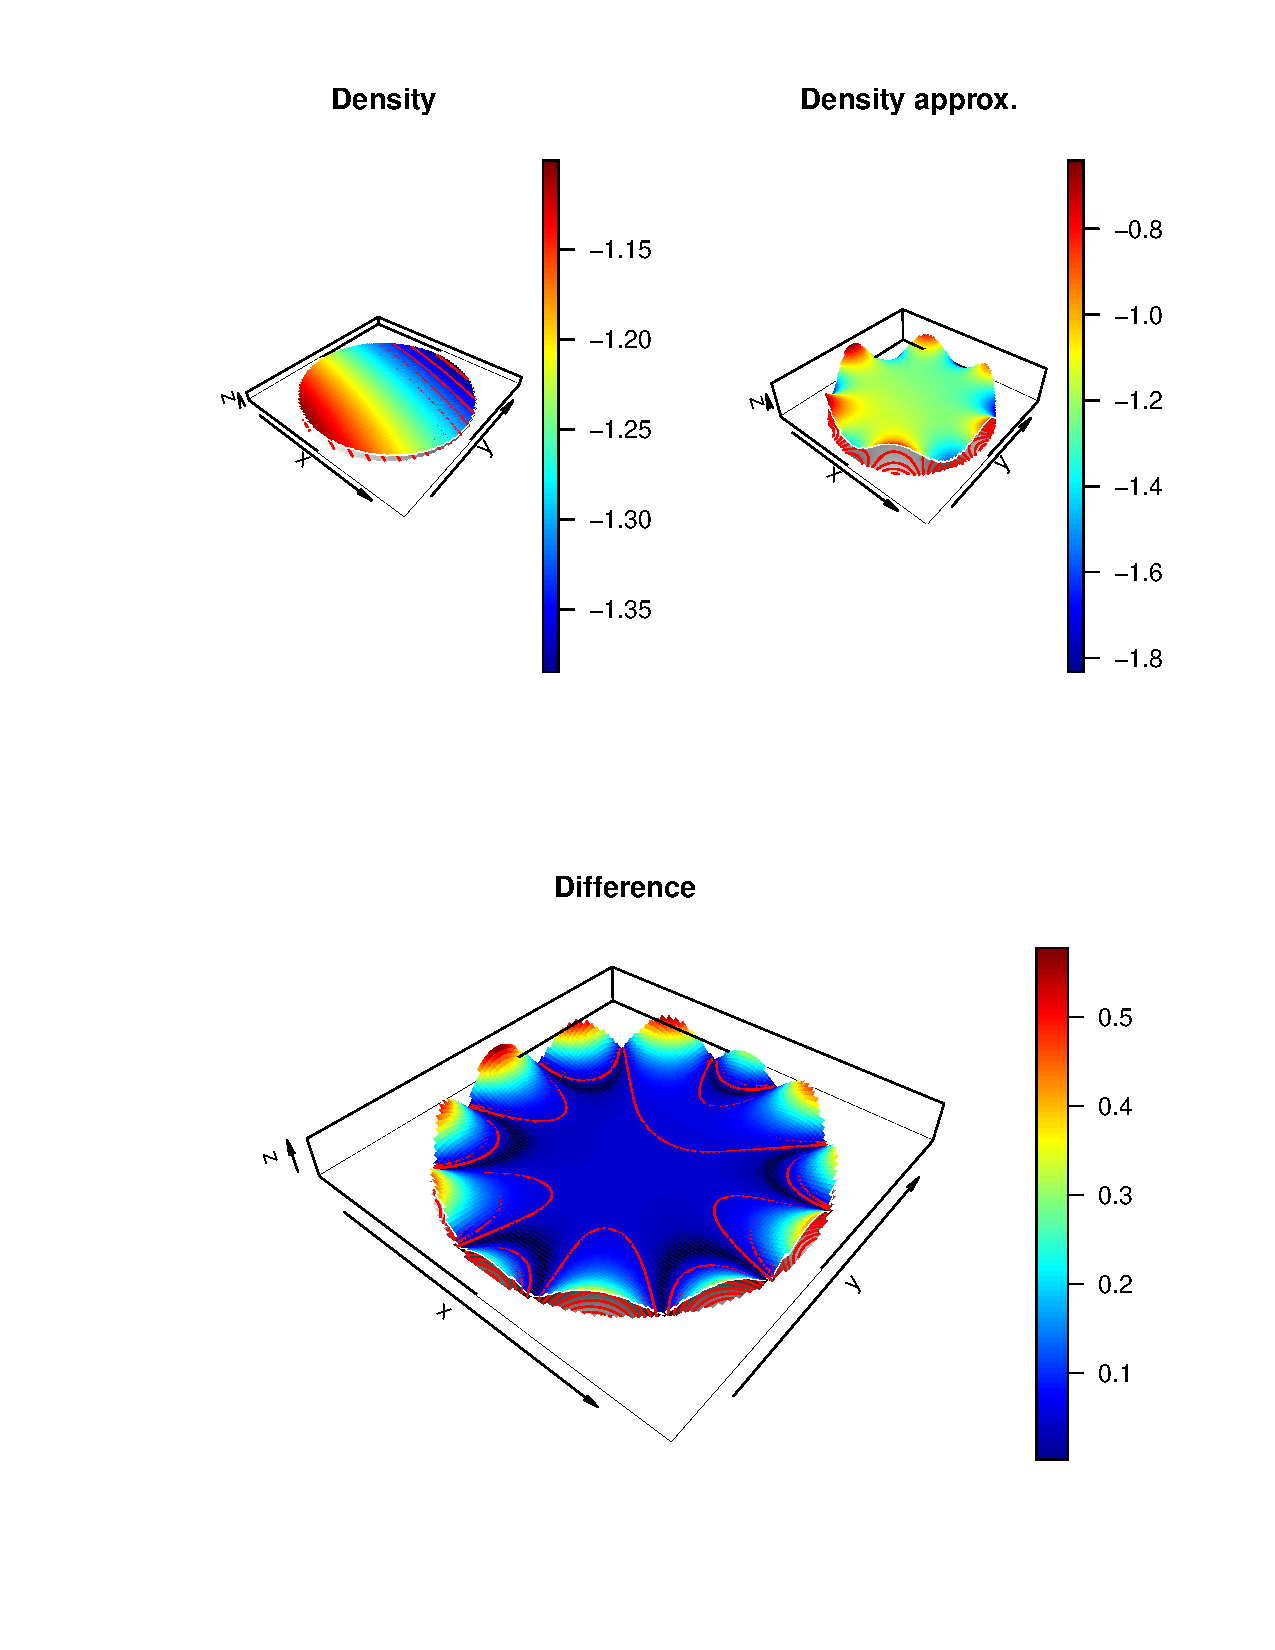
\includegraphics[width=0.95\linewidth]{f111.pdf}}
                \end{minipage}
                \hfill
                \begin{minipage}[h]{0.49\linewidth}
                \center{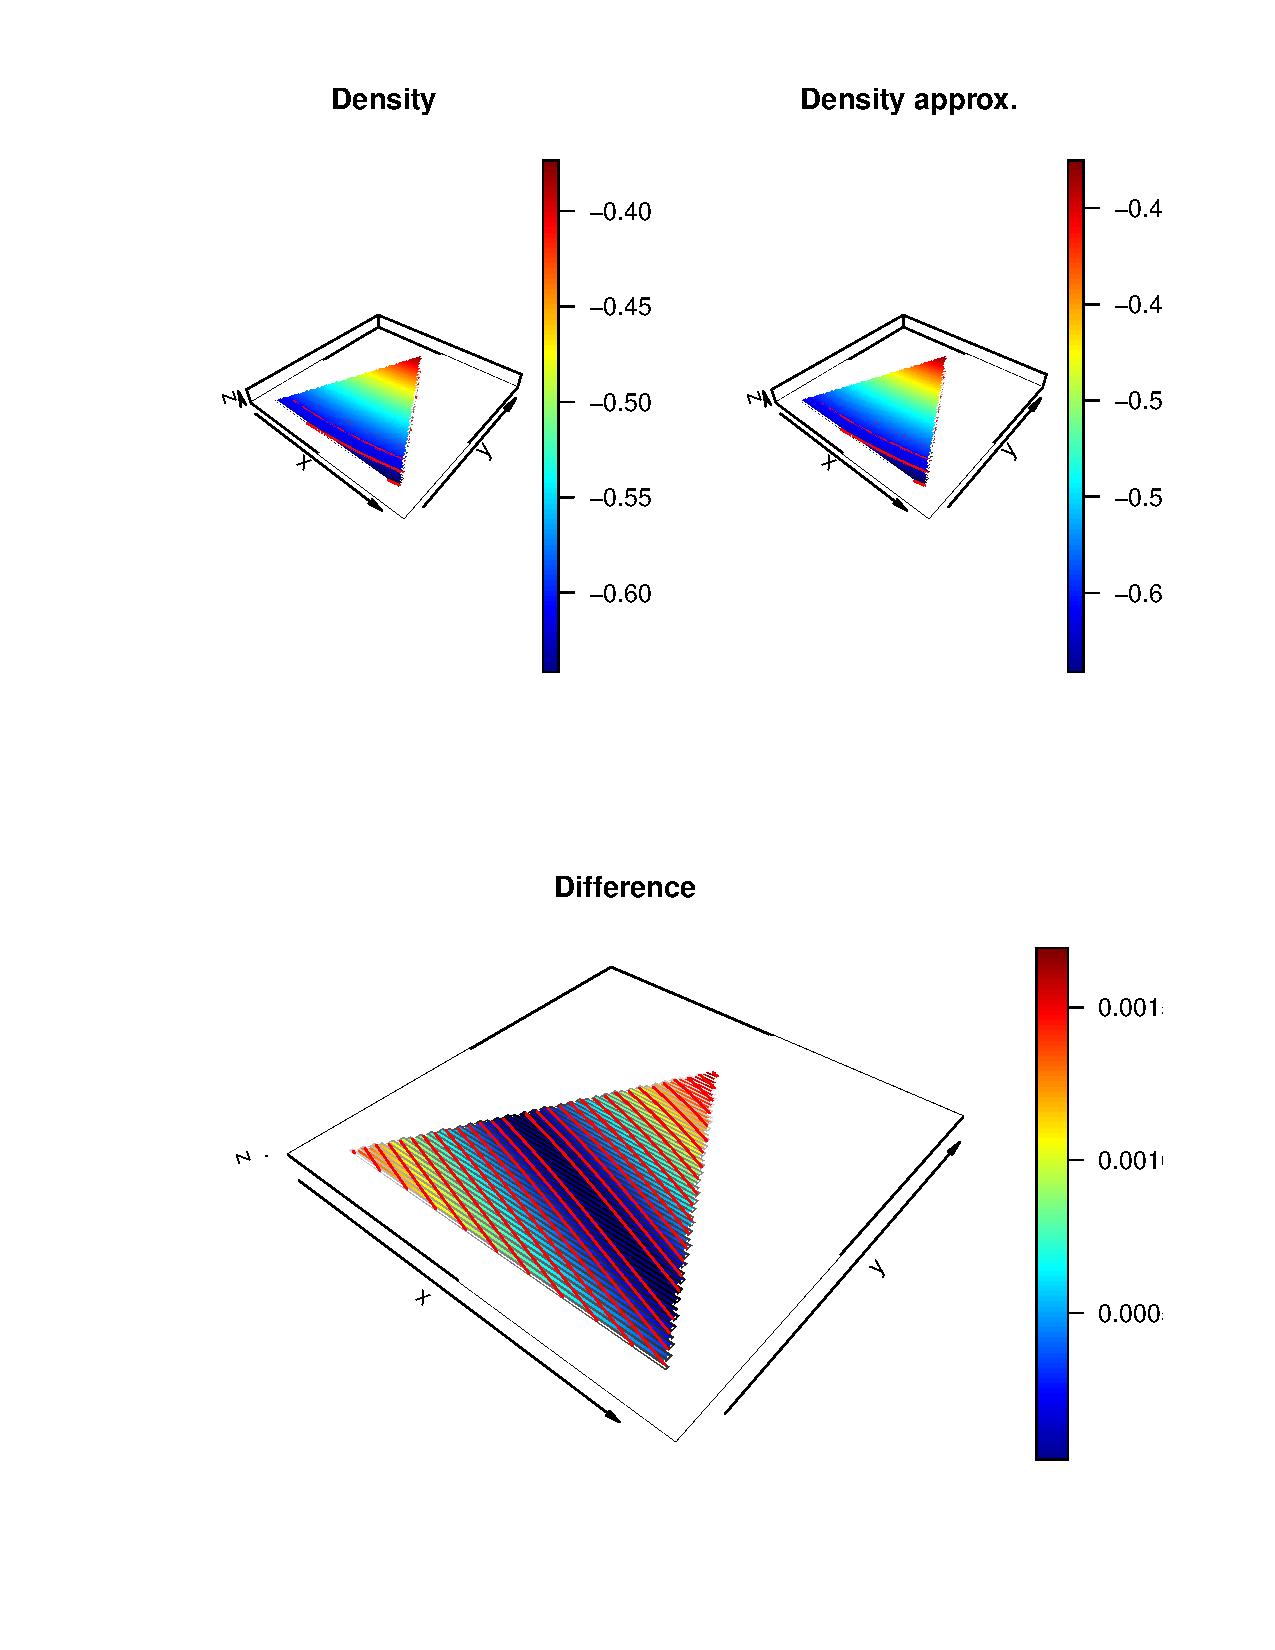
\includegraphics[width=0.95\linewidth]{f112.pdf}}
                \end{minipage}
                \caption{Для $f_{11}$}
                \label{d3end}
                \end{figure}
              
\FloatBarrier 
\subsection{Устойчивость решения ОЗГ в классе гармонических плотностей}
В этом разделе доказывается некорректность обратной задачи гравиметрии на примере системы плотностей из $\rho_k: \R{2}\rightarrow \mathbb{R}, k \in \mathbb{N}$.
Сначала формулируются понятие регулярного контура и относящиеся к нему утверждения, потом показывается оценка сверху для функций $V_{\rho_k}$, затем доказывается, что $V_{\frac{\rho_k}{||\rho_k||}} \rightarrow 0, k \rightarrow 0$, затем объясняется, почему это означает некорректность ОЗГ.

\subsubsection{О регулярных контурах}
Пусть
$V = \{V_{\rho} \in L_2(Q)\}, V \in C(\R{2})$ --- множество потенциалов,
\def\MYdef{\mathrel{\stackrel{\rm def}=}}
$V|_{\partial Q}\MYdef \{V_{\rho}|_{\partial Q}: \rho \in L_2(Q)\}$,
$V|_{\Gamma} \MYdef \{V_{\rho}|_{\Gamma}: \rho \in L_2(Q)\}$ --- сужение этих потенциалов на $\partial Q$ и некоторую кривую $\Gamma$,
и пусть имеется отношение эквивалентности между этими сужениями:
$$a \in V|_{\partial Q} \simeq b \in V|_{\Gamma}: \exists \rho \in L_2(Q):V|_{\partial Q}=a,V|_{\Gamma}=b.$$

По аналогии с результатами \cite{svid} выводятся следующие утверждения.

{\bf Утверждение 1}. Ядро отображения $\rho \in L_2(Q) \rightarrow V_{\rho}|_{\Gamma}, \rho \in G(Q)$ не более чем одномерно.

\begin{Proof}
  Пусть есть две разные функции из ядра: $V_{\rho_1}|_{\Gamma}=V_{\rho_2}|_{\Gamma}=0$.

{\bf Случай А}. $$\rho_1 \bot 1 \text{ в } L_2(Q) \Rightarrow V_{\rho_1} \rightarrow 0, x \rightarrow \infty \Rightarrow V_{\rho_1}=0 \text{ в } \Gamma^+ \Rightarrow V_{\rho_1}=0 \text{ в $\R{2}\backslash Q$},$$
поскольку $V_{\rho_1}$ аналитическая и тогда все её производные равны 0 на аналитических продолжениях, поэтому из леммы Новикова $\rho_1 \in N(Q)$.

{\bf Случай Б}. $$\rho_1 \not\bot 1, \rho_2 \not\bot 1 \Rightarrow \exists c\in R: \rho_3=\rho_1+c\rho_2 \bot 1 \text{ в } L_2(Q) \Rightarrow \rho_3 \in N(Q), \text{ чего не может быть.}$$
\end{Proof}

{\bf Утверждение 2}. Ядро отображения $\rho \in L_2(Q) \bigcap G(Q)\rightarrow V_{\rho}|_{\Gamma} \bigcap z_0, z_0 \in \Gamma^+$ -- тривиально. Доказательство следует из усиленного принципа максимума (опираясь на факт, что $z_0$ не может быть экстремумом).

{\bf Следствие}. Для двух контуров $\Gamma_1, \Gamma_2$ ядра не совпадают.

{\bf Определение}. Будем называть $\Gamma$ регулярным, если ядро отображения $\rho \rightarrow V_{\rho}|_{\Gamma}$ тривиально.

Суть этих утверждений в том, что все контуры $L$, подобные $\partial Q$, кроме одного, являются регулярными, то есть обеспечивают биективность отображения $\rho \rightarrow V_{\rho}|_{\Gamma}$.

\subsubsection{Вывод $V_{\rho_k}$}
Отождествим пока $\R{2}$ с комплексной плоскостью $\mathbb{C}$ и рассмотрим последовательность плотностей вида $\rho_k=\text{Re}\ z^k=r^k \cos k\varphi$.
Вычислим $V_{\rho_k}$ для $x=(z \cos\alpha,z \sin \alpha) \equiv z \cos\alpha + i z \sin \alpha$ вне области $Q= \{x \in \R{2}: |x|<1 \}$:
\begin{multline}
    V_{\rho_k}(x)= \int_Q \rho_k(y) E(x-y) dy= \int_0^1 \int_0^{2 \pi} r^k \cos k\varphi \ln |x-(r \cos \varphi, r \sin\varphi)| r d\varphi dr =\\
\Bigl|\alpha = \text{Arg}\ x, z=|x| \Bigl|=
\int_0^1 \int_0^{2 \pi} r^{k+1} \cos k\varphi \ln \sqrt{(z\cos \alpha-r \cos \varphi)^2+(z\sin \alpha-r \sin\varphi)^2} d\varphi dr=\\
\frac{1}{2} \int_0^1 \int_0^{2 \pi} r^{k+1} \cos k\varphi \ln(z^2 - 2z r \cos\varphi \cos \alpha +(r \cos \varphi)^2 - 2z r \sin \varphi \sin \alpha +(r \sin \varphi)^2) d\varphi dr =\\
\frac{1}{2} \int_0^1 \int_0^{2 \pi} r^{k+1} \cos k\varphi \ln(z^2-2zr(\cos \varphi \cos \alpha + \sin \varphi \sin \alpha)+r^{2})d\varphi dr=\\
\frac{1}{2} \int_0^1 r^{k+1}\int_0^{2 \pi}  \cos k\varphi \ln(z^2 + r^{2} - 2zr \cos (\varphi -\alpha)) d\varphi dr=\\
\frac{1}{2} \int_0^1 r^{k+1}\int_0^{2 \pi}\cos (k(\varphi -\alpha)+k\alpha)\ln(z^2 + r^{2} - 2zr \cos (\varphi -\alpha)) d\varphi dr= \\
\frac{1}{2} \int_0^1 r^{k+1}\int_0^{2 \pi}\left(\cos (k(\varphi -\alpha)) \cos(k\alpha) - \sin (k(\varphi -\alpha)) \sin(k\alpha)\right) \ln(z^2 + r^{2} - 2zr \cos (\varphi -\alpha)) d\varphi dr=\dots
\end{multline}

Рассмотрим интеграл $$\int_0^{2\pi} \sin (k(\varphi -\alpha)) \sin(k\alpha) \ln(z^2 + r^{2} - 2zr \cos (\varphi -\alpha)) d \varphi.$$
Поскольку функция $\sin (k(\varphi -\alpha))$ нечётна по $\varphi$, а $\cos(\varphi - \alpha)$ чётна по $\varphi$, то подинтегральная функция нечётна как произведение чётной и нечетной функций.
А поскольку $\sin (k(\varphi -\alpha))$ $ \frac{2\pi}{k}$-периодична, $k \in \mathbb{N}$, $\cos(\varphi - \alpha)$ --- $2\pi$-периодична, то указанный интеграл обращается в ноль как интеграл от нечётной периодической функции на периоде. Искомый интеграл упрощается:
\begin{multline}
   \dots =\frac{1}{2} \int_0^1 r^{k+1}\cos(k\alpha)\int_0^{2 \pi}\cos (k(\varphi -\alpha))  \ln(z^2 + r^{2} - 2zr \cos (\varphi -\alpha)) d\varphi dr=\\
   \frac{1}{2} \cos(k\alpha) \int_0^1 r^{k+1}\int_0^{2 \pi}\cos (k(\varphi -\alpha))  \ln(z^2 + r^{2} - 2zr \cos (\varphi -\alpha)) d(\varphi-\alpha) dr =\Bigl|\text{выполняем замену $\tau=\varphi - \alpha$}\Bigl|=\\
   \frac{1}{2} \cos(k\alpha) \int_0^1 r^{k+1}\int_{-\alpha}^{2 \pi - \alpha}\cos (k \tau)  \ln(z^2 + r^{2} - 2zr \cos \tau) d\tau dr =\Bigl| \text{в силу периодичности}\Bigl|=\\
   \frac{1}{2} \cos(k\alpha) \int_0^1 r^{k+1}\int_{0}^{2 \pi}\cos (k \tau)  \ln(z^2 + r^{2} - 2zr \cos \tau) d\tau dr=\\
   \frac{1}{2} \cos(k\alpha) A_k(z),
\end{multline}
где
\begin{equation}
    A_k(z)=\int_0^1 r^{k+1}\int_{0}^{2 \pi}\cos (k \tau)  \ln(z^2 + r^{2} - 2zr \cos \tau) d\tau dr.
\end{equation}

Заметим, что $A_k(z)$ ограничена:
\begin{multline}
    |A_k(z)| \leq \int_0^1 r^{k+1}\int_{0}^{2 \pi}|\cos (k \tau)|  \bigl|\ln(z^2 + r^{2} - 2zr \cos \tau)\bigl| d\tau dr \\
    \leq \int_0^1 r^{k+1}\int_{0}^{2 \pi}\bigl|\ln(z^2 + r^{2} - 2zr \cos \tau)\bigl| d\tau dr
    \leq  2\pi \int_0^1 r^{k+1} \max \left(\Bigl| \ln ((z-r)^2) \Bigl|, \Bigl| \ln ((z+r)^2) \Bigl| \right)dr \\
    \leq 2\pi \int_0^1 r^{k+1} \sup_{t \in S_r(z)} \bigl| \ln (t^2) \bigl|dr \leq 2\pi \sup_{t \in B_1(z)} \bigl| \ln (t^2) \bigl| \int_0^1 r^{k+1} dr =2\pi  \frac{\sup_{t \in B_1(z)} \bigl| \ln (t^2) \bigl|}{k+2}.
\end{multline}
Здесь под $S_r(z) \subset \mathbb{R} $ подразумевается окружность радиуса $r$ с центром в $z$, под $B_1(z) \subset \mathbb{R}$ --- шар единичного радиуса с центром в $z$. Ясно, что это сокращённое обозначение для концов отрезка $[z-r, z+r]$ и самого отрезка $[z-1,z+1]$ соответственно.

Из приведённых выкладок следует, что 
\begin{equation}
   | V_{\rho_k}(x)| \leq \pi \frac{\sup_{t \in B_1(z)} \bigl| \ln (t^2) \bigl|}{k+2},
\end{equation}
то есть для $V_{\rho_k}$ найдена оценка сверху. На рисунке \ref{chis} эта оценка подтверждается численно.
\begin{figure}[h!]
  \noindent\centering{
  \includegraphics[width=\linewidth]{valargs.pdf}
}
  \caption{Разность $\pi \frac{\sup_{t \in B_1(z)} \bigl| \ln (t^2) \bigl|}{k+2} -| V_{\rho_k}(x)| $ для разных $k$}
  \label{chis}
  \end{figure} 

\subsubsection{Некорректность ОЗГ}
Пусть, как и в предыдущем пункте, $Q$ --- единичный шар, а потенциал считается на поверхности $S: \{x\in \R{2}: |x|=2 \}$. В таком случае
\begin{multline}
    ||\rho_k ||_{L_2(Q)}=\sqrt{\int_0^1 \int_0^{2 \pi} r^{2k} \cos^2(k \varphi) d\varphi dr}= \sqrt{\int_0^1 r^{2k} \int_0^{2 \pi} \frac{\cos(2k \varphi)+1}{2}  d\varphi dr}\\
    =\sqrt{\frac{1}{2} \int_0^1 r^{2k} \left( \frac{\sin(2k \varphi)}{2k} +\varphi\right)\Biggl|_0^{2 \pi} dr}= \sqrt{\pi \int_0^1 r^{2k} dr}=\sqrt{\frac{\pi}{2k+1}}.
\end{multline}

Тогда
\begin{multline}
    \Bigl|\Bigl|V_{\frac{\rho_k}{||\rho_k ||}}  \Bigl|\Bigl|_{C(S)}= \frac{1}{||\rho_k ||} \Bigl|\Bigl|V_{\rho_k}  \Bigl|\Bigl|_{C(S)} \leq \sqrt{\frac{2k+1}{\pi}} \max_{x \in S} \Bigl| V_{\rho_k}(x) \Bigl| \leq \sqrt{\frac{2k+1}{\pi}} \pi |\cos(k\alpha)| \frac{\sup_{t \in B_1(2)} \bigl| \ln (t^2) \bigl|}{k+2} \\
    \leq \sqrt{\frac{2k+1}{\pi}} \pi \frac{\sup_{ t \in B_1(2)} \bigl| \ln (t^2) \bigl|}{k+2} = \sqrt{\pi} \sqrt{\frac{2k+1}{k^2 + 4k+4}}\sup_{t \in B_1(2)} \bigl| \ln (t^2) \bigl| \xrightarrow{k \rightarrow \infty} 0.
\end{multline}

Итак, ранее доказано, что $$\Bigl|\Bigl|V_{\frac{\rho_k}{||\rho_k ||}}  \Bigl|\Bigl|_{C(S)}\xrightarrow{k \rightarrow \infty} 0.$$
Представим $V$ как линейный оператор: $V: L_2(Q) \bigcap G(Q) \rightarrow C(S)$. Пусть $S$ --- такая поверхность, что $\text{Ker} (V)=\{0\}$ (то есть регулярный контур);
тогда существует обратный оператор $V^{-1}$.
Рассмотрим образ $V^{-1}$ на единичной сфере $\frac{V\left(\frac{\rho_k}{||\rho_k ||}\right)}{||V\left(\frac{\rho_k}{||\rho_k ||}\right)||}$:
\begin{equation}
  V^{-1}\left(\frac{V\left(\frac{\rho_k}{||\rho_k ||}\right)}{\Bigl|\Bigl|V\left(\frac{\rho_k}{||\rho_k ||}\right)\Bigl|\Bigl|}\right)=\frac{\frac{\rho_k}{||\rho_k ||}}{\Bigl|\Bigl|V\left(\frac{\rho_k}{||\rho_k ||}\right)\Bigl|\Bigl|} \xrightarrow{k\rightarrow \infty} \infty,
\end{equation}
поскольку $\Bigl|\Bigl|\frac{\rho_k}{||\rho_k ||}\Bigl|\Bigl|_{L_2(Q)}=1$ и $\Bigl|\Bigl|V_{\frac{\rho_k}{||\rho_k ||}}  \Bigl|\Bigl|_{C(S)}\xrightarrow{k \rightarrow \infty} 0$.
Значит, оператор $V^{-1}$ неограничен, что и означает некорректность\footnote{Из неограниченности обратного оператора следует, что из-за малых погрешностей на области значений оператора могут появляться огромные погрешности на его области определения.}.

\subsection{Демонстрация неустойчивости}
В этом разделе будут показаны примеры из практики, демонстрирующие неустойчивость ОЗГ.
\subsubsection{Пояснения о неустойчивости и реализации решения}
Опираясь на пояснения из раздела 3.1, зафиксируем вблизи кривой $L$ $n$ базисных потенциалов (точек).
Решив задачу минимизации функционала
\begin{equation*}
  F(c_1,\dots,c_k,\dots,c_n)=||V_{\rho}-V_{\sum_{i=1}^n c_i \alpha_i}||_{L_2(L)},
\end{equation*}
получим некоторый набор ${\bf c}=(c_1,\dots,c_k,\dots,c_n)$ и значение погрешности $\varepsilon_n = \varepsilon ({\bf c})$.
Ясно, что $\varepsilon$ должна не возрастать с ростом $n$, но только если рост $n$ происходит за счёт добавления новых точек в исходных набор базисных потенциалов (Рис. \ref{points2}),
поскольку разные точки вносят разный вклад в качество аппроксимации.
\begin{figure}[h!]
  \noindent\centering{
  \includegraphics[width=0.7\linewidth]{Points2.pdf}
}
  \caption{С ростом числа точек аппроксимация должна не ухудшаться, если только точки добавляются к уже зафиксированным}
  \label{points2}
  \end{figure} 

Если же при каждом новом $n$ все точки пересчитываются, мы имеем дело уже с разными задачами, чьи результаты не подходят для сравнения.

Чтобы обеспечить выполнение указанного условия, я изначально фиксировал вблизи кривой максимальное количество $n$ нужных для эксперимента точек,
затем случайным образом смешивал их индексы, чтобы точки, взятые по порядку, располагались не рядом друг с другом на кривой.
После этого сразу заполнялась система $n \times n$, причём для функций $\omega_i(x) =\V{\alpha_i}, i=1,\dots,n$ производилась мемоизация (запоминание результатов), что ускоряло заполнение системы в десятки раз, так как
фактически требовалось найти лишь $n$ элементов вместо $n(n-1)$.
Далее к уже готовой системе применялся ультра-гибрид.

Поскольку ультра-гибрид гарантирует устойчивую аппроксимацию, действительно выполнялось условие $\varepsilon_k \geq \varepsilon_{k+1}, k=1, \dots, n-1$ (устойчива аппроксимация $V_{\rho} \text{ на } L_2(L)$), однако при подстановке коэффициентов решения ${\bf c}_k, k=1,\dots,n$ в функционал
\begin{equation*}
  T({\bf c}_k)=\biggl|\biggl|\rho - \sum_{i=1}^k c_i \alpha_i\biggl|\biggl|_{L_2(Q)}=\epsilon_k,
\end{equation*}
условие $\epsilon_k \geq \epsilon_{k+1}, k=1, \dots, n-1$ более чем в половине случаев не выполнялось, то есть ультра-гибрид находил такие наборы коэффициентов ${\bf c}_k$, при которых
аппроксимация потенциала была устойчивой, а аппроксимация плотности --- нет, что и означает неустойчивость ОЗГ.
Кроме того, неустойчивость проявляется в том, что очень малые различия в начальных условиях (визуально прямые линии на графиках потенциалов --- на самом деле они содержат спуски в доли процентов) обращаются в заметные колебания на решении (скачки на графиках аппроксимации плотности). 

\subsubsection{Графики}
На рисунках \ref{neustbeg}-\ref{neustend} показано, как ведёт себя погрешность аппроксимации потенциала и его плотности при росте числа базисных точек, когда аппроксимация ведётся на фиксированной кривой $L$ (у $L$ зафиксирован радиус) и аппроксимация потенциала устойчива.
Во всех примерах радиус $\partial Q$ равен 0.5, радиус $L_p$ (около которой расположены базисные точки) равен 3.5. На трёхмерных графиках показаны поверхности, демонстрирующие зависимость аппроксимации потенциала и плотности от числа точек и радиуса $L$, меняющегося от радиуса $\partial Q$ до 0.9 от радиуса $L_p$, также проведено масштабирование.

Графики приведены в логарифмической шкале. Поэтому, если на графиках пропущены значения (такие случаи встречались в 3D-графиках), это значит, что там аппроксимация достигает машинного нуля и логарифм от нуля не высчитывается (пример кривых, на которых достигнут машинный ноль на аппроксимации потенциала, представлен на рисунке \ref{nolnol}).
\begin{figure}[h] 
  \center{\begin{minipage}[h]{\linewidth} 
  \center{\includegraphics[width=0.8\linewidth]{fix1.pdf}} 
  \end{minipage}} 
  \vfill 
  \center{\begin{minipage}[h]{\linewidth} 
  \center{\includegraphics[width=0.8\linewidth]{fix_1.pdf}} 
  \end{minipage}} 
  \caption{Пример неустойчивости ОЗГ} 
  \label{neustbeg} 
\end{figure}
\begin{figure}[h] 
  \center{\begin{minipage}[h]{\linewidth} 
  \center{\includegraphics[width=0.8\linewidth]{fix2.pdf}} 
  \end{minipage}} 
  \vfill 
  \center{\begin{minipage}[h]{\linewidth} 
  \center{\includegraphics[width=0.8\linewidth]{fix_2.pdf}} 
  \end{minipage}} 
  \caption{Пример неустойчивости ОЗГ} 
  \label{ris:image1} 
\end{figure}

\begin{figure}[h!]
  \noindent\centering{
  \includegraphics[width=\linewidth]{nolnol.pdf}
}
  \caption{Кривые с нулевой аппроксимацией потенциала $V_{f_4}$ (обозначены красным). Обычные кривые обозначены зелёным, желтым цветом обозначена $\partial Q$. Важно отметить, что нулевая аппроксимация потенциала не приводит к нулевой аппроксимации плотности и вообще не сказывается на аппроксимации плотности как-то особенно}
  \label{nolnol}
  \end{figure} 


  \begin{figure}[h]
    \begin{center}
    \begin{minipage}[h]{0.4\linewidth}
    \includegraphics[width=1\linewidth]{f11d.pdf}
    \caption{Зависимость аппроксимации от радиуса $L$ и числа базисных потенциалов для плотности $f_1$ и области CIRCLE} %% подпись к рисунку
    \label{r1} %% метка рисунка для ссылки на него
    \end{minipage}
    \hfill 
    \begin{minipage}[h]{0.4\linewidth}
    \includegraphics[width=1\linewidth]{f13d.pdf}
    \caption{Зависимость аппроксимации от радиуса $L$ и числа базисных потенциалов для плотности $f_1$ и области TRIANGLE}
    \label{r2}
    \end{minipage}
    \end{center}
    \end{figure}
  

    \begin{figure}[h]
      \begin{center}
      \begin{minipage}[h]{0.39\linewidth}
      \includegraphics[width=1\linewidth]{f41d.pdf}
      \caption{Зависимость аппроксимации от радиуса $L$ и числа базисных потенциалов для плотности $f_4$ и области CIRCLE} %% подпись к рисунку
      \label{r1} %% метка рисунка для ссылки на него
      \end{minipage}
      \hfill 
      \begin{minipage}[h]{0.39\linewidth}
      \includegraphics[width=1\linewidth]{f53d.pdf}
      \caption{Зависимость аппроксимации от радиуса $L$ и числа базисных потенциалов для плотности $f_5$ и области TRIANGLE}
      \label{r2}
      \end{minipage}
      \end{center}
      \end{figure}

      \begin{figure}[h]
        \begin{center}
        \begin{minipage}[h]{0.49\linewidth}
        \includegraphics[width=1\linewidth]{f63d.pdf}
        \caption{Зависимость аппроксимации от радиуса $L$ и числа базисных потенциалов для плотности $f_6$ и области TRIANGLE} %% подпись к рисунку
        \label{r1} %% метка рисунка для ссылки на него
        \end{minipage}
        \hfill 
        \begin{minipage}[h]{0.49\linewidth}
        \includegraphics[width=1\linewidth]{f71d.pdf}
        \caption{Зависимость аппроксимации от радиуса $L$ и числа базисных потенциалов для плотности $f_7$ и области CIRCLE}
        \label{r2}
        \end{minipage}
        \end{center}
        \end{figure}

                    \begin{figure}[h!]
                      \noindent\centering{
                      \includegraphics[width=0.9\linewidth]{f104d.pdf}
                    }
                      \caption{Зависимость аппроксимации от радиуса $L$ и числа базисных потенциалов для плотности $f_{10}$ и области EDGE}
                      \label{neustend}
                      \end{figure} 

Кроме неустойчивости ОЗГ, из рисунков можно заметить, что сам потенциал достаточно плохо аппроксимируется, когда $L$ почти совпадает с $L_p$ или $\partial Q$, но существует некоторая $L$ между этими двумя значениями, на которой аппроксимация будет намного лучше средней.

\section{Краевая задача для бигармонического уравнения}

\subsection{Постановка задачи}
Требуется найти функцию $u \in C^1(\bar{Q}) \cap D^4(Q)$, удовлетворяющую системе

\[
  \begin{cases}
\Delta^2 u=0, & \text{в $Q$} \\
\der{u}{\nu}=\varphi_1, & \text{на $\partial Q$}\\
u=\varphi_2, & \text{на $\partial Q$}
\end{cases},
\]
где $\varphi_1, \varphi_2: \partial Q \rightarrow \mathbb{R},\varphi_1, \varphi_2 \in C(\partial Q) $ --- заданные функции (\cite{samar}, стр. 422-423),
$\der{u}{\nu}=\nabla u \cdot \nu$ --- производная по нормали к области $Q$.

\subsection{Численное решение}
\subsubsection{Решение сведением к ОЗГ (метод 1)}
Для любой функции $u \in C^2(\bar Q), Q \subset \R{n}, n \geq 2$
при любом $x \in Q$ имеет место равенство (\cite{mich}, теорема 1 на стр. 159, \cite{lezh}, стр. 122, \cite{lezh2}, стр. 7):

\begin{equation}
   \tilde{\delta}(x) u(x)= \int_Q \Delta u(y) E(x-y) dy + \int_{\partial Q} \left(u(y)\der{E}{\nu}(x-y)-\der{u}{\nu}(y) E(x-y) \right) dy,
    \label{bg}
\end{equation}
где 
\[
    \tilde{\delta}(x) =
\begin{cases}
1, & x \in Q \\
\frac{1}{2}, & x \in \partial Q\\ 
0,& x \in Q^+ 
\end{cases}.
\]
  
Первое слагаемое является объёмным потенциалом, второе --- разностью потенциалов двойного и простого слоя соответственно.

Приближённое решение $\tilde{u}$ задачи будем искать в виде (\ref{bg}); учитывая краевую задачу, оно принимает вид:
\begin{equation}
  \tilde{u}(x)= \int_Q \tilde{\rho}(y) E(x-y) dy + \int_{\partial Q} \left(\varphi_2(y)\der{E}{\nu}(x-y)-\varphi_1(y) E(x-y) \right) dy.
  \label{u1}
\end{equation}

Поскольку $\tilde{\delta}(x)=0, x \in Q^+$, то поставленная задача сводится к поиску функции $\tilde{\rho}\ \forall x \in Q^+$ из уравнения
\begin{equation}
    \int_Q \tilde{\rho}(y) E(x-y) dy + \int_{\partial Q} \left(\varphi_2(y)\der{E}{\nu}(x-y)-\varphi_1(y) E(x-y) \right) dy=0,
\end{equation} 
эквивалентного 
\begin{equation}
    \int_Q \tilde{\rho}(y) E(x-y) dy = \int_{\partial Q} \left(\varphi_1(y) E(x-y) -\varphi_2(y)\der{E}{\nu}(x-y)\right) dy.
    \label{bgogz}
\end{equation} 
Раз правая часть уравнения может быть посчитана, $\tilde{\rho}$ может быть найдено как решение уже рассмотренной ОЗГ, когда $x$ проходит по некоторой поверхности $L$.
Затем найденная плотность подставляется в выражение (\ref{u1}) вместо $\Delta u$, в котором уже $x \in Q$, $u|_{\partial Q} \equiv \varphi_2, \der{u}{\nu} \equiv \varphi_1$.

\subsubsection{Метод фундаментальных решений для бигармонического уравнения (метод 2)}

В полярных координатах бигармоническое уравнение имеет вид\footnote{\url{https://en.wikipedia.org/wiki/Biharmonic_equation}}:
\begin{equation}
  \dfrac{1}{r} \dfrac{\partial}{\partial r} \left(r \dfrac{\partial}{\partial r} \left( \dfrac{1}{r} \dfrac{\partial}{\partial r} \left(r \dfrac{\partial u}{\partial r}   \right)  \right)    \right) + \dfrac{2}{r^2} \dfrac{\partial^4 u}{\partial \varphi^2 \partial r^2} +\dfrac{1}{r^4} \dfrac{\partial^4 u}{\partial^4 \varphi} - \dfrac{2}{r^3} \dfrac{\partial^3 u}{\partial \varphi^2 \partial r} + \dfrac{4}{r^4} \dfrac{\partial^2 u}{\partial \varphi^2}=0.  
\end{equation}
Его сферически-симметричным решением $v$ является такая функция $v=v(r)$, что $\Delta^2 v=0$.
Нетрудно показать, что общий вид такого решения следующий:
\begin{equation*}
  v = C_1 + C_2 r^2 + C_3 \ln r + C_4 r^2 \ln r.
\end{equation*}

Идея данного метода заключается в том, чтобы искать приближённое решение $\tilde{u}$ краевой задачи в виде
\begin{equation*}
  \tilde{u} = \sum_i c_i \alpha_i + \sum_i d_i \beta_i,
\end{equation*}
где $\alpha_i=E_1(x-z_i), \beta_i = E_2(x-z_i), E_1=\ln r, E_2= r^2 \ln r$, а коэффициенты $c_i, d_i$ суть решения задачи минимизации функционала
\begin{equation*}
  F(c_1,\dots,c_n,d_1,\dots,d_n)= \biggl|\biggl|\varphi_2 -\sum_i c_i \alpha_i-\sum_i d_i \beta_i   \biggl|\biggl|_{L_2(\partial Q)}^2+\biggl|\biggl|\varphi_1 -\sum_i c_i \dfrac{\partial \alpha_i}{\partial \nu} -\sum_i d_i \dfrac{\partial \beta_i }{\partial \nu}   \biggl|\biggl|_{L_2(\partial Q)}^2 \rightarrow \min .
\end{equation*}

Раскрыв нормы через скалярные произведения и приведя подобные слагаемые, получим:
\begin{multline}
  F=(\varphi_1,\varphi_1)+(\varphi_2,\varphi_2) - 2 \left(\sum_i c_i \left((\alpha_i,\varphi_2)+\left(\dfrac{\partial \alpha_i}{\partial \nu},\varphi_1\right)  \right)  + \sum_i d_i \left((\beta_i,\varphi_2)+\left(\dfrac{\partial \beta_i}{\partial \nu},\varphi_1\right)  \right) \right)+\\
  +2\sum_{1 \leq i,j \leq n} c_i d_j \left((\alpha_i,\beta_j)+\left(\dfrac{\partial \alpha_i}{\partial \nu},\dfrac{\partial \beta_i}{\partial \nu}\right)  \right)+
  \sum_i c_i^2 \left(  (\alpha_i,\alpha_i)+\left(\dfrac{\partial \alpha_i}{\partial \nu},\dfrac{\partial \alpha_i}{\partial \nu}\right)  \right)+\\
  +\sum_{i \ne j} c_i c_j \left(  (\alpha_i,\alpha_j)+\left(\dfrac{\partial \alpha_i}{\partial \nu},\dfrac{\partial \alpha_j}{\partial \nu}\right)\right)+
  \sum_i d_i^2 \left(  (\beta_i,\beta_i)+\left(\dfrac{\partial \beta_i}{\partial \nu},\dfrac{\partial \beta_i}{\partial \nu}\right)  \right)+\\
  +\sum_{i \ne j} d_i d_j \left(  (\beta_i,\beta_j)+\left(\dfrac{\partial \beta_i}{\partial \nu},\dfrac{\partial \beta_j}{\partial \nu}\right)\right),
\label{func}
\end{multline}
где скалярные произведения берутся в пространстве $L_2(\partial Q)$.
Для нахождения стационарных точек функционала $F$ требуется решить систему уравнений $F_{c_i}=0, F_{d_i}=0, 1\leq i \leq n$, где
$F_*$ --- производная по соответствующему аргументу. Для аргументов $c_i$:
\begin{multline}
  F_{c_i}=-2\left((\alpha_i,\varphi_2)+\left( \dfrac{\partial \alpha_i}{\partial \nu},\varphi_1 \right)\right)+ 2 \sum_j d_j \left((\alpha_i,\beta_j)+\left( \dfrac{\partial \alpha_i}{\partial \nu},\dfrac{\partial \beta_j}{\partial \nu} \right)\right)+\\
  +2 c_i \left((\alpha_i,\alpha_i)+\left( \dfrac{\partial \alpha_i}{\partial \nu},\dfrac{\partial \alpha_i}{\partial \nu} \right)\right)+2\sum_{i \ne j} c_j \left((\alpha_i,\alpha_j)+\left( \dfrac{\partial \alpha_i}{\partial \nu},\dfrac{\partial \alpha_j}{\partial \nu} \right)\right)=0.
\end{multline}  
Тогда систему $F_{c_i}=0,1\leq i \leq n$ можно записать в виде
\begin{multline}
  \left[
    \begin{pmatrix}
      (\alpha_1,\alpha_1) & \dots & (\alpha_1,\alpha_n) \\
      \hdotsfor{3} \\
      (\alpha_n,\alpha_1) & \dots & (\alpha_n,\alpha_n)
      \end{pmatrix}+
      \begin{pmatrix}
      (\dfrac{\partial\alpha_1}{\partial \nu},\dfrac{\partial\alpha_1}{\partial \nu}) & \dots & (\dfrac{\partial\alpha_1}{\partial \nu},\dfrac{\partial\alpha_n}{\partial \nu}) \\
      \hdotsfor{3} \\
      (\dfrac{\partial\alpha_n}{\partial \nu},\dfrac{\partial\alpha_1}{\partial \nu}) & \dots & (\dfrac{\partial\alpha_n}{\partial \nu},\dfrac{\partial\alpha_n}{\partial \nu})
      \end{pmatrix}
  \right]
\begin{pmatrix}
  c_1\\
  c_2\\
  \vdots\\
  c_n
\end{pmatrix}=\\
\begin{pmatrix}
  (\alpha_1,\varphi_2)+\left(\dfrac{\partial \alpha_1}{\partial \nu},\varphi_1\right)\\
  (\alpha_2,\varphi_2)+\left(\dfrac{\partial \alpha_2}{\partial \nu},\varphi_1\right)\\
  \vdots\\
  (\alpha_n,\varphi_2)+\left(\dfrac{\partial \alpha_n}{\partial \nu},\varphi_1\right)
\end{pmatrix}+
\left[
  \begin{pmatrix}
    (\alpha_1,\beta_1) & \dots & (\alpha_1,\beta_n) \\
    \hdotsfor{3} \\
    (\alpha_n,\beta_1) & \dots & (\alpha_n,\beta_n)
    \end{pmatrix}+
    \begin{pmatrix}
    (\dfrac{\partial\alpha_1}{\partial \nu},\dfrac{\partial\beta_1}{\partial \nu}) & \dots & (\dfrac{\partial\alpha_1}{\partial \nu},\dfrac{\partial\beta_n}{\partial \nu}) \\
    \hdotsfor{3} \\
    (\dfrac{\partial\alpha_n}{\partial \nu},\dfrac{\partial\beta_1}{\partial \nu}) & \dots & (\dfrac{\partial\alpha_n}{\partial \nu},\dfrac{\partial\beta_n}{\partial \nu})
    \end{pmatrix}
\right]
\begin{pmatrix}
  d_1\\
  d_2\\
  \vdots\\
  d_n
\end{pmatrix}.
\end{multline}
Точно так же для $F_{d_i}$. В итоге получаем систему матричных уравнений:
\begin{equation}
  \begin{cases}
    (\tilde{\alpha}+\tilde{\alpha_{\nu}}) {\bf c}= \alpha_{\varphi} + (\tilde{\gamma}+\tilde{\gamma_{\nu}}){\bf d}\\
    (\tilde{\beta}+\tilde{\beta_{\nu}}) {\bf d}= \beta_{\varphi} + (\tilde{\gamma}+\tilde{\gamma_{\nu}}){\bf c}
  \end{cases},
\end{equation}
где $\tilde{\alpha}$ --- матрица произведений $(\alpha_i,\alpha_j)$,
$\tilde{\alpha_{\nu}}$ --- матрица произведений $\left(\frac{\partial \alpha_i}{\partial \nu},\frac{\partial \alpha_j}{\partial \nu} \right)$,
$\alpha_{\varphi}$ --- вектор элементов $(\alpha_i,\varphi_2)+ \left(\dfrac{\partial \alpha_i}{\partial \nu},\varphi_1\right)$,
$\tilde{\gamma}$ --- матрица произведений $(\alpha_i,\beta_j)$,
$\tilde{\gamma_{\nu}}$ --- матрица произведений $\left(\frac{\partial \alpha_i}{\partial \nu},\frac{\partial \beta_j}{\partial \nu} \right)$,
$\tilde{\beta}$ --- матрица произведений $(\beta_i,\beta_j)$,
$\tilde{\beta_{\nu}}$ --- матрица произведений $\left(\frac{\partial \beta_i}{\partial \nu},\frac{\partial \beta_j}{\partial \nu} \right)$,
$\beta_{\varphi}$--- вектор элементов $(\beta_i,\varphi_2)+ \left(\dfrac{\partial \beta_i}{\partial \nu},\varphi_1\right)$.

Введём обозначения $D_1=\tilde{\alpha}+\tilde{\alpha_{\nu}}, D_2=\tilde{\beta}+\tilde{\beta_{\nu}}, R_1=\alpha_{\varphi}, R_2= \beta_{\varphi}, S=\tilde{\gamma}+\tilde{\gamma_{\nu}}$ 
и получим систему
\begin{multline}
  \begin{cases}
    D_1 {\bf c}= R_1 + S{\bf d}\\
    D_2 {\bf d}= R_2 + S{\bf c}
  \end{cases}\equiv
  \begin{cases}
     {\bf c}=D_1^{-1} (R_1 + S{\bf d})\\
    {\bf d}= D_2^{-1}(R_2 + SD_1^{-1} (R_1 + S{\bf d}))
  \end{cases}\equiv\\
  \equiv
  \begin{cases}
     {\bf c}=D_1^{-1} (R_1 + S{\bf d})\\
   (E-D_2^{-1}SD_1^{-1}S) {\bf d}= D_2^{-1}(R_2 + SD_1^{-1} R_1)
  \end{cases}
  \equiv
  \begin{cases}
     {\bf c}=D_1^{-1} (R_1 + S{\bf d})\\
   (D_2-SD_1^{-1}S) {\bf d}=R_2 + SD_1^{-1} R_1
  \end{cases}.
  \label{sist}
\end{multline}

Из рассуждений выше вполне очевидно, что исходный функционал имеет лишь одну стационарную точку, причём это --- точка минимума.
Однако, систему (\ref{sist}) практически невозможно решить даже относительно точно из-за наличия матриц $D_1^{-1}, D_2^{-1}$, обратных к плохо обусловленным матрицам, вдобавок
вектор {\bf c} выражается через вектор {\bf d} и будет иметь сильные погрешности ввиду неточности всех остальных параметров системы.
Решение этой проблемы заключается в использовании алгоритма роя частиц\footnote{Описанного в \url{https://jenyay.net/Programming/ParticleSwarm&num=10}}.

Суть в следующем. Требуется минимизировать функционал в виде (\ref{func}), который в новых обозначениях принимает вид:
\begin{equation}
  F({\bf c},{\bf d})=(\varphi_1,\varphi_1)+(\varphi_2,\varphi_2)-2\left({\bf c}\cdot R_1+{\bf d}\cdot R_2\right)+
  {\bf c}^T D_1 {\bf c}+{\bf d}^T D_2 {\bf d}+2{\bf c}^T S {\bf d}.
\end{equation}
Он представляет собой некоторый деформированный параболоид в гиперпространстве.
Объединяем векторы {\bf c} и {\bf d} в один набор переменных и в гиперкубе $\Omega=[c^1_{\min},c^1_{\max}] \times \dots \times [d^n_{\min},d^n_{\max}]$
расставляем случайным образом большое число точек $b_1, b_2, \dots$.
Далее эти точки двигаются по некоторому закону в дискретном времени (по итерациям).
В конкретно нашем случае, если искомый минимум находится в $\Omega$ или достаточно близко, набор точек (частиц) почти наверняка сойдётся к нему (Рис. \ref{parab}).

\begin{figure}[h!]
  \center{\includegraphics[width=0.6\linewidth]{parab.pdf}}
  \caption{Идея работы метода роя частиц для случая функции двух переменных с единственным минимумом}
  \label{parab}
\end{figure}

\subsection{Аппроксимация граничных условий и точного решения внутри области 2-м методом}
Минимизацию функционала (\ref{func}) путём решения системы (\ref{sist}) тяжело адекватно (относительно временных ресурсов) проверить на устойчивость,
используя алгоритм, подобный ультрагибридному для решения ОЗГ, поскольку тогда для каждой размерности придётся заново высчитывать матрицы $D_1^{-1}, D_2^{-1}$.
Но алгоритм роя частиц легко подкорректировать под увеличение размерности задачи, вдобавок он сам по себе гарантирует невозрастание невязки.

На рисунках \ref{s1}-\ref{s3} представлены пары графиков зависимости погрешности аппроксимации от числа $k$ использованных точек $z_1,\dots, z_k$.
На верхнем графике показаны значения для $||u - \tilde{u} ||_{L_2(Q)}$ (целевая погрешность, погрешность реального решения краевой задачи), на нижнем --- $F({\bf c},{\bf d})$ (погрешность аппроксимации граничных условий).

\begin{figure}[h!]
  \center{\includegraphics[width=0.75\linewidth]{S1.pdf}}
  \caption{Результат алгоритма 2 для круга}
  \label{s1}
\end{figure}
\begin{figure}[h!]
  \center{\includegraphics[width=0.75\linewidth]{S2.pdf}}
  \caption{Результат алгоритма 2 для треугольника}
  \label{s2}
\end{figure}
\begin{figure}[h!]
  \center{\includegraphics[width=0.75\linewidth]{S3.pdf}}
  \caption{Результат алгоритма 2 для квадрата}
  \label{s3}
\end{figure}

\FloatBarrier 
\subsection{Сравнение методов}
Метод 2 в сравнении с методом 1 намного проще в реализации, так как не требует вычисления несобственных интегралов и не зависит от точности заполнения СЛАУ (так как никакой СЛАУ нет). Вдобавок, для метода 2 не требуется постоянно регулировать стабильность поведения погрешности, так как алгоритм роя частиц по своему определению даёт стабильные результаты.

Было проведено сравнение методов 1 и 2 на предмет точности решения при приблизительно одинаковых временных затратах на работу каждого алгоритма.
Результаты сравнения представлены на рисунках \ref{bg1}-\ref{send} и в таблицах 2-3 (в таблицах дробные части погрешностей усечены).

\begin{table}[h]
  \parbox{\linewidth}{
  \label{tab1}
  \caption{Погрешность решения для $u=f_1$ разными методами на разных областях при разном числе функций}
  }
  \begin{center}  \begin{tabular}[t]{|c|l|c|c|c|c|c|}\hline
  \multicolumn{2}{|c|}{Область и метод} & $n=5$ & $n=10$ & $n=20$ & $n=30$ & $n=40$ \\ \hline
  \multirow3*1
  & Метод 1 (L = 0,81) & 0,3522478  & 0,3521968  & 0,3521968  & 0,3521968 & 0,3521968  \\ \cline{2 - 7} 
  & Метод 1 (L = 3,14) & 11,6239313  & 11,6239295  & 11,6239295  & 11,6239295 & 11,6239295  \\ \cline{2 - 7} 
  & Метод 2     & 0,0246687  & 0,0069362  & 0,0051544  & 0,0035962 & 0,0027198\\ \hline
  \multirow3*2
  & Метод 1 (L = 1,75) & 0,6125370  & 0,6125370  & 0,6125233  & 0,6125233 & 0,6074520  \\ \cline{2 - 7} 
  & Метод 1 (L = 3,34) & 2,2315009  & 2,2315009  & 2,2315009  & 2,2314973 & 2,2314973  \\ \cline{2 - 7} 
  & Метод 2     & 0,0117991  & 0,0036295  & 0,0028341  & 0,0026952 & 0,0025366\\ \hline
  \multirow3*3
  & Метод 1 (L = 2,82) & 3,8047554  & 3,8047554  & 3,8047554  & 3,8047554 & 3,8111539  \\ \cline{2 - 7} 
  & Метод 1 (L = 0,87) & 0,5273033  & 0,5273033  & 0,5273033  & 0,5273033 & 0,5273033  \\ \cline{2 - 7} 
  & Метод 2     & 0,0102984  & 0,0085362  & 0,0101249  & 0,0109433 & 0,0106923\\ \hline
  \end{tabular}\end{center}\end{table}
  
  \begin{table}[h]\begin{center}  
    \parbox{\linewidth}{
    \label{tab2}
  \caption{Погрешность решения для $u=f_2$ разными методами на разных областях при разном числе функций}
    }
    \begin{tabular}[t]{|c|l|c|c|c|c|c|}\hline
    \multicolumn{2}{|c|}{Область и метод} & $n=5$ & $n=10$ & $n=20$ & $n=30$ & $n=40$ \\ \hline
    \multirow3*1
    & Метод 1 (L = 1,02) & 238,2395817  & 238,3438276  & 238,3438277  & 238,3438277 & 238,3438278  \\ \cline{2 - 7} 
    & Метод 1 (L = 1,74) & 290,0432037  & 290,0708993  & 290,0708995  & 290,1292245 & 290,1311536  \\ \cline{2 - 7} 
    & Метод 2     & 0,0102425  & 0,0098423  & 0,0090846  & 0,0090942 & 0,0090942\\ \hline
    \multirow3*2
    & Метод 1 (L = 1,58) & 19,9393382  & 19,9511397  & 19,9511476  & 19,9511493 & 19,9511493  \\ \cline{2 - 7} 
    & Метод 1 (L = 0,92) & 15,8790182  & 15,7583752  & 15,7583752  & 15,9278501 & 15,9278501  \\ \cline{2 - 7} 
    & Метод 2     & 0,0210393  & 0,0040080  & 0,0025977  & 0,0025065 & 0,0023779\\ \hline
    \multirow3*3
    & Метод 1 (L = 2,86) & 121,4509570  & 121,4521269  & 121,4521271  & 121,4521271 & 121,4521275  \\ \cline{2 - 7} 
    & Метод 1 (L = 1,02) & 41,4362342  & 70,7213091  & 70,7213091  & 70,7213091 & 70,7213091  \\ \cline{2 - 7} 
    & Метод 2     & 0,0126201  & 0,0150668  & 0,0107903  & 0,0091670 & 0,0087096\\ \hline
    \end{tabular}\end{center}\end{table}


    \begin{table}[h]\begin{center}
      \parbox{\linewidth}{  
      \label{tab3}
  \caption{Погрешность решения для $u=f_3$ разными методами на разных областях при разном числе функций}
      }    
  \begin{tabular}[t]{|c|l|c|c|c|c|c|}\hline
      \multicolumn{2}{|c|}{Область и метод} & $n=5$ & $n=10$ & $n=20$ & $n=30$ & $n=40$ \\ \hline
      \multirow3*1
      & Метод 1 (L = 3,41) & 2035,7819015  & 2035,7897868  & 2035,7897868  & 2035,7897868 & 2035,7897868  \\ \cline{2 - 7} 
      & Метод 1 (L = 2,87) & 1621,3486283  & 1621,3474502  & 1621,3515274  & 1621,3515274 & 1621,3515274  \\ \cline{2 - 7} 
      & Метод 2     & 0,1609672  & 0,1545463  & 0,1515628  & 0,1495488 & 0,1492942\\ \hline
      \multirow3*2
      & Метод 1 (L = 2,68) & 94,5526110  & 94,5526112  & 94,5526113  & 94,5526113 & 94,5526136  \\ \cline{2 - 7} 
      & Метод 1 (L = 0,7) & 53,5899235  & 50,4984629  & 50,4908514  & 50,4985052 & 50,4985153  \\ \cline{2 - 7} 
      & Метод 2     & 0,0291779  & 0,0203699  & 0,0215237  & 0,0207508 & 0,0199842\\ \hline
      \multirow3*3
      & Метод 1 (L = 0,52) & 102,9167714  & 104,9458786  & 103,9956781  & 103,9956781 & 103,9956781  \\ \cline{2 - 7} 
      & Метод 1 (L = 3,31) & 245,6091231  & 247,9744694  & 247,9744694  & 247,9744694 & 247,9744694  \\ \cline{2 - 7} 
      & Метод 2     & 0,0353607  & 0,0516351  & 0,0736902  & 0,0644605 & 0,0626683\\ \hline
      \end{tabular}\end{center}\end{table}


\begin{figure}[h]
  \begin{minipage}[h]{\linewidth}
  \center{\includegraphics[width=0.95\linewidth]{big1.pdf}}
  \end{minipage}
  \vfill
  \begin{minipage}[h]{\linewidth}
  \center{\includegraphics[width=0.95\linewidth]{pig1.pdf}}
  \end{minipage}
  \caption{Результат работы методов 1 и 2 для функции $f_1$}
  \label{bg1}
  \end{figure}

  \begin{figure}[h]
    \begin{minipage}[h]{\linewidth}
    \center{\includegraphics[width=0.95\linewidth]{big2.pdf}}
    \end{minipage}
    \vfill
    \begin{minipage}[h]{\linewidth}
    \center{\includegraphics[width=0.95\linewidth]{pig2.pdf}}
    \end{minipage}
    \caption{Результат работы методов 1 и 2 для функции $f_1$}
    \label{ris:image1}
    \end{figure}

    \begin{figure}[h]
      \begin{minipage}[h]{0.9\linewidth}
      \center{\includegraphics[width=0.95\linewidth]{big3.pdf}}
      \end{minipage}
      \vfill
      \begin{minipage}[h]{0.9\linewidth}
      \center{\includegraphics[width=0.95\linewidth]{pig3.pdf}}
      \end{minipage}
      \caption{Результат работы методов 1 и 2 для функции $f_1$}
      \label{ris:image1}
      \end{figure}

      \begin{figure}[h]
        \begin{minipage}[h]{0.9\linewidth}
        \center{\includegraphics[width=0.95\linewidth]{big4.pdf}}
        \end{minipage}
        \vfill
        \begin{minipage}[h]{0.9\linewidth}
        \center{\includegraphics[width=0.95\linewidth]{pig4.pdf}}
        \end{minipage}
        \caption{Результат работы методов 1 и 2 для функции $f_2$}
        \label{ris:image1}
        \end{figure}

        \begin{figure}[h]
          \begin{minipage}[h]{0.9\linewidth}
          \center{\includegraphics[width=0.95\linewidth]{big5.pdf}}
          \end{minipage}
          \vfill
          \begin{minipage}[h]{0.9\linewidth}
          \center{\includegraphics[width=0.95\linewidth]{pig5.pdf}}
          \end{minipage}
          \caption{Результат работы методов 1 и 2 для функции $f_4$}
          \label{ris:image1}
          \end{figure}

          \begin{figure}[h]
            \begin{minipage}[h]{0.9\linewidth}
            \center{\includegraphics[width=0.95\linewidth]{big6.pdf}}
            \end{minipage}
            \vfill
            \begin{minipage}[h]{0.9\linewidth}
            \center{\includegraphics[width=0.95\linewidth]{pig6.pdf}}
            \end{minipage}
            \caption{Результат работы методов 1 и 2 для функции $f_7$}
            \label{ris:image1}
            \end{figure}

            \begin{figure}[h]
              \begin{center}
              \begin{minipage}[h]{0.43\linewidth}
              \includegraphics[width=1\linewidth]{bf1.pdf}
              \caption{Результат работы методов 1 и 2 для функции $f_1$} %% подпись к рисунку
              \label{r1} %% метка рисунка для ссылки на него
              \end{minipage}
              \hfill 
              \begin{minipage}[h]{0.43\linewidth}
              \includegraphics[width=1\linewidth]{bf1b.pdf}
              \caption{Результат работы методов 1 и 2 для функции $f_2$}
              \label{r2}
              \end{minipage}
              \end{center}
              \end{figure}


              \begin{figure}[h]
                \begin{center}
                \begin{minipage}[h]{0.43\linewidth}
                \includegraphics[width=1\linewidth]{bf1b2.pdf}
                \caption{Результат работы методов 1 и 2 для функции $f_1$} %% подпись к рисунку
                \label{r1} %% метка рисунка для ссылки на него
                \end{minipage}
                \hfill 
                \begin{minipage}[h]{0.43\linewidth}
                \includegraphics[width=1\linewidth]{bf1b.pdf}
                \caption{Результат работы методов 1 и 2 для функции $f_4$}
                \label{r2}
                \end{minipage}
                \end{center}
                \end{figure}

            \begin{figure}[h!]
              \center{\includegraphics[width=\linewidth]{bf4best.pdf}}
              \caption{Результат работы методов 1 и 2 для функции $f_4$}
              \label{send}
            \end{figure}

\FloatBarrier           
Просмотрев все тестовые графики, я сделал следующие выводы об эффективности методов 1 и 2:
\begin{enumerate}
  \item {\itУстойчивость обоих методов в каждой конкретной краевой задаче зависит от выбора точек $z_1, \dots, z_k$}, которые в общем случае выбираются с некоторой долей случайности. При этом {\itмежду устойчивостью метода 1 и метода 2 не наблюдаётся зависимости}.
  \item {\itНесмотря на неустойчивость в общем случае, метод 2 способен решать краевую задачу с некоторой приемлемой точностью, покуда метод 1 такой точности не достигает}.
  \item {\itКонечное решение задачи методом 1 не сильно зависит от поверхности $L$, поскольку через некоторое число шагов при любой $L$ погрешность начинает вести себя одинаково} (обретает значения, очень близкие к константе, недостаточно малой для приемлемого решения задачи). И хоть на выходе всегда будут немного разные функции, искомую функцию они приближают одинаково плохо.
  \item {\itФункция, найденная методом 2, лучше аппроксимирует искомую функцию, а для метода 1 это не так}.
\end{enumerate}

\section*{Заключение}
В ходе проделанной работы была описана обратная задача гравиметрии и один из методов её решения. Было показано,
что во многих случаях метод приводит к приемлемому решению, но это решение неустойчиво, что продемонстрировано как на численных примерах,
так и аналитически. Был сделан вывод:
{\it даже очень малые погрешности при измерении потенциала способны привести к огромным погрешностям при нахождении плотности, причём ни для какого числа $n$ базисных потенциалов нельзя быть уверенным, что полученной решение ОЗГ является оптимальным среди таких решений при количестве потенциалов от 1 до $n$ включительно.}

Далее алгоритм решения ОЗГ использовался для решения краевой задачи для бигармонического уравнения, сравнивался с другим алгоритмом её решения,
основанным на аппроксимации искомой функции сферически-симметричными решениями бигармонического уравнения.
Была показана неустойчивость обоих методов, однако алгоритм, основанный на решении ОЗГ, лишь очень редко был способен отыскать более-менее приемлемое решение и никогда не оказывался лучше алгоритма 2 из-за трёх причин: сильная неустойчивость, неединственность решения и сведение задачи к не менее сложной задачи поиска кратных несобственных интегралов.  

Кроме этого, была предложена идея алгоритма устойчивой аппроксимации функций и представлено два примера реализации этого алгоритма.

\begin{thebibliography}{6} 
 \bibitem{lezh}
  Задачи и алгоритмы плоскопараллельных течений: учеб. пособие / М. В. Лежнев. -- Краснодар: Кубанский гос. ун-т, 2009
\bibitem{lezh2}
  Метод базисных потенциалов в задачах математической физики и гидродинамики: монография / А. В. Лежнев, В. Г. Лежнев. -- Краснодар: Кубанский гос. ун-т, 2009
\bibitem{mich}
  Михайлов В. П. Дифференциальные уравнения в частных производных. --- 2-е изд. перераб. и дополн. --- М.: Наука, главная редакция физико-математической литературы, 1983
\bibitem{samar}
  Уравнения математической физики: Учеб. пособие. --- 6-е изд., испр. и доп. --- М.: Изд-во МГУ, 1999.
\bibitem{nov}
Новиков П. С. Избранные труды. Теория множеств и функций. Математическая логика и алгебра. М.: Наука, 1979, 396 
\bibitem{svid}
Свидлов А.А., Дроботенко М.И., Бирюк А.Э.
Экологический вестник научных центров Черноморского экономического сотрудничества. 2015. № 2. С. 77-81.

\end{thebibliography}


\end{document}